\documentclass[a4paper,polish,titlepage,12pt]{report}
\oddsidemargin 1.0cm
%\textwidth 15.2cm
\usepackage[T1]{fontenc}
\usepackage[polish]{babel}
\usepackage{polski}
\usepackage{textcomp}
\usepackage[utf8]{inputenc}
\usepackage{fancyheadings}
\usepackage[final]{graphicx}
\usepackage{pslatex}
\pagestyle{fancy}
\lhead{}
\bibliographystyle{unsrt}

\usepackage{times}
\usepackage{hyperref}
\usepackage{xcolor,listings}
\usepackage{array}
\usepackage{color}
\usepackage{textcomp}
\lstset{upquote=true}
%\usepackage{graphicx}
\usepackage{lmodern}
\usepackage{wrapfig}
\usepackage[margin=1.3in]{geometry}
\graphicspath{ {rysunki/} }
\hypersetup{
    colorlinks=true, %set true if you want colored links
%    linktoc=all,     %set to all if you want both sections and subsections linked
    linkcolor=blue,  %choose some color if you want links to stand out
    colorlinks,
    citecolor=blue,
    filecolor=blue,
    urlcolor=blue
}

\begin{document}

\begin{titlepage}
\begin{center}
{\small\sc Politechnika Wrocławska, Wydział Informatyki i Zarządzania}\\
\vspace{2.5in}
{\Large Kamil Czarnecki}\\
\vspace{10mm}
{\Huge\bf Algorytmy, projekt i realizacja systemu do zarządzania wielokomputerowymi serwerami WWW}\\
\vspace{1in}
{\large promotor: Prof. Dr hab. inż. Leszek Borzemski}\\
{\large konsultant: Mgr inż. Radosław Porczyński}\\
\vspace{2in}
{\sf Wrocław, 2001}
\end{center}
\end{titlepage}

\begin{titlepage}
\chapter*{}
\begin{Large}
\vspace{15cm}
\hspace{6cm}\emph{prac� dedykuj� Moim Rodzicom}
\end{Large}
\end{titlepage}

%\begin{titlepage}
%\chapter*{}
%\begin{large}
%\vspace{10cm}
%\hspace{2cm}\emph{Serdecznie Dzi�kuj�}

%\hspace{4cm}\emph{\bf }

%\hspace{4cm}\emph{za promotorstwo i wszechstronn� pomoc}

%\hspace{4cm}\emph{\bf }

%%\hspace{4cm}\emph{za wsparcie i pomoc}

%%\hspace{4cm}\emph{\bf }

%\hspace{4cm}\emph{za wyrozumia�o��, wsparcie i du�� pomoc}

%\hspace{4cm}\emph{\bf Hannie Wanzel}

%\hspace{4cm}\emph{za cierpliwo��, wyrozumia�o�� i wsparcie}

%%\end{large}
%%\end{titlepage}


\tableofcontents

\chapter{Wprowadzenie. Cel pracy}
\label{r01}
Celem pracy jest zaprojektowanie i realizacja systemu do zarządzania wielokomputerowymi
serwerami WWW oraz przedstawienie całokształtu tematyki w zakresie równoważenia obciążeń 
systemów wielokomputerowych i problematyki z tym związanej.

Działanie ogólnoświatowej sieci rozległej -- Internetu, rozumiane jest jako ,,luźno zorganizowana 
międzynarodowa współpraca autonomicznych, połączonych ze sobą sieci komputerowych, w oparciu o komunikację 
host--to--host poprzez dobrowolną przynależność do otwartych protokołów i procedur zdefiniowanych w dokumentach 
Internet Standards, RFC 1310, RFC1311 i  RFC 1312''. 

Początków Internetu należy szukać w projektach realizowanych na zlecenie Departamentu Obrony USA przez agencję 
ARPA (ang. \emph{Advanced Research Projects Agency}) oraz jej następczynię -- agencję DARPA (ang. \emph{Defense Advanced 
Research Projects Agency}). Przed tymi instytucjami postawiono zadanie opracowania standardów umożliwiających 
budowę rozległej sieci komunikacyjnej odpornej na unicestwienie nawet poprzez atak nuklearny znacznej części 
jej węzłów \cite{barylo1}. W wyniku prowadzonych prac w roku 1971 przekazana zostaje do użytku sieć ARPANET. Stosowane w niej 
protokoły transmisji nie zapewniały jednak wystarczającej przepustowości dla stale rosnącej liczby użytkowników
i już w roku 1973 pojawiają się propozycje pierwszych protokołów z rodziny TCP/IP -- \emph{de facto} dzisiejszego
standardu transmisji internetowych. W roku 1981 na bazie ARPANET--u utworzona zostaje CSN (ang. \emph{Computer Science 
Newtwork})  wykorzystywana wspólnie przez abonentów wojskowych i cywilnych. W roku 1982 
protokoły TCP/IP wypierają całkowicie starsze protokoły (np. protokół NCP),  a do CSN średnio co 20 dni 
podłączany jest nowy komputer. W roku 1984 następuje podział sieci na część wojskową -- MILNET i cywilną, 
która zachowuje tradycyjną nazwę ARPANET. W miarę jak zaczyna przekraczać ona granice USA i w miarę przybywania 
abonentów komercyjnych zaczyna pojawiać się nazwa Internet. W roku 1990 decyzją rządu USA szkielet sieci ARPANET 
składający się z  czterech węzłów komutacyjnch (Los Angeles, Santa Barbara, Uniwersytet Stanforda i Uniwersytet 
Utah) zbudowanych w oparciu o minikomputery Honeywell 316 zostaje uznany za przestarzały i przeznaczony do 
rozbiórki. Zastępuje go sieć NSFNET, która do dziś jest szkieletową siecią amerykańskiej części Internetu.

Kluczową ze względu na treść tej pracy datę w historii Internetu jest rok 1990. Wtedy to w Europejskim Ośrodku 
Badań Jądrowych CERN w Genewie został opracowany i uruchomiony pierwszy serwer WWW (ang. \emph{World Wide Web}). WWW 
jest systemem hipertekstowym tzn. przechowującym dane w postaci sieci dokumentów (plików) połączonych poprzez 
odsyłacze. Sam dokument może zawierać tekst, grafikę, dźwięk, animacje,  sekwencje video i inne rodzaje danych.  
Elementy wskazywane przez odsyłacze mogą znajdować się w tym samym dokumencie lub być innymi dokumentami na tym 
samym lub innym serwerze, co dokument zawierający dany odsyłacz. Obecnie WWW to zbiór dziesiątków tysięcy, 
połączonych siecią odsyłaczy, serwerów w wielu krajach. Każdy serwer udostępnia użytkownikom zgromadzone na nim 
dokumenty o różnorodnej treści informacyjnej, reklamowej, rozrywkowej, handlowej (e--banki, sklepy internetowe) itp.
Narzędziem umożliwiającym zwykłemu użytkownikowi Internetu korzystanie z zasobów WWW jest przeglądarka
(ang. \emph{browser}). Komunikacja przeglądarki z serwerem WWW odbywa się w architekturze klient--serwer i jest 
zawsze inicjowana przez zapytania ze strony klienta (przeglądarki). Odpowiadając na zapytania przeglądarki serwer
WWW przesyła do niej żądane dokumenty z wykorzystaniem protokołu HTTP (ang. 
\emph{Hyper Text Transfer Protocol}). Najczęściej stosowanym językiem opisu dokumentu hipertekstowego jest HTML 
(ang. \emph{Hyper Text Mark up Language}). Przeglądarka interpretując otrzymany plik HTML potrafi odpowiednio rozmieścić 
na ekranie użytkownika tekst, grafikę i odsyłacze składające się na dokument. Pliki HTML mają  charakter 
statyczny -- służą do prezentacji wcześniej przygotowanych danych. Specyfikacja HTML jest jednak bardzo 
elastyczna -- do plików HTML można włączać skompilowane do postaci kodów bajtowych programy języka Java, 
skrypty JavaScript, Visual Basic--a czy kontrolki ActiveX, w ten sposób serwer WWW powoduje uruchomienie w 
komputerze użytkownika  programów przesłanych w dokumencie, co uatrakcyjnia wygląd dokumentu i umożliwia pewien 
stopień dialogu z użytkownikiem. Dla zadań takich jak np. wyszukiwanie danych do pliku HTML dołączać można 
odwołania do programów (skryptów) CGI (ang. \emph{Common Gateway Interface}). Program napisany zgodnie z normą CGI 
wykonywany jest w tym samym komputerze, w którym działa proces serwera WWW -- w takiej sytuacji komputer ten 
staje się serwerem aplikacji (może również prezentować dane wydobywane z baz danych).

Nie sposób mówić o serwerach WWW w oderwaniu od takich usług internetowych jak 
Gopher, czy serwery FTP, gdyż wiele dokumentów hipertekstowych zawiera odsyłacze inicjujące pobieranie plików z 
serwerów FTP lub dokonujących przełączenia do systemu Gopher (czysto tekstowego systemu informacyjnego).

Przedstawiana praca dotyczy problematyki rozwoju sieci Internet w zakresie burzliwie rozwijających się systemów 
informacyjnych opartych o WWW, a dokładniej możliwości budowy i implementacji wysokowydajnych systemów WWW opartych
o architekturę wieloserwerową. Tradycyjny system WWW, składający się z pojedynczego komputera nie jest w stanie spełnić
wymagań rosnącej liczby coraz bardziej wybrednych klientów (zwiększanie procesorów, pamięci operacyjne i dyskowej w platformach
jednoserwerowych ma swoje granice). Przeciętny użytkownik ,,pajęczyny'' oczekuje w miarę 
szybkiego,
ale przede wszystkim zawsze dostępnego serwisu internetowego. Mając na uwadze fakt, że systemy WWW stanowią od pewnego czasu
znakomitą platformę do prowadzenia handlu elektronicznego -- dostępność witryn jest niezbędna do utrzymania się na rynku firm 
prowadzących tego rodzaju usługi. Jedynym, jak się wydaje, rozwiązaniem jest tworzenie systemów WWW budowanych
na bazie wieloserwerowej -- tylko takie rozwiązanie może zapewnić ciągłą dostępność do zasobów WWW (ich główną zaletą
jest możliwość stopniowej i teoretycznie niograniczonej rozbudowy).

Już w roku 1995 pakiety HTTP stanowiły 36\% wszystkich pakietów przesyłanych w 
sieci szkieletowej NSFNET \cite{barylo2} i udział ten wykazywał stałą tendencję wzrostową. Obecnie głównym motorem rozwoju 
,,światowej pajęczyny'' są wszelkiego rodzaju e--biznesy (platformy B2B, B2C i inne), co wiąże się z ogromną 
integracją tradycyjnego statycznego HTML--a (lub XML--a) z elementami dynamicznymi zmieniającymi się w czasie. 
Zwiększa to już i tak niemałe trudności w optymalnym konstruowaniu serwerów WWW. W związku z problemami 
związanymi z potężnym przyrostem internautów oraz komplikacjami w ciągłym rozwijaniu pojedynczych komputerów 
będących serwerami WWW, a także wiązaniu ze sobą różnorakich usług internetowych -- stale zwiększającym się 
uznaniem (oraz znakomitym stosunkiem wydajność/cena) cieszą się systemy rozproszone: 
\begin{description}
\item[klastry webowe] -- serwery WWW rozproszone lokalnie tzn. funkcjonujące w obrębie sieci lokalnej;
\item[rozproszone serwery webowe] -- rozproszone geograficznie serwery webowe pomiędzy którymi istnieje mechanizm szeregowania;
\item[rozproszone klastry webowe] -- jest to szczególny przypadek rozmieszczenia serwerów webowych -- stanowi kombinację 
globalnego i lokalnego rozproszenia. 
\end{description}
Problemem w ich wykorzystaniu 
jest odpowiednie skierowanie klientów do najlepszego serwisu tzn. takiego, który bez względu na obciążenie jest osiągalny dla 
klienta i zwraca mu odpowiedź możliwie najszybciej. Aby zrealizować tego typu architekturę konieczne jest stworzenie
odpowiednich mechanizmów szeregowania zapytań klienckich, algorytmów szeregowania wyznaczającego najlepszy serwer oraz 
urządzenia, w którym jest zaimplementowany mechanizm i algorytm szeregowania. W zależności od umiejscowienia jednostki
szeregującej zapytania od klientów można wyróżnić trzy grupy metod:
\begin{itemize}
\item podejście: po stronie klienta (wymagające modyfikacji po stronie klienta -- np.: ingerencji w budowę przeglądarki);
\item podejście z wykożystaniem niezależnego węzła dystrybuującego zapytania od klientów (polegające na modyfikacji lub przekazywaniu
pakietów kierowanych do systemu konkretnym serwerom realizującym zlecenie -- np.: komputer z zainstalowanym oprogramowaniem SecureWay Network Dispatcher firmy IBM);
\item podejście: po stronie serwera (wymagające modyfikacji po stronie serwera)
\end{itemize}
Szczegółowo, zarówno mechanizmy szeregowania zapytań, algorytmy szeregowania jak i urządzenia, oraz sposób implementacji tak 
mechanizmów jak i algorytmów zostanie szczegółowo omówiony w dalszej części tej pracy (patrz: rozdział \ref{r03} i \ref{r04})

Jako przykład systemu o większej wydajności i dostępności zaimplementowane zostanie rozwiązanie oparte o architekturę 
wieloserwerową w oparciu o komputery IBM RS/6000 pracujące pod kontrolą systemu operacyjnego AIX oraz maszyny typu PC
pracujące pod kontrolą MS Windows NT z wykorzystaniem profesjonalnego oprogramowania równoważącego obciążenie -- pakietu
IBM SecureWay Nework Dispatcher. 

Celem pracy jest prezentacja algorytmów i rozwiązań służących do zarządzania rozproszonymi 
systemami WWW oraz przykład implementacji takiego rozwiązania. 
Omawiana instalacja serwerowa została zestawiona w laboratorium Instytutu Sterowania i Techniki Systemów 
Politechniki Wrocławskiej. 

W dalszej części pracy zostaną przedstawione protkoły TCP/IP, których znajomość jest konieczna do zrozumienia treści zawartych 
w części praktycznej. Ten krótki opis obejmie IP, TCP, UDP, HTTP, FTP, SMTP, SNMP, SSL, DNS, oraz adresowanie URL. Po opisie 
protokołów zostanie szczegółowo przybliżona architektura klient--serwer, struktura WWW oraz klasyfikacja i opis architektur
rozproszonych serwerów WWW. Kolejny rozdział wyjaśnia czym jest i do czego jest potrzebne zarządzanie wielkomputerowymi 
systemami WWW oraz w jakich sytuacjach się to zarządzanie stosuje. Ostatnim punktem tej pracy jest opis konfiguracji 
przykładowego systemu WWW wykorzystującego oprogramowanie IBM Network Dispatcher\footnote{Aktualnie IBM Network Dispatcher jest elementem oprogramowania o nazwie IBM WebSphere Edge Server}.

\chapter{Protokoły komunikacyjne (sieciowe)}
\label{r02}

W rozdziale tym przedstawiona zostanie architektura ISO/OSI stosu protokołów, dzięki którym wydajna i bezpieczna 
transmisja w sieci nie byłaby w ogóle możliwa: od protokołów TCP/IP, poprzez SSL do protokołów FTP i HTTP. 
Opisany zostanie także sposób identyfikacji i komunikacji urządzeń i zasobów sieciowych na różnych warstwach 
czyli DNS i URL. Najwięcej uwagi poświęcone zostanie na opis protokołu HTTP i sposób działania WWW.

\section{Wstęp}

Podstawow urządzenia komunikacyjne składają się z elementów, które przesyłają bity z jednego miejsca do drugiego. Jednakże
używanie ,,surowego'' sprzętu do komunikacji jest podobne do programowania przez wrowadzanie zer i jedynek -- jest to 
nieporęczne i niewygodne. Komputery podłączone do sieci są wyposażone w skomplikowane oprogramowanie udostępniejące
wygodny, wysokopoziomowy interfejs dla programów użytkownika. Oprogramowanie to obsługuje automatycznie większość 
niskopoziomowych szczegółów oraz problemów, co pozwala na łatwą komunikację między programami użytkowymi. W ten sposób
większość programów użytkownika przy komunikacji polega na oprogramowaniu sieciowym i nie komunikuje się bezpośrednio ze
sprzętem.

Wszystkie strony biorące udział w komunikacji muszą uzgodnić zbiór reguł używanych przy wymianie komunikatów. Zbiór reguł, 
które określają format komunikatów, oraz stosownych działań wymaganych dla każdego komunikatu nazywa się protokołem sieciowym.

\section{TCP/IP a ISO/OSI}

Aby sprawienie i efektywnie rozwiązać dowolne zadanie komunikacyjne oraz zaplanować zestaw 
protokołów stworzono model warstwowy \cite{siecikomputerowe}.
Zestaw protokołów można tym samym związać z określoną warstwą \cite{barylo1}.

Wcześnie w historii sieci \emph{International Organization for Stadarization} (ISO) opracowała model 7--warstwowy.
Model ISO/OSI jest standardem stanowiącym punkt odniesienia dla producentów oprogramowania i sprzętu sieciowego. 
Stosowanie się do zaleceń tego standardu zapewnić ma kompatybilność różnych produktów sieciowych, co implikuje 
możliwość swobodnego ich łączenia w tzw. system otwarty.
Wyróżnić w nim można: warstwę aplikacji, prezentacji i sesji -- nazywane warstwami górnymi, oraz
warstwę transportową, sieciową, łącza danych i fizyczną -- nazywane warstwami dolnymi. Warstwy górne zajmują się 
współpracą procesów wykonujących się w połączonych siecią komputerach. Warstwy dolne zapewniają prawidłową 
komunikację pomiędzy procesami. W każdej z warstw pracuje odpowiednie oprogramowanie realizujące funkcje 
protokołu danej warstwy. Protokoły poszczególnych warstw oferują określony rodzaj usług \cite{siecikomputerowe}:
\begin{description}
\item[warstwa aplikacji] -- określa sposób, w jaki dany program użytkowy korzysta z sieci np.: w wastwie tej działa protokół 
HTTP;
\item[warstwa prezentacji] -- protokoły tej warstwy określają jak prezentować dane. Takie protokoły są potrzebne gdyż różne
marki komputerów używają różnej wewnętrznej reprezentacji liczb i znaków -- protokoły tej warstwy tłumaczą reprezentację
na jednej maszynie na reprezentację na drugiej;
\item[warstwa sesji] -- odpowiedzialna jest za synchronizację danych przesyłanych pomiędzy aplikacjami, dzięki 
udostępnianym w tej warstwie tzw. punktom synchronizacji aplikacje są w stanie wzajemnie rozpoznać stan 
zaawansowania w przetwarzaniu wymienianych danych, umożliwia to wykrycie takich sytuacji jak np. spowodowane 
awarią zaprzestanie przetwarzania przez stowarzyszoną aplikację;
\item[warstwa transportowa] -- protokoły wastwy czwartej określają szczegóły obsługi połączenia -- są jednymi z najbardziej
skomplikowanych protokołów;
\item[warstwa sieciowa] --  protokoły tej warstwy określają sposób przyznawania adresów oraz przekazywania pakietów w sieci;
\item[warstwa łącza danych] -- protokoły tej warstwy określają sposób organizowania ramek i transmitowania ich przez sieć np.:
opis formatu ramki, rozpychania bitów lub bajtów oraz obliczania sum kontrolnych;
\item[warstwa  fizyczna] -- realizuje mechaniczne, elektryczne, funkcjonalne i proceduralne aspekty transmisji 
danych, czyli definiuje medium transmisyjne takie jak np. kabel miedziany.
\end{description}

Każda z warstw udostępnia warstwie bezpośrednio wyższej zestaw funkcji realizujących  zadania danej warstwy i 
korzysta z zestawu funkcji udostępnianych przez warstwę bezpośrednio niższą. Nie jest możliwe by np. warstwa 
transportowa korzystała z funkcji warstwy łącza danych z pominięciem warstwy sieciowej. Porcję danych 
przeznaczonych do wysłania nazywa się pakietem. Wysyłany pakiet musi przejść kolejno przez wszystkie warstwy 
modelu ISO/OSI od warstwy aplikacji do warstwy fizycznej. W trakcie tej wędrówki pakiet obrasta w informacje 
kontrolne umożliwiające protokołowi danej warstwy zarządzanie danymi i połączeniami, tę informację kontrolną 
nazywamy nagłówkiem lub końcówką w zależności od tego, czy jest dodawana na początku, czy na końcu danych. 
Nagłówek warstwy wyższej traktowany jest w warstwie niższej jako część danych i nie podlega tam żadnym zmianom. 
Pakiet odbierany odbywa drogę odwrotną -- od warstwy fizycznej do warstwy aplikacji. W trakcie tej drogi 
protokoły poszczególnych warstw usuwają swoje nagłówki, tak aby do aplikacji docelowej pakiet dotarł w takiej 
postaci, w jakiej został wysłany. Poniższy rysunek schematycznie przedstawia opisany proces.
\begin{figure}[h]
\centering
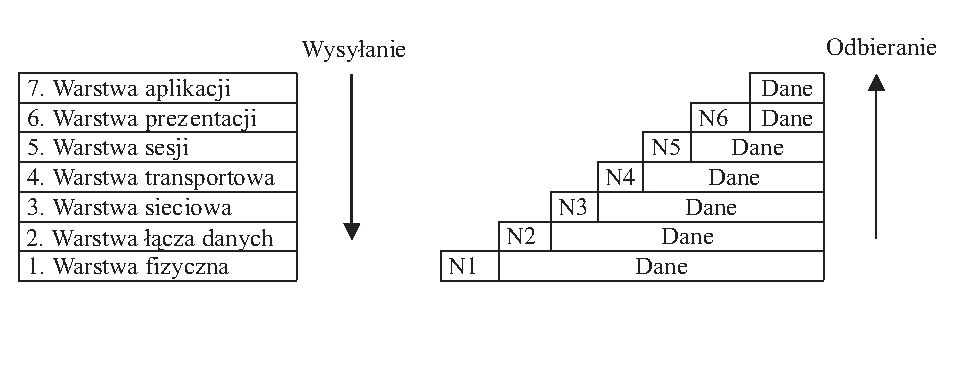
\includegraphics[width=5in]{./rysunki/nadawanie_i_odbieranie_naglowkow.eps}
\caption{Proces nadawania i odbierania nagłówków transmitowanym danym}
\label{nadawanie}
\end{figure}

Protokoły poszczególnych warstw zarządzają danymi w specyficzny dla siebie sposób, mogą np. dokonać segmentacji, 
czyli podziału danych na mniejsze fragmenty przed przesłaniem ich do niższej warstwy. Każdy fragment otrzymuje 
wtedy odpowiedni nagłówek, który umożliwia analogicznemu protokołowi w komputerze adresata danych scalenie 
fragmentów podczas odbierania pakietu. Nagłówki umożliwiają również zarządzanie połączeniami np. 
multipleksowanie połączeń czyli wykorzystywanie jednego połączenia, ściślej -- punktu dostarczania usług SAP 
(ang. \emph{Service Access Point})  warstwy niższej, np. sieciowej do obsługi kilku połączeń nawiązanych w warstwie 
bezpośrednio wyższej (tu transportowej). Odpowiednia informacja zawarta w nagłówku warstwy wyższej umożliwia 
wtedy identyfikację odbiorcy danych. Model ISO/OSI definiuje dwa tryby komunikacji. Komunikacje połączeniową 
stosuje się gdy kluczowym wymaganiem jest niezawodność transmisji, musi być wtedy znany zarówno odbiorca jak i 
nadawca danych, a odbiorca potwierdza dotarcie do niego każdego fragmentu pakietu lub sygnalizuje konieczność 
retransmisji w przypadku błędu. Komunikacja bezpołączeniowa nie zapewnia niezawodności, dane wysyła się bez 
oczekiwania na potwierdzenie, a nadawca  i odbiorca nie są znani, chyba że wynika to z zawartości pakietu, 
pakiety wysyłane w trybie bezpołączeniowym nazywamy datagramami.

W praktyce nie istnieje rozwiązanie przemysłowe, które ściśle implementowałoby wszystkie warstwy modelu ISO/OSI, 
częstą praktyką jest np. łączenie warstw fizycznej i łącza danych w jedną warstwę. Również protokoły TCP/IP nie 
są w pełni kompatybilne z modelem ISO/OSI, nie są też jednak całkowicie niekompatybilne. Wzajemną relację 
architektury ISO/OSI i TCP/IP przedstawia poniższy rysunek \cite{barylo1}.
\begin{figure}[h]
\centering
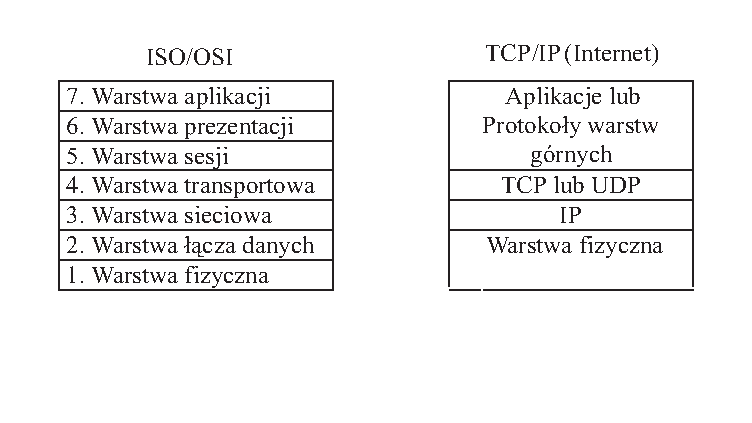
\includegraphics[width=5in]{./rysunki/architektura_ISO_a_tcp.eps}
\caption{Architektura ISO/OSI a TCP/IP}
\label{ISO_TCP}
\end{figure}
\section{Protokół IP}

Protokół IP (ang. \emph{Internet Protocol}) działa w warstwie sieciowej i jest podstawowym protokołem rodziny TCP/IP --
wszystkie dane napływające z wyższych warstw przesyłane są w sieci jako datagramy IP. Protokół ten świadczy 
zawodne, bezpołączeniowe usługi dostarczania pakietów. Przez zawodne rozumiemy tu taką właściwość, że IP nie 
daje gwarancji dostarczenia pakietu do punktu przeznaczenia, a wszelkie mechanizmy zapewnienia niezawodności transmisji muszą
zostać zapewnione przez protokoły wyższych warstw (np. TCP). Termin bezpołączeniowy oznacza tu, że IP nie 
przechowuje żadnej informacji na temat prawidłowo przesyłanych datagramów, każdy z nich obsługiwany jest osobno, 
co w praktyce może oznaczać, że datagramy mogą docierać do adresata w innej kolejności, niż zostały wysłane. 
Wszystkie dane konieczne do poprawnej pracy IP zawarte są w jego nagłówku, który typowo (jeśli nie zawiera 
opcji) ma długość 20 bajtów i przedstawiony poniżej format \cite{barylo2}.

\begin{figure}[h]
\centering
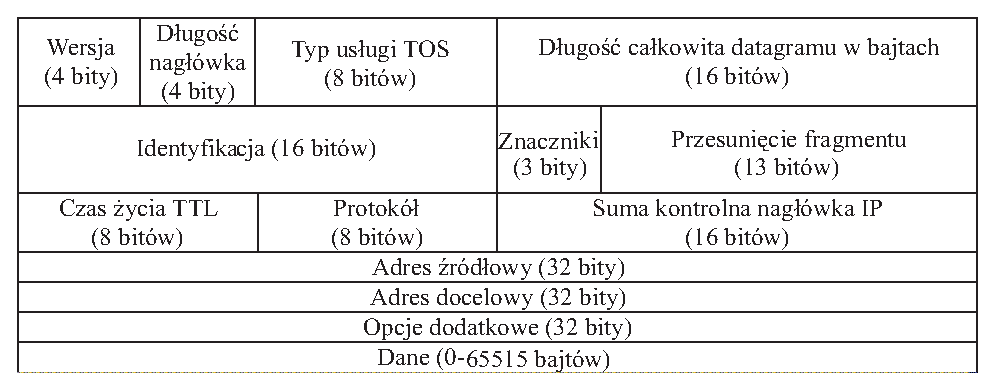
\includegraphics[width=5in]{./rysunki/datagram_ip.eps}
\caption{Format datagramu IP z wyróżnieniem nagłówka}
\label{datagram_ip}
\end{figure}

Pole \emph{długość nagłówka} określa długość nagłówka w 32--bitowych słowach i wraz z polem Długość całkowita datagramu 
służy do określenia miejsca w którym zaczynają się właściwe dane. Całkowita długość datagramu ograniczona jest 
zwykle przez warstwę fizyczną np. dla sieci Ethernet jest to maksymalnie 1500 bajtów a wielkość tę nazywamy MTU 
(ang. \emph{Maximum Transmission Unit}) danej sieci.

Pole \emph{identyfikacja} zawiera unikalny numer dla każdego wysyłanego datagramu. Jeżeli przechodząc przez kolejne 
węzły sieci datagram musi zostać podzielony, to wartość ta jest kopiowana do wszystkich nagłówków IP 
powstających fragmentów i wraz z wartością pola Przesunięcie fragmentu umożliwia poprawne scalenie datagramu w 
punkcie docelowym. Pomocne są w tym również wartości bitów pola Znaczniki. Ustawienie jednego z nich wskazuje, 
że istnieje kilka fragmentów datagramu, ustawienie drugiego zabrania fragmentacji datagramu.

Pole \emph{czas życia TTL} wyznacza  maksymalną liczbę routerów przez które może przejść datagram (routerem 
nazywamy tu specjalizowane urządzenie lub odpowiednio oprogramowany komputer służące do przekazywania datagramów 
pomiędzy sieciami różniącymi się w warstwie fizycznej np. Ethernet i Token Ring, lecz pracującymi w oparciu o 
wspólny protokół warstwy sieciowej - IP). Wartość tego pola jest wielkością całkowitą zmniejszaną o jeden przez 
każdy router, do którego dociera datagram. Datagram z wartością TTL równą 0 usuwany jest z sieci, co zapobiega 
krążeniu w niej błędnie zaadresowanych datagramów.

Pole \emph{protokół} określa typ protokołu będącego nadawcą datagramu i jednocześnie protokół który powinien 
odebrać datagram w punkcie docelowym.

Kluczowe znaczenie dla wyznaczania trasy przesyłania datagramu mają pola \emph{adres docelowy} i \emph{adres źródłowy}. Na 
podstawie wartości pola Adres docelowy protokół IP dynamicznie wyznacza kolejny węzeł sieci na drodze pakietu, 
proces ten nazywamy marszrutowaniem IP. Adres IP jest 32--bitowym numerem, który w sposób unikalny wyznacza 
miejsce podłączenia interfejsu sieciowego (karty sieciowej) do sieci. W adresie IP wyróżniamy część globalną 
określającą adres sieci i część lokalną identyfikującą komputer w konkretnej sieci. Istnieje pięć klas adresów IP (Rys.: \ref{klasy_ip}):
\begin{figure}[h]
\centering
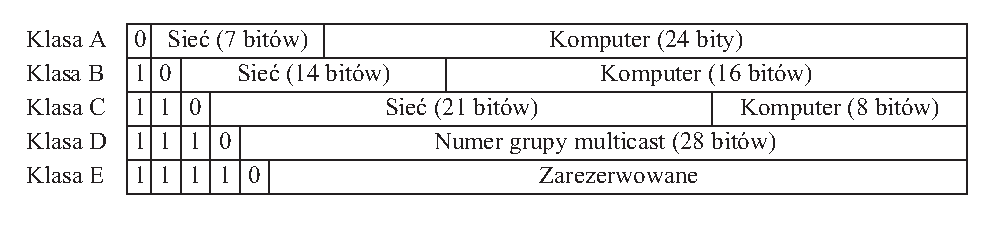
\includegraphics[width=5in]{./rysunki/klasy_adresow.eps}
\caption{Klasy adresów IP}
\label{klasy_ip}
\end{figure}

Aby zapewnić unikalność adresów sieci przydzielane są one centralnie przez organizację InterNIC. Adres zapisuje
się zwykle w tzw. notacji kropkowo -- dziesiętnej, dzieli się go na cztery ośmiobitowe  grupy i wartość każdej z 
nich zapisuje dziesiętnie np.156.17.130.10 jest adresem serwera pocztowego Instytutu Sterowania i Techniki Systemów
Politechniki Wrocławskiej.

Istnieją trzy typy adresów IP: adres unicast dotyczy pojedynczego komputera, adres broadcast dotyczy 
wszystkich komputerów w danej sieci a adres multicast obejmuje grupę komputerów należących do jednej grupy 
multicastowej. Obecnie wszystkie implementacje IP muszą obsługiwać tzw. adresowanie podsieci. Zamiast traktować 
adres IP jako proste złożenie adresu sieci i hosta (komputera) w części adresu wskazującej hosta wydziela się 
adres podsieci i właściwy adres hosta. Wynika to z faktu, że adresy klasy A i B przeznaczają zbyt wiele bitów na 
adres hosta, adres klasy B umożliwia np. zaadresowanie 65535 komputerów, a rzadko spotyka się tak wiele hostów 
podłączonych do jednej sieci. Podział 16 bitowego adresu hosta klasy B na dwie części ośmiobitowe umożliwia 
utworzenie w jednej sieci 255 podsieci z 254 hostami w każdej z nich. Decyzję o podziale na podsieci podejmuje 
lokalny administrator, a informację o tym jaka ilość bitów przeznaczona jest na adres podsieci przechowywana 
jest przez tzw. maskę podsieci. Jest to wartość 32--bitowa  zawierająca jedynki dla części adresującej sieć i 
podsieć oraz zera dla części adresującej hosta. Maska podsieci ma w omówionym przypadku postać 255.255.255.224.

Istnieje kilka zarezerwowanych adresów IP wykorzystywanych do celów specjalnych. Obowiązkowym adresem 
specjalnym jest adres interfejsu pętli zwrotnej (ang. \emph{loopback}). Większość systemów przypisuje temu interfejsowi 
z definicji adres 127.0.0.1, choć poprawny jest dowolny adres klasy A z adresem sieci 127. Datagramy kierowane 
na adres pętli zwrotnej przechodzą przez warstwę transportową i sieciową po czym są zawracane w górę stosu 
TCP/IP. Najczęstszym zastosowaniem pętli zwrotnej jest testowanie poprawności działania protokołów TCP/IP. 
Niektóre systemy (np. system AIX) umożliwiają dodawanie aliasów (dodatkowych adresów) do adresu interfejsu pętli 
zwrotnej.

Każdy komputer (host) podłączony do sieci IP posiada co najmniej jeden adres IP, hosty posiadające kilka 
interfejsów sieciowych posiadają po jednym adresie dla każdego interfejsu. Wszystkie te adresy, wraz z adresami 
specjalnymi i adresami typu broadcast przechowywane są w tzw. tablicy marszrutowania (routingu). Protokół IP po otrzymaniu 
datagramu sprawdza, czy jego adres IP zgodny jest z którymś z adresów hosta lub jednym z adresów specjalnych. 
Jeśli tak jest datagram zostaje zaakceptowany. Postępowanie w przeciwnym wypadku zależy od tego, czy warstwa IP 
skonfigurowana jest jako router. Jeżeli host nie jest routerem następuje odrzucenie datagramu, w przeciwnym wypadku
uruchamiany jest opisany poniżej algorytm marszrutowania.

Marszrutowanie IP dokonywane jest na podstawie kolejnych przejść pomiędzy węzłami sieci zapisanych (wraz z 
adresami własnymi hosta) w tablicy marszrutowania. Pojedynczy rekord tablicy routingu zawiera znany adres 
docelowy IP i adres IP na który należy skierować datagram jeśli jego adres docelowy jest zgodny z adresem 
zapisanym w rekordzie. Jeżeli nadawca i odbiorca są bezpośrednio połączeni rekord tablicy marszrutowania zawiera 
wskazanie (w postaci adresu IP) na adresata datagramu, o czym informuje specjalny znacznik w danym rekordzie. 
W przeciwnym wypadku jest to adres routera stanowiącego połączenie z inną siecią lokalną lub punkt wyjścia do 
sieci rozległej. Zakłada się że router taki znajduje się bliżej punktu docelowego datagramu, gdyż IP nie zna 
pełnej trasy dla żadnego z datagramów adresowanych poza sieć lokalną. Wybór drogi datagramu przebiega 
następująco \cite{barylo2}: 
w pierwszej kolejności poszukiwany jest rekord zawierający w pełni zgodny adres docelowy IP. Jeśli zostanie on 
znaleziony, datagram jest wysyłany na adres wskazany przez rekord. Może być to adres docelowy lub znane 
przejście przez router do innej sieci lokalnej.
Następnie w tablicy marszrutowania  poszukiwany jest rekord z adresem sieci zgodnym z adresem sieci 
marszroutowanego datagramu. Jeśli poszukiwania zakończą się sukcesem datagram jest wysyłany na zawarty tam adres. 
W ten sposób mogą być obsługiwane  datagramy zaadresowane do hostów połączonych z nadawcą przez wspólną sieć 
(w sensie zgodności adresów globalnych IP). 
W przypadku niepowodzenia poprzednich poszukiwań datagram wysyłany jest na adres IP routera domyślnego.

Ostatnią czynnością dokonywaną zanim datagram rzeczywiście opuści komputer nadawcy jest ustalenie jego adresu 
fizycznego w danej sieci lokalnej (np. adresu Ethernet lub Token Ring). Każde urządzenie: komputer, router, czy 
most (bridge) posiada unikalny w obszarze danej sieci lokalnej adres fizyczny. Odwzorowanie adresu IP w adres fizyczny 
dokonuje się przy użyciu protokołu ARP (ang. \emph{Address Resolution Protocol}), opis jego działania leży poza 
zakresem tej pracy.
Wypada zaznaczyć, że adresy IP klasy B wyczerpały się w roku 1997, co wymusiło wprowadzenie nowej specyfikacji
protokołu IP tzw. IPv6, który wprowadza adresy 128 bitowe. 

\section{Protokół TCP}

Protokół TCP (ang. \emph{Transmission Control Protocol}) zapewnia niezawodne, zorientowane 
połączeniowo, oparte na strumieniach bajtów (tzn. nie stosujące żadnego arbitralnego podziału przesyłanych 
danych na jednostki stałej długości) usługi warstwy transportowej. Przed rozpoczęciem transmisji dwie aplikacje 
używające TCP muszą ustanowić połączenie w postaci wirtualnego kanału transmisyjnego. Niezawodność tego 
połączenia zapewniana jest przez działania takie jak: podział przesyłanych danych na segmenty o rozmiarze 
optymalnym ze względu na poprawność transmisji; utrzymywanie dla każdego segmentu osobnego zestawu zegarów 
wyznaczających m. in. maksymalny czas oczekiwania na potwierdzenie odbioru segmentu i wymuszającego retransmisję 
w przypadku przekroczenia tego czasu; używanie obowiązkowych sum kontrolnych; odrzucanie zdublowanych 
datagramów IP; zdolność rozpoznania kolejności datagramów IP (mogą one docierać w kolejności innej niż były 
wysyłane).

Informację kontrolną segmentu TCP zawiera przedstawiony poniżej nagłówek \cite{barylo2}.
\begin{figure}[h]
\centering
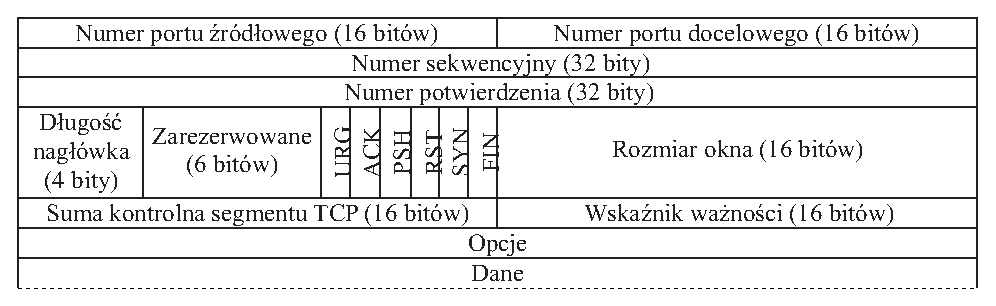
\includegraphics[width=5in]{./rysunki/format_segmentu_tcp.eps}
\caption{Format segmentu TCP z wyróżnieniem nagłówka.}
\label{segment_TCP}
\end{figure}

Pola \emph{numer portu źródłowego} i \emph{numer portu docelowego} zawierają wielkości całkowite i pełnią kluczową rolę w 
identyfikacji połączeń TCP. Numery portów od 1 do 1023 są zarezerwowane dla tzw. usług dobrze znanych i 
zazwyczaj przydzielane są aplikacjom pracującym jako serwery. Przykładowo serwery WWW (protokół HTTP) otrzymują 
numer portu 80, serwery FTP wykorzystują porty 20 i 21 a serwery pocztowe (SMTP) port 25. Do nawiązania 
połączenia proces klienta (np. przeglądarka WWW) uzyskuje od protokołu TCP tzw. numer krótkotrwały unikalny dla 
każdej aplikacji używającej TCP w danym hoście. W przypadku przeglądarki WWW może być to numer 80 lub dowolny 
numer z zakresu 1024... 5000. Para port źródłowy -- port docelowy jest wystarczająca do identyfikacji połączenia 
po stronie klienta. Jeśli nawet użytkownik uruchomi dwie identyczne aplikacje (np. dwie przeglądarki WWW), to 
otrzymają one różne numery krótkotrwałe. Po stronie serwera sytuacja jest trudniejsza, typowo serwer poprzez 
multipleksację portu obsługuje wiele połączeń z użyciem jednego numeru portu źródłowego (np. 80 dla serwera WWW),
może się więc zdarzyć, że dwóch niezależnych klientów zgłosi ten sam numer krótkotrwały portu docelowego. Do 
jednoznacznej identyfikacji połączeń wykorzystuje się kombinację numeru portu i adresu IP nazywaną gniazdem. 
Gniazda są jednym z podstawowych pojęć interfejsu programisty TCP/IP.

Jak już wspomniano TCP przesyła dane w postaci strumienia bajtów, w praktyce oznacza to, że wysyłany 
segment danych może mieć każdorazowo inną  długość. Do umożliwienia uformowania z segmentów oryginalnego pakietu 
służy wartość pola \emph{numer sekwencyjny}. Jeśli rozpatrzymy strumień bajtów przesyłany tylko w jedną stronę, to 
wartość tego pola określa  numer jaki ma w strumieniu ostatni bajt segmentu. Wartość początkową numeru 
sekwencyjnego ustala nadawca w momencie ustanawiania połączenia. Jeśli początkowym numerem sekwencyjnym było 
100, a pierwszy segment ma długość 1024 bajty, to jego numerem sekwencyjnym jest 1123. Pierwszy bajt kolejnego 
segmentu składającego się na pakiet będzie miał numer 1124, jeśli segment ten ma długość 125 bajtów, to jego 
numerem sekwencyjnym jest 1248. Koniec strumienia oznacza się przez ustawienie flagi bitowej FIN w nagłówku 
ostatniego segmentu.

TCP wymaga potwierdzeń odbioru każdego przesłanego segmentu. Służy do tego pole \emph{numer potwierdzenia}. Jeśli 
znów rozpatrywać przesyłanie danych w jedną tylko stronę, to po odebraniu segmentu o numerze sekwencyjnym 1123 
klient wysyła (pozbawiony danych) segment TCP z ustawioną flagą bitową ACK i wartością numeru potwierdzenia 1124 
(jest to numer kolejny oczekiwanego bajtu). Aby zapewnić niezależne przesyłanie danych w obydwu kierunkach, 
każda ze stron pamięta numery sekwencyjne wymienianych segmentów. Opisany powyżej segment potwierdzenia posiada 
więc ustalany przez jego nadawcę numer sekwencyjny (np. 136), który serwer musi potwierdzić ustawiając flagę ACK 
i umieszczając w polu Numer sekwencyjny odpowiednią wartość (tutaj 137). Konsekwencją takiej strategii wymiany 
potwierdzeń jest fakt, że w trakcie wymiany danych flaga ACK jest ciągle ustawiona (ma wartość logiczną 1).
Pole Długość nagłówka zawiera liczbę 32--bitowych słów składających się na nagłówek, następuje po nim 6 
zarezerwowanych bitów i kolejno 6 flag bitowych. Istotną flagą jest SYN, która jest ustawiona podczas wymiany 
segmentów nawiązujących połączenie i ustalania początkowych numerów sekwencyjnych. 

Pole \emph{rozmiar okna} zawiera wartość całkowitą, przy pomocy której odbiorca deklaruje jaką ilość bajtów 
nadawca może wysłać bez oczekiwania na potwierdzenie (inaczej -- jaką ilość bajtów odbiorca jest w stanie przyjąć 
jednorazowo). Pole ma zastosowanie w przypadku transmisji wg tzw. protokołu przesuwnego okna, a jego wartość 
może się zmieniać w trakcie  transmisji.

Ważną rolę w trakcie nawiązywania połączenia pełni pole \emph{opcje}. W polu tym uczestnicy połączenia wymieniają 
się informacją jak duży jest pojedynczy segment, który są w stanie przyjąć. Ustalone w ten sposób maksymalne 
wielkości segmentu MSS (ang. \emph{Maximum Segment Size}) pozostają stałe dla obydwu końcówek połączenia przez cały 
czas jego trwania. 

Wartość tę ustala się z uwzględnieniem nakładanego przez warstwę fizyczną ograniczenia na maksymalny rozmiar 
datagramu IP (MTU).

Aby móc zarządzać połączeniami oprogramowanie protokołu TCP utrzymuje tablicę połączeń. Pojedynczy rekord takiej 
tablicy opisuje jedno połączenie i zawiera pola: 
\begin{itemize}
\item Status (zamknięte, w trakcie zamykania, oczekiwanie na potwierdzenie itp.)
\item Adres lokalny -- adres IP hosta źródłowego (przechowującego tablicę)
\item Port lokalny -- numer portu hosta źródłowego
\item Adres zdalny -- adres IP hosta docelowego
\item Port zdalny -- numer portu docelowego
\end{itemize}

Protokół TCP wykorzystywany jest przez wiele protokołów wyższych warstw, dla których najistotniejszą sprawą jest 
zapewnienie niezawodności transmisji. TCP używają m. in. HTTP, FTP czy SMTP, które zostaną krótko omówione w 
dalszej części tej pracy. System DNS korzysta z protokołu TCP podczas wymiany danych pomiędzy serwerami DNS w 
trakcie uaktualniania ich tablic odwzorowań.

\section{Protokół UDP}

Protokół UDP (ang. \emph{User Datagram Protocol}) jest prostym, bezpołączeniowym protokołem warstwy transportowej 
wykorzystującym datagramy. Z każdego pakietu danych skierowanego do UDP przez warstwy górne formowany jest 
jeden datagram UDP, z którego (inaczej niż w przypadku TCP) tworzony jest dokładnie jeden datagram IP. Aplikacja 
wysyłająca pakiet musi sama zadbać o to, by jego długość nie przekroczyła MTU. UDP (w przeciwieństwie do TCP) 
nie implementuje żadnych mechanizmów zapewniających niezawodność transmisji.  Nagłówek datagramu UDP ma bardzo 
prosty format \cite{barylo2}.
\begin{figure}[h]
\centering
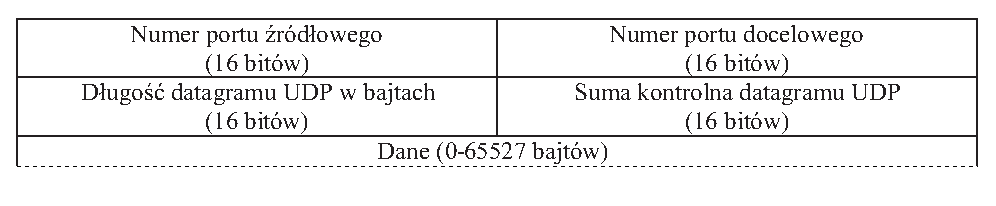
\includegraphics[width=5in]{./rysunki/datagram_udp.eps}
\caption{Datagram UDP z wyróżnionym nagłówkiem.}
\label{datagram_udp}
\end{figure}
 
\section{Protokół FTP}

Protokół FTP (ang. \emph{File Transfer Protocol}) jest standardowym w Internecie protokołem przesyłania dowolnego 
rodzaju plików. Jest to protokół warstw wyższych, i przez to jest często błędnie utożsamiany z aplikacjami 
klienta FTP. FTP korzysta w warstwie transportowej z usług protokołu TCP. Do obsługi transmisji FTP, w 
przeciwieństwie do większości protokołów, otwiera aż dwa połączenia TCP : połączenie sterujące o numerze portu 
docelowego 21 i połączenie transmisji danych o numerze portu 20. Przez połączenie sterujące aplikacje FTP 
wymieniają zdefiniowane w protokole polecenia i potwierdzenia. Połączenie transmisji używane jest do binarnego 
przesyłania danych. Schemat obsługi połączenia przez procesy klienta i serwera FTP przedstawia rysunek \ref{polaczenie_ftp}.
\begin{figure}[h]
\centering
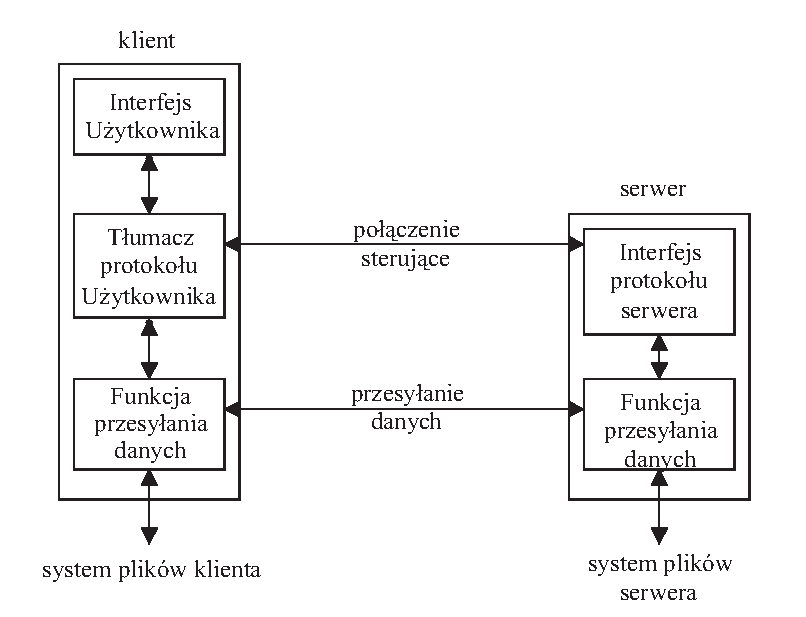
\includegraphics[width=5in]{./rysunki/obsluga_ftp.eps}
\caption{Obsługa połączenia ftp.}
\label{polaczenie_ftp}
\end{figure}

Połączenie przesyłania danych nawiązywane jest dla każdego przesyłanego pliku. FTP może przesyłać pliki w 
jednym z trzech trybów: jako strumień bajtów, jako serię bloków podzielonych nagłówkami lub w rzadko stosowanym 
trybie z kompresją FTP (kompresji podlegają tylko ciągi zerowych bajtów). FTP rozpoznaje formaty ASCII i EBCDIC 
-- przesyłane są one w postaci rekordów o stałej długości, pozostałe pliki traktowane są jako pliki binarne i 
przesyłane jako strumień bajtów.

Polecenia FTP wymieniane przez połączenie sterujące mają postać ciągów wielkich liter ASCII o długości 3 
lub 4 bajtów. Każde nawiązanie połączenia z serwerem FTP wymaga podania nazwy użytkownika i hasła, jest to 
prosty mechanizm zapewniający kontrolę dostępu do zasobów serwera. O tym, jakie pliki udostępniać konkretnym 
użytkownikom decyduje administrator serwera FTP.
Według badań prowadzonych w szkieletowej sieci NSFNET dane FTP stale stanowią ok. 20\% pakietów 
transmitowanych w tej sieci. 

\section{Protokół SNMP}

Protokół SNMP (ang. \emph{Simple Network Management Protocol}) pierwotnie zaprojektowano jako uniwersalne narzędzie, 
które umożliwi zdalne nadzorowanie śluz (ang. \emph{gateway})  i routerów w sieciach rozległych. W miarę jego rozwoju 
protokół uzupełniono o możliwość zarządzania wszelkim typem urządzeń sieciowych w sieciach TCP/IP. SNMP każdej 
sieci opiera się o trzy składniki:
\begin{itemize}
\item MIB (ang. \emph{Management Information Base}) jest to baza danych opisująca stan danego urządzenia;
\item SMI (ang. \emph{Structure and Identification of Management Information}) jest zestawem powszechnie stosowanych 
schematów służących odwoływaniu się do zmiennych MIB;
\item SNMP określa zasady komunikowania się pomiędzy aplikacją zarządzającą siecią (serwerem SNMP), a procesem 
sterującym urządzeniem (agentem).
\end{itemize}

Każdy element sieci, który ma być zarządzany przez SNMP, musi przechowywać informację o parametrach określających
stan danego elementu, a mających wpływ na pracę sieci. Baza danych zawierająca te parametry to właśnie MIB. W 
przypadku urządzenia takiego jak router rekord MIB może np. zawierać informację o stopniu zapełnienia jego 
buforów pamięci. MIB nie musi dotyczyć elementów ściśle sprzętowych istnieją np. MIB systemów operacyjnych. 
Sposób odwoływania się do elementów MIB określają schematy SMI.

W każdej sieci, której elementy zarządzane są według standardów SNMP istnieje wydzielony host, na którym 
pracuje specjalistyczna aplikacja (serwer SNMP) służąca monitorowaniu i zarządzaniu pracą sieci. Proces, który 
działa w zarządzanym elemencie i  aktualizuje MIB oraz udostępnia serwerowi jej zmienne lub ustawia je na zadane 
przez serwer wartości nazywany jest agentem SNMP.

W celu umożliwienia komunikacji pomiędzy serwerem a agentami SNMP definiuje pięć typów komunikatów. Trzy 
z nich wysyłane są zawsze w kierunku serwer--klient i służą pobieraniu lub ustawianiu zmiennych MIB. Dwa typy 
komunikatów wysyłane są w kierunku klient--serwer. Jeden z nich zwraca żądaną lub nowo ustawioną wartość 
zmiennej MIB, drugi jest komunikatem alarmowym wysyłanym przez agenta w przypadku błędnej pracy urządzenia lub 
przekroczenia krytycznej wartości przez którąś ze zmiennych MIB.
Serwer SNMP musi utrzymywać w miarę aktualną informację o stanie sieci, dlatego agenci SNMP przepytywani 
są w regularnych odstępach czasu, posiadając jednocześnie możliwość raportowania o sytuacjach awaryjnych. Fakt, 
że cztery z pięciu możliwych rodzajów komunikacji pomiędzy serwerem a agentem SNMP to pary typu pojedyncze 
pytanie--pojedyncza odpowiedź (wyjątek stanowią komunikaty alarmowe) oraz chęć minimalizacji obciążenia sieci 
powodowanego przez pakiety służące jej zarządzaniu spowodowały, że SNMP w warstwie transportowej korzysta z 
usług UDP. Zawodność tego protokołu sprawia, że serwery SNMP powinny (szczególnie w sytuacjach awaryjnych) 
stosować mechanizmy odmierzania czasu na odpowiedź agenta i ewentualnej retransmisji komunikatów. Warto dodać, 
że SNMP nie jest zależny w warstwie sieciowej od IP, przy odpowiedniej konfiguracji rolę protokołu sieciowego 
może spełniać np. IPX/SPX.

\section{Protokół SMTP}

Protokół SMTP (ang. \emph{Simple Mail Transfer Protocol}) jest prostym protokołem warstw górnych wykorzystywanym do 
przesyłania poczty elektronicznej w sieciach TCP/IP. W warstwie transportowej SMTP wykorzystuje protokół TCP i 
posiada przydzielony numer portu 25. Należy wyjaśnić, że programy pocztowe, z którymi kontaktują się szeregowi 
użytkownicy Internetu stanowią jedynie końcowe narzędzia, w terminologii fachowej nazywane agentami użytkownika 
UA (ang. \emph{User Agent}) służące do pobierania listów z elektronicznych skrzynek pocztowych lub umieszczania ich w 
kolejce do najbliższego serwera pocztowego. Programy rzeczywiście zajmujące się przesyłaniem wiadomości pomiędzy 
serwerami pocztowymi nazywane są agentami przesyłania komunikatów MTA (ang. \emph{Message Transfer Agent}). Przykładem 
MTA jest unixowy Sendmail. Protokół SMTP służy właśnie do komunikacji pomiędzy poszczególnymi MTA. Schemat 
przesyłania poczty w Internecie przedstawia poniższy rysunek.
\begin{figure}[h]
\centering
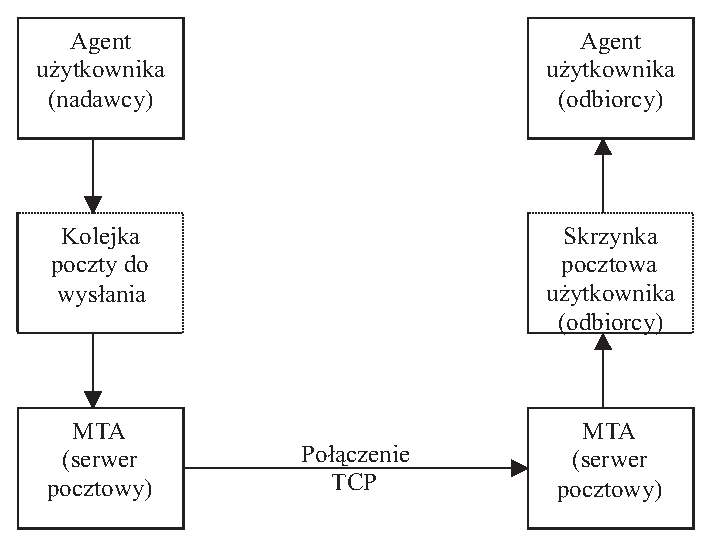
\includegraphics[width=5in]{./rysunki/obsluga_poczty.eps}
\caption{Schemat przesyłania poczty elektronicznej}
\label{poczta}
\end{figure}

Komunikacja pomiędzy MTA odbywa się według modelu klient -- serwer, przy czym klientem nazywamy MTA, który inicjuje dane 
połączenie. Połączenie rozpoczyna się od przesłania danych identyfikujących nadawcę, a w odpowiedzi nadchodzi pakiet 
identyfikujący odbiorcę. Następnie przesyłana jest właściwa wiadomość i połączenie jest zamykane. Do obsługi poczty 
elektronicznej SMTP definiuje tylko 13 poleceń (dla porównania FTP posiada 40 poleceń), które są czterobajtowymi ciągami 
wielkich liter ASCII.

Wiadomość elektroniczna składa się w SMTP z trzech części. Koperty czyli danych pozwalających MTA zidentyfikować 
nadawcę i odbiorcę wiadomości, nagłówków czyli danych wykorzystywanych przez agentów użytkownika (np. data 
wysłania wiadomości) i właściwej wiadomości.
Pakiety SMTP stanowią od 8 do 13 procent pakietów transmitowanych w sieci szkieletowej NSFNET. 

\section{Protokół POP3.}

Opisany powyżej protokół SMTP jest efektywnym narzędziem umożliwiającym przesyłanie poczty elektronicznej 
pomiędzy pracującymi w sposób ciągły serwerami SMTP. Aby pojedynczy użytkownik sieci mógł odbierać pocztę 
bezpośrednio przez SMTP w jego stacji roboczej musiałby ciągle działać proces typu MTA, co jest często 
niemożliwe ze względów czysto technicznych. Rozwiązanie tego problemu jest bardzo proste. W podłączonych do 
Internetu sieciach lokalnych wydziela się działający non--stop  serwer pocztowy wraz z oprogramowaniem 
zachowującym na dysku wiadomości nadchodzące do użytkowników sieci. Protokół POP3 (ang. \emph{Post Office Protocol 
version 3}) umożliwia dynamiczny dostęp do wiadomości przechowywanych na takim wydzielonym serwerze \cite{barylo9}. Protokół ten 
korzysta z TCP i numeru portu 110. POP3 definiuje 13 poleceń w postaci czterobajtowych ciągów ASCII. 

Połączenie POP3 rozpoczyna się od identyfikacji użytkownika i podania hasła następnie serwer i klient wymieniają 
dane po czym sesja kończy się.

Producenci aplikacji pocztowych (UA) stosują dwa protokoły, SMTP do bezpośredniego wysyłania poczty i POP3 
do odbierania jej z serwera pocztowego.

Pakiety POP3 najczęściej spotkać można w sieciach lokalnych, gdzie mogą stanowić znaczny procent 
transmitowanych danych.

\section{Protokół SSL}

Protokół SSL (ang. \emph{Secure Socket Layer}) jest protokołem rezydującym bezpośrednio nad protokołem TCP i 
dostarczającym dowolnemu protokołowi wyższych warstw (np. HTTP) przezroczyste usługi mające zapewnić poufność 
przesyłanych danych. SSL wykorzystuje port TCP o numerze 443. Bezpieczeństwo połączenia oparte jest o trzy cechy 
protokołu SSL: symetryczne szyfrowanie danych w oparciu o np. algorytmy DES lub RC4; autoryzację hostów z 
wykorzystaniem szyfrowania asymetrycznego lub z kluczem publicznym (RSA, DSS) i  kontrolę poprawności transmisji 
poprzez zastosowanie szyfrowanych sum kontrolnych MAC (ang. \emph{Message Autenthication Codes}).

W protokole SSL wyróżniamy dwie warstwy: warstwę powitania i warstwę rekordów. Warstwa powitania (ang. \emph{Handshake Layer}) 
inicjuje połączenie 
pomiędzy klientem a serwerem. Po wzajemnej identyfikacji hostów następuje faza negocjacji algorytmów, które będą 
użyte do szyfrowania transmisji (wybór ten zależy od mocy obliczeniowej hostów). Od momentu ustalenia sposobu 
kodowania wszystkie dane są szyfrowane.

Warstwa rekordów (ang. \emph{Record Layer}) rezyduje pomiędzy warstwą powitania a TCP i jest odpowiedzialna za 
enkapsulację danych napływających z wyższych warstw do postaci rekordów o maksymalnej długości 16384 bajtów, 
szyfrowanie rekordów oraz dołączanie MAC \cite{barylo10}.

Ponieważ SSL nie interpretuje napływających do niego danych istnieje możliwość przesyłania hipertekstu z 
użyciem SSL. Tak skonfigurowany serwer WWW nazywamy serwerem HTTPS lub serwerem SSL. Szyfrowane są wówczas 
wszystkie elementy  transmisji tzn. zarówno dokumenty jak i same polecenia HTTP, co wymaga odpowiedniej 
konfiguracji przeglądarki.

\section{URL i DNS}
	
Użytkownik Intrenetu do identyfikacji zasobów sieciowych stosuje zazwyczaj adres URL (ang. \emph{Uniform Resource 
Locator}). URL zapisujemy w postaci \cite{barylo5, barylo6}:\\
\emph{typ\_usługi://nazwa\_serwera.nazwa\_domeny/ścieżka\_dostępu/nazwa\_zasobu}. 
Na przykład URL http://www.netscape.com/main.html jest wskazaniem na zapisany w postaci pliku HTML 
dokument hipertekstowy main.html znajdujący się na ścieżce dostępu (może być to nazwa katalogu lub jej alias) 
News/Sport w serwerze home umieszczonym w domenie netscape.com. Dokument ten dostępny jest poprzez protokół 
HTTP.

Część URL określająca typ usługi interpretowana jest przez aplikację używaną do połączenia z Internetem 
np. przeglądarkę WWW. Ścieżka dostępu i nazwa zasobu przesyłane są do serwera i interpretowane przez jego system 
plików. Nazwa serwera i nazwa domeny są tylko nazwami symbolicznymi i muszą być zamienione na adres IP zanim 
zostanie nawiązane połączenie z serwerem. Zamiana ta możliwa jest dzięki systemowi DNS.

DNS (ang. \emph{Domain Name System}) jest rozproszoną bazą danych umieszczoną na wielu Internetowych hostach, 
które nazywamy serwerami DNS. Każdy komputer, który chce korzystać z DNS musi pamiętać w swojej konfiguracji 
adres IP najbliższego serwera DNS. Nazwa DNS może mieć długość do 63 znaków. Przestrzeń nazw DNS ma strukturę 
hierarchicznego, podzielonego na poziomy drzewa. Mówimy, że domena wyższego poziomu com zawiera domenę niższego 
poziomu netscape. Rysunek \ref{dns} przedstawia hierarchiczną organizację DNS \cite{barylo3}.
\begin{figure}[h]
\centering
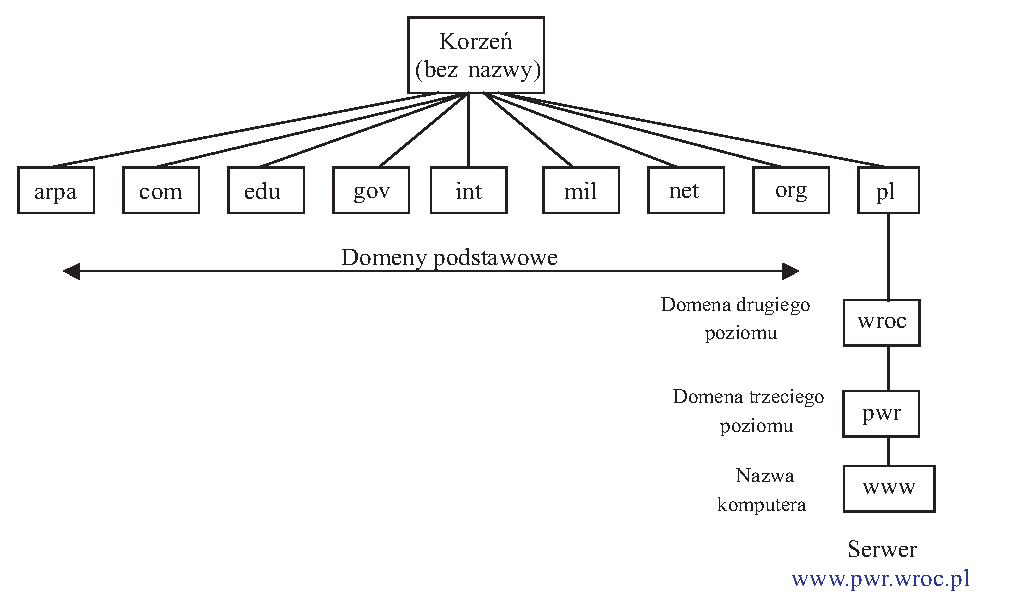
\includegraphics[width=5in]{./rysunki/struktura_dns.eps}
\caption{Hierarchiczna struktura DNS}
\label{dns}
\end{figure}
																
Domeny arpa, com, edu, gov, int, mil, net, org i domeny państwowe takie jak pl nazywamy domenami podstawowymi. 
Obejmują one następujące komputery: arpa -- sieć ARPANET; com -- organizacje komercyjne; edu -- instytucje edukacyjne; 
gov -- organizacje rządowe; int -- organizacje międzynarodowe; mil -- armia USA; net -- sieci; org -- pozostałe 
organizacje. Organizacje rządowe z krajów innych niż USA grupowane miały być w dwuliterowych domenach państwowych
np. ae -- Zjednoczone Emiraty Arabskie; pl -- Polska; zw -- Zimbabwe. Obecnie podział ten nie jest ściśle 
przestrzegany, wiele organizacji komercyjnych rejestruje się w domenie podstawowej (np. empik.com), inne stosują 
podział w ramach domen państwowych (np. creamsoft.com.pl). spotyka się również nazwy w ogóle nie mieszczące się 
w opisanym schemacie np. www.rmf.fm.

Obszarem nazywamy oddzielnie administrowaną część drzewa DNS. Typowym obszarem jest domena drugiego lub 
trzeciego poziomu  np. netscape.com lub pwr.wroc.pl. Jeśli w domenie zarejestrowanych jest wiele komputerów 
zwykle (dla zwiększenia efektywności działania DNS) dzieli się ją na kilka obszarów.

W każdym obszarze musi znajdować się podstawowy serwer DNS, który w specjalnym zestawie plików przechowuje 
odwzorowania wszystkich nazw komputerów z danego obszaru w ich adresy IP. Drugoplanowe serwery DNS informacje o 
odwzorowaniach uzyskują z serwera podstawowego korzystając z połączenia TCP o numerze portu 53. Serwery 
drugoplanowe przechowują (na zasadzie pamięci cache dla klientów, którzy zwracają się do nich z zapytaniami) 
odwzorowania obejmujące tylko część obszaru i odwzorowania o które klienci najczęściej pytają. W stałych 
odstępach czasu (typowo co 3 godziny) serwery drugoplanowe DNS uaktualniają swe tablice odpytując serwer 
podstawowy. Odwzorowanie nazwy spoza obszaru nie musi być znane ani serwerowi podstawowemu, ani drugoplanowemu, 
chyba że przechowywane jest w pamięci cache (jest często poszukiwane). Jeśli serwer podstawowy nie zna żądanego 
odwzorowania musi się zwrócić z zapytaniem (z wykorzystaniem portu 53 TCP) do jednego z serwerów głównych DNS 
(w 1993 roku było ich w Internecie 8), których obowiązkiem jest wskazanie serwera DNS będącego w stanie zwrócić 
poprawne odwzorowanie.

Proces odpowiedzialny za odwzorowanie nazw po stronie klienta nazywamy rezolwerem lub przelicznikiem nazw. 
Zwykle jest on zintegrowany z aplikacją (np. przeglądarką WWW) i na zasadzie pamięci cache przechowuje lokalnie 
pewną ilość odwzorowań. Jeśli wywoływana przez użytkownika nazwa nie jest znana lokalnie rezolwer korzystając z 
portu UDP 53 wysyła zapytanie do najbliższego drugoplanowego serwera DNS. Jeśli odpowiedź nie przekracza 512 
bajtów zwracana jest w postaci datagramu UDP, w przeciwnym wypadku jako datagram UDP wysyłane jest pierwsze 512 
bajtów i w nagłówku DNS ustawiana jest flaga informująca o tym fakcie. Zazwyczaj rezolwer ponawia wtedy 
zapytanie korzystając z portu 53 TCP, co umożliwia przesłanie pełnej odpowiedzi w jednym segmencie TCP. Rezolwer 
może wysłać dwa typy zapytań: zapytanie rekurencyjne umożliwia serwerowi DNS ,,konsultacje'' z serwerami wyższego 
rzędu przed zwróceniem odpowiedzi; zapytanie iteracyjne wymaga od niego natychmiastowej odpowiedzi, która jeśli 
dany serwer nie zna odwzorowania, musi mieć postać adresu IP serwera DNS będącego (wedle ,,wiedzy'' zapytanego 
serwera DNS) w stanie udzielić poprawnej odpowiedzi. Ze wskazanym serwerem DNS resolwer komunikuje się 
bezpośrednio. Ponieważ istnieje możliwość, że  nieprawidłowe zapytanie rekurencyjne nieskończenie będzie krążyć 
pomiędzy serwerami DNS w nagłówku DNS zdefiniowano pole ograniczające liczbę rekurencji. Wartość tego pola 
zmniejszana jest o jeden przez każdy serwer DNS, który przetwarza zapytanie. Zapytanie z zerową wartością tego 
pola jest odrzucane i serwer komunikuje błąd. W takim wypadku rezolwer może użyć zapytania iteracyjnego, ponowić 
zapytanie rekurencyjne ze zwiększoną wartością pola ograniczającego rekurencje lub zgłosić użytkownikowi błąd 
DNS. Rysunki \ref{rekurencyjne} i \ref{iteracyjne} przedstawiają obsługę obydwu typów zapytań \cite{barylo3}.
\begin{figure}[h]
\centering
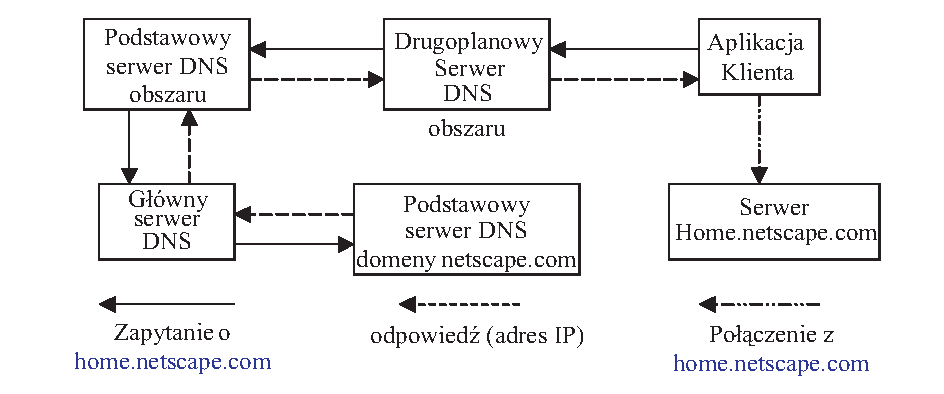
\includegraphics[width=4in]{./rysunki/zapytanie_rekurencyjne.eps}
\caption{Obsługa zapytania rekurencyjnego}
\label{rekurencyjne}
\end{figure}

\begin{figure}[h]
\centering
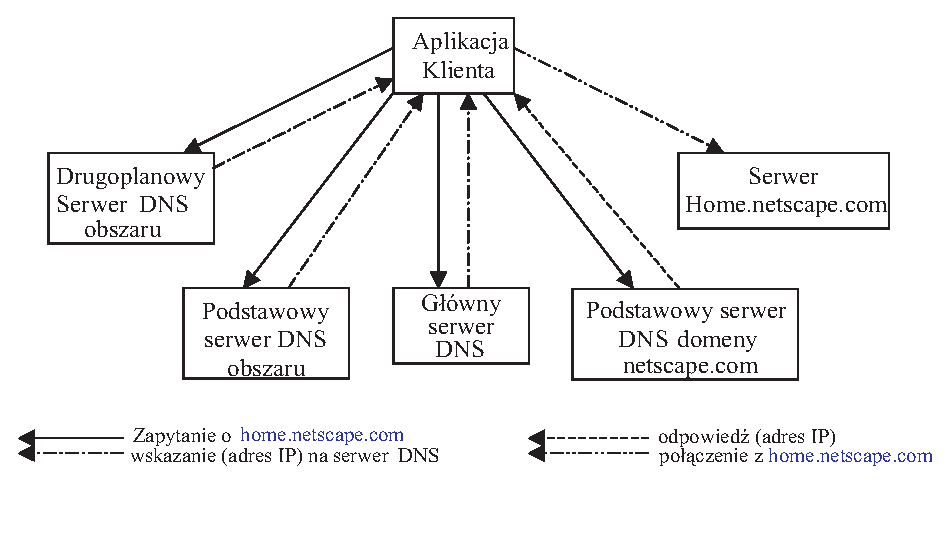
\includegraphics[width=4in]{./rysunki/zapytanie_iteracyjne.eps}
\caption{Obsługa zapytania iteracyjnego}
\label{iteracyjne}
\end{figure}

Powyższe rysunki przedstawiają ,,najgorszy'' przypadek, gdy adres IP serwera www.netscape.com znany jest dopiero 
przez podstawowy serwer DNS domeny (obszaru) netscape.com. W rzeczywistości istnieje duże prawdopodobieństwo, że 
odwzorowanie nazwy przechowywane jest przez pamięć cache jednego z bliższych klientowi serwerów.
Informacje o wzajemnych odwzorowaniach nazw w adresy IP serwery DNS przechowują w postaci rekordów zasobów 
DNS--DNS RR (ang. \emph{DNS Resource Record}). Rekordy te przesyłane są do aplikacji klienta jako odpowiedź na 
zapytanie. Pojedynczy DNS RR ma przedstawioną na rys. \ref{dns_rr} strukturę \cite{barylo3}.
\begin{figure}[h]
\centering
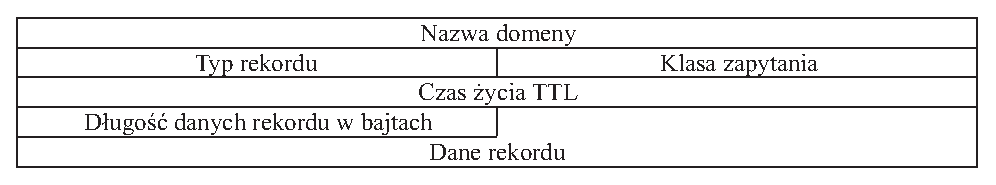
\includegraphics[width=5in]{./rysunki/format_dns_rr.eps}
\caption{Format DNS RR}
\label{dns_rr}
\end{figure}

Pole Nazwa domeny określa domenę do której odnoszą się dane rekordu. Pole Typ określa rodzaj danych np. czy 
rekord przechowuje odwzorowanie nazwy w adres IP, adresu w nazwę, czy tylko dodatkowe informacje o hoście. Pole 
Klasa ma zwykle wartość 1, co oznacza internetowy adres IP (niektóre serwery DNS udostępniają również adresy 
należące do innych protokołów np. IPX/SPX). Pole Czas życia TTL jest liczbą sekund określającą maksymalny czas 
przechowywania rekordu w pamięci cache rezolwera, niestety wiele aplikacji ignoruje tę wartość.

\section{Protokół HTTP}

W tym rozdziale 
szczegółowo omówiona jest specyfikacja protokołu HTTP oraz te właściwości protokołu, które rzutują na wydajność WWW.

\subsection{Specyfikacja HTTP}
 
Protokół HTTP (ang. \emph{HyperText Transfer Protocol}) jest prostym protokołem warstw górnych służącym do przesyłania 
dokumentów hipertekstowych w sieciach opartych o protokoły TCP/IP. W warstwie sieciowej HTTP korzysta z TCP i 
portu o numerze 80 \cite{barylo4}. 

Jak wspomniano dokument hipertekstowy zawierać może obok tekstu również grafikę, animacje, dźwięki oraz 
odsyłacze do innych dokumentów hipertekstowych, które mogą znajdować się na innych serwerach WWW, w konsekwencji 
często aby skompletować cały dokument przeglądarka WWW musi otworzyć wiele połączeń z kilkoma serwerami WWW.

HTTP wykonuje tylko przesyłanie plików składających się na dokument hipertekstowy. Jest to zazwyczaj plik 
będący opisem dokumentu w języku HTML, który zawiera tekst, informację o rozmieszczeniu elementów dokumentu oraz 
pliki będące reprezentacją takich elementów dokumentu jak grafika czy dźwięk. Ponieważ HTTP nie rozróżnia typów 
transmitowanych plików aplikacja serwera WWW jest dość prosta w porównaniu do aplikacji przeglądarki, która musi 
zinterpretować treść pliku HTML i odpowiednio rozmieścić na ekranie elementy dokumentu.

Istnieją dwa rodzaje komunikatów wymienianych pomiędzy klientem a serwerem HTTP: żądania i odpowiedzi. 
Format żądania HTTP ma następujący format:\\
	
	Linia--żądanie\\
	Nagłówki (0 lub więcej)\\
	<Linia pusta>\\
	Korpus (tylko dla żądania POST) \\

Format linii--żądania jest natomiast taki:\\
	
Dostępne są trzy różne żądania HTTP:
\begin{itemize}
\item żądanie GET, które zwraca dowolną informację (dokument) określoną przez następujący po nim URL;
\item żądanie HEAD, które zwraca tylko nagłówek wskazanego dokumentu, ten typ żądania wykorzystywany jest do sprawdzania 
odsyłaczy pod kątem aktualności lub dostępności;
\item żądanie POST używane do przesyłania danych od klienta do serwera np. przesyłania zawartości formularzy wypełnianych 
interakcyjnie przez użytkownika. Jest to jedyne żądanie wraz z którym przesyłany jest korpus komunikatu.
\end{itemize}

Format odpowiedzi HTTP jest następujący:\\

	Linia--stanu\\
	Nagłówki (0 lub więcej)\\
	<Linia pusta>\\
	Korpus\\

Format linii--stanu (status--line) ma następujący format:\\

	Wersja--HTTP kod--odpowiedzi fraza--odpowiedzi.\\

HTTP definiuje 17 różnych nagłówków, które dzielimy na 3 rodzaje: nagłówki używane z żądaniami, nagłówki używane 
z odpowiedziami, nagłówki określające korpus (przesyłane dane). Niektóre nagłówki mogą być używane zarówno z 
żądaniami jak i odpowiedziami (np. nagłówek DATE). Przykładowym nagłówkiem występującym z żądaniem jest nagłówek 
IF-MODIFIED-SINCE, który wraz z następującym po nim nagłówkiem DATE stanowi element tzw. warunkowego żądania 
GET. URL występujący w takim żądaniu jest otwierany tylko w przypadku jeśli był zmodyfikowany po wymienionej w 
żądaniu dacie. Jednym z nagłówków używanym z odpowiedziami jest LOCATION. Jego korpus stanowi nowy URL 
dokumentu, którego dotyczyło poprzednie zapytanie. Przykładem nagłówka określającego korpus jest LAST-MODIFIED. 
Następuje po nim nagłówek DATE, który podaje datę ostatniej modyfikacji dokumentu.
\begin{figure}[h]
\centering
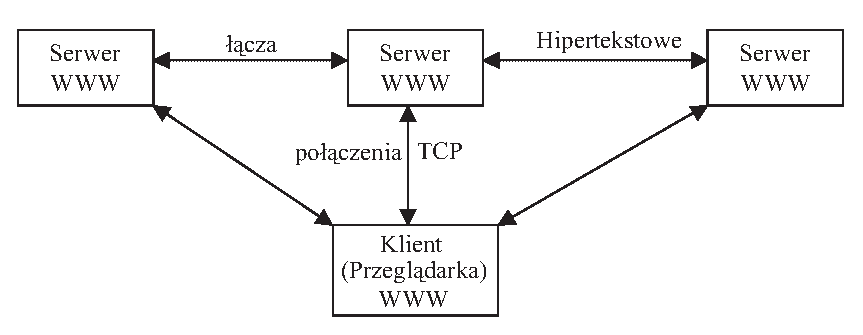
\includegraphics[width=5in]{./rysunki/polaczenia_w_sieci_www.eps}
\caption{Schemat połączeń w sieci WWW}
\label{polaczenia_www}
\end{figure}

Pierwsza linia odpowiedzi serwera nazywana jest linią stanu. Rozpoczyna ją określenie wersji HTTP, następnie 
podana jest trzycyfrowa liczba określająca kod odpowiedzi, a na końcu czytelne dla użytkownika wyrażenie. 
Poniższa tabela przedstawia znaczenie poszczególnych kodów odpowiedzi.

Starsze specyfikacje protokołu (HTTP 0.9 i HTTP 1.0) używały osobnego połączenia TCP do pobrania każdego 
elementu (pliku) wchodzącego w skład dokumentu. Najnowsza wersja HTTP 1.1 umożliwia stosowanie stałego, 
podzielonego na sesje połączenia TCP do pobrania całego dokumentu.

Poniżej omówiono istotne ze względu na wydajność WWW cechy protokołu HTTP.

\subsection{Właściwości ruchu generowanego przez HTTP, a wydajność WWW}

W okresie od stycznia 1994 do kwietnia 1995 udział komunikatów HTTP wśród wszystkich pakietów przesyłanych 
w szkieletowej sieci NSFNET wzrósł z 3\% do 36\% i wartość ta wykazywała stałą tendencję wzrostową. 

Badania prowadzone w USA wykazały niezależną od stopnia obciążenia serwera proporcję pomiędzy 
poszczególnymi typami żądań klienta. Żądania typu GET stanowią ok. 99\% ogółu komunikatów przetwarzanych przez 
serwer. 0,85\% komunikatów to żądania typu HEAD. Pozostałe 0,15\% stanowią żądania POST. 

Jeśli chodzi o odpowiedzi to 78\% do 92\% stanowią odpowiedzi typu 20x (odpowiedzi typu ,,sukces''). Odpowiedź typu 
304 obejmują 4\% do 14\% wysyłanych przez serwer komunikatów. Łącznie odpowiedzi typu 20x i 304 stanowią 92\% do 
97\% ogółu odpowiedzi. W przypadku pozostałych typów odpowiedzi różnice są już znaczne w zależności od rodzaju 
informacji na serwerze i jego popularności. Np. odpowiedzi 301 i 302 mogą mieć 0,3\% udział w odpowiedziach 
popularnego serwera publikującego informacje naukowe NCSA (ang. \emph{National Center for Supercomputer Applications}) 
do nawet 4,2\% w przypadku niewielkiego serwera uniwersyteckiego w Calgary. Odpowiedzi typu 40x i 50x stanowią 
zwykle od 1\% do 4\%. 

Typowo ilość danych przesyłanych w połączeniu HTTP jest niewielka. Żądania klienta nie przekraczają kilkuset 
bajtów, a pojedyncza odpowiedź serwera rzadko kiedy przekracza 10 kB.

Ciekawych informacji dostarczyć może analiza pomiaru czasu RTT (ang. \emph{Round Trip Time}), czyli łącznego czasu 
wymiany pakietu na drodze serwer -- klient -- serwer. Wartość ta jest używana przez TCP do wyznaczenia czasu 
retransmisji segmentu w przypadku braku potwierdzenia odbioru. Przybliżenie tego czasu można uzyskać dokonując 
pomiaru czasu trwania fazy zamykania połączenia TCP. Przytoczone tu wyniki otrzymano mierząc ten czas dla 19 
tyś. połączeń wykonanych przez 810 różnych klientów na terenie USA. Najmniejsza wartość wyniosła 0 sekund dla 
hosta lokalnego a największa 12,3 sekundy. Wartość średnia była równa 0,445 sekundy a mediana 0,187 sekundy. 
Wyniki te są zadziwiające jeśli wziąć pod uwagę, że teoretyczny RTT pomiędzy wschodnim i zachodnim wybrzeżem USA 
wynosi 0,06 sekundy. Odpowiedzialność za ten fakt ponosić może znaczna ilość klientów podłączonych poprzez modem 
(najszybszy nawet modem wprowadza ok. 0.2 sekundy opóźnienia do każdego pojedynczego pomiaru wartości RTT). 

Cechą bardzo niekorzystnie wpływającą na wydajność HTTP w jego starszych wersjach była konieczność otwierania 
osobnego połączenia TCP dla każdego elementu dokumentu. Wiele zależało tutaj od konstrukcji przeglądarki. Jeśli 
nie otwierała ona połączeń równoczesnych to pobranie całego dokumentu wydłużało się o czas konieczny na kolejne 
nawiązywanie i zamykanie połączeń. Jeśli z drugiej strony przeglądarka ,,agresywnie'' otwierała zbyt wiele 
połączeń równoczesnych, to barierą stawała się przepustowość połączenia z Internetem i wielkość MSS oferowana 
przez serwer. Znany jest przykład przeglądarki NCSA Mosaic, która potrafiła otworzyć kilkanaście równoczesnych 
połączeń TCP dla pobrania pojedynczego dokumentu, powodując tym zarówno zatory w sieci lokalnej jak i 
niepotrzebne obciążenie serwera. 

Otwieranie zbyt wielu połączeń równoczesnych nie przynosi spodziewanych korzyści. Podstawowym 
problemem wydajności HTTP wydaje się być niedopasowanie protokołu TCP -- zorientowanego na przesyłanie strumienia 
bajtów i usługi WWW zorientowanej na przesyłanie wyodrębnionych komunikatów. Należy pamiętać że HTTP, który jest 
w rzeczywistości protokołem przesyłania plików, miał w swych założeniach zapewniać wydajność większą niż 
protokół FTP. Chciano uzyskać to eliminując występujące w FTP dodatkowe połączenie sterujące (port 21) i 
konieczność nawiązywania połączenia TCP na dwóch portach. 

Niestety TCP wymaga zestawienia połączenia przed faktycznym rozpoczęciem transmisji. Wprowadza to opóźnienie o 
wartości ok. 1 RTT przed przesłaniem pliku. Dodatkowo w starszych wersjach HTTP pobranie dokumentu wymagało 
otwieranie nowego połączenia TCP dla każdego pliku składowego, co oznacza, że należało zamykać połączenia przez 
które wysłano wcześniejsze elementy dokumentu. Każdorazowe zamykanie i otwieranie połączeń wprowadza opóźnienie 
rzędu 3RTT dla każdego pliku składowego. HTTP 1.1 używa stałego łącza TCP dla dokumentu, co zredukowało 
opóźnienie przed rozpoczęciem transferu kolejnego elementu dokumentu do 1RTT. Dodatkowo HTTP 1.1 umożliwia 
wysyłanie żądań potokowych tzn. wysyłanie żądań o kolejne pliki przed rozpoczęciem odbierania poprzednio 
żądanych elementów dokumentu. Niestety w przypadku plików dynamicznych np. plików wynikowych skryptu CGI potok 
taki jest wstrzymywany. 
\chapter{Rozproszone serwery WWW}
\label{r03}
Rozdzia� ten przybli�y architektur� najcz�ciej wykorzystywan� w komunikacji tak pomi�dzy programami jak i
urz�dzeniami sieciowymi: architektur� klient--serwer. Nast�pnie zostanie przedstawiona budowa i dzia�anie serwera
WWW oraz wsp�pracuj�cego z nim klienta -- przegl�darki. Kolejnym punktem tego rozdzia�u b�dzie klasyfikacja
serwer�w WWW ze wzgl�du na wielko�� obs�ugiwanego ruchu jak i na charakterystyk� budowy i wymagania oraz
zwi�zane z tym definicje. W ostatnim punkcie tego rozdzia�u b�dzie przedstawiony spos�b testowania serwer�w webowych.

\section{Wprowadzenie}
Cz�sto�� i wydajno�� dostarczania us�ug WWW, przy stale zwi�kszaj�cej si� ich popularno�ci, 
stanowi nie lada problem dla tradycyjnych rozwi�za� klient--serwer. Zwi�kszenie dost�pno�ci
serwis�w mo�na osiagn�� modyfikuj�c poszczeg�lne elementy na drodze od klienta do serwera 
i/lub dodaj�c nowe. Na rys. \ref{www} przedstawiono cz�� element�w, kt�re wp�ywaj� na wydajno�� 
sieci Web.
\begin{figure}[h]
\centering
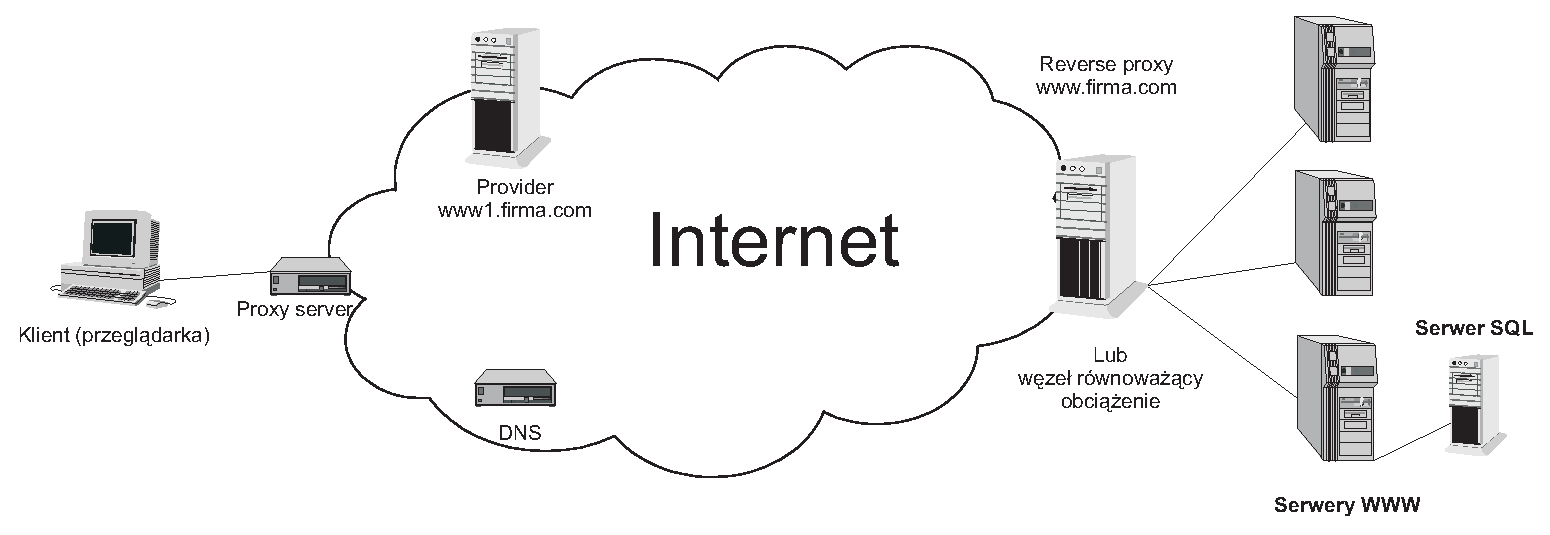
\includegraphics[width=\textwidth]{./rysunki/www.eps}
\caption{Przyk�adowe elementy stanowi�ce o wydajno�ci WWW}
\label{www}
\end{figure}

Najprostszymi s� \emph{cache} przegl�darki lub proxy serwer zainstalowany
po stronie klienta. Takie rozwi�zanie ma wiele zalet: prostota instalacji i konfiguracji, a przy
odpowiednich dokumentach (statyczny HTML) efektywno�� takiego rozwi�zania jest bardzo du�a. 
Wad� tych rozwi�za� jest g��wnie s�aba wydajno�� przy dokumentach generowanych dynamicznie
(a takich obecnie zdarza si� coraz wi�cej). Podobne rozwi�zanie mo�na zastosowa� po stronie 
serwera WWW, tzn. proxy, kt�re keszuje strony po stronie serwera(�w) -- nazywa si� ono 
\emph{reverse proxy}. 

Mo�na tak�e skorzysta� z us�ug r�nych dostawc�w (\emph{provider�w})
i przenie�� cz�� witryny WWW na ich komputery. Efektem b�dzie zwi�kszenie dost�pno�ci 
(oraz wydajno�ci) witryny, jednak�e za cen� mniejszego bezpiecze�stwa i zmniejszenia 
funkcjonalno�ci sajtu.

Mo�na zwi�ksza� wydajno�� w najprostszy spos�b --
poprzez dodawanie kolejnych procesor�w, pami�ci, dysk�w czy te� urz�dze� sieciowych. Jest to 
mo�liwe tylko w bardzo ograniczonym zakresie. 

Wydaje si�, �e najciekawszym rozwi�zaniem
jest wielokomputerowy serwer WWW. Zalet� wykorzystania wielokomputerowego serwera WWW
jest praktycznie nieograniczona skalowalno�� i wysoka dostepno��, wad� natomiast -- 
propagowanie ruchu na poszeg�lne jego sk�adowe (nody). Zarz�dzanie ruchem mo�na realizowa� na
szereg sposob�w: poprzez \emph{reverse proxy}, na poziomie serwera DNS, poprzez osobny w�ze�
r�wnowa��cy obci��enie, modyfikuj�c us�ugi po stronie klienta (opisane dalej applety Java), lub
serwera (metody te zosta�y opisane w rozdziale \ref{r03}). Wraz z architektur� takiego systemu zarz�dzaj�cego serwerem WWW
nale�y zaprojektowa� algorytmy umo�liwiaj�ce rozpraszanie ruchu sieciowego (Rozdzia� \ref{r04}).
Cz�� wy�ej wymienionych rozwi�za� mo�e by� tak iprogramowa jak i sprz�towa.

\section{Model klient--serwer}

\hspace{0.63cm}Model wsp�pracy klient--serwer to taki model, w kt�rym jeden program czeka pasywnie na ��danie komunikacji
wysy�ane przez inne programy. Okre�lenia klient i serwer odpowiadaj� dw�m programom zaanga�owanym w wymian� informacji.
Program inicjuj�cy po��czenie nazywany jest klientem, a program biernie czekaj�cy na ��danie po��czenia -- serwerem. Charakterystyka modelu \cite{siecikomputerowe}:

\begin{description}
\item[Oprogramowanie klienta]\
\begin{itemize}
\item dowolny program u�ytkowy, kt�ry staje si� klientem tymczasowo (w trakcie komunikacji), ale wykonuje r�wnie� obliczenia
lokalnie;
\item jest wywo�ywane bezpo�rednio przez u�ytkownika na czas obejmuj�cy jedn� sesj�;
\item dzia�a lokalnie na urz�dzeniu osobistym u�ytkownika;
\item aktywnie inicjuje po��czenie z serwerem;
\item w razie potrzeby mo�e komunikowa� si� z wieloma serwerami, jednak naraz aktywnie komunikuje si� tylko z jednym;
\item nie wymaga specjalnego sprz�tu, ani spesjalizowanego systemu operacyjnego.
\end{itemize}
\item[Oprogramowanie serwera]\
\begin{itemize}
\item jest specjalizowanym programem, kt�rego zadaniem jest �wiadczenie konkretnej us�ugi -- mo�e obs�ugiwa� naraz wielu
klient�w;
\item jest programem uruchamianym podczas startu systemu i dzia�a przez wiele kolejnych sesji;
\item dzia�a na publicznie dost�pnym komputerze;
\item czeka na zg�aszanie si� program�w klienckich;
\item pe�ni konkretn� us�ug�, ale po��czenia przyjmuje od dowolnych odleg�ych klient�w;
\item wymaga specjalnego sprz�tu i wyrafinowanego systemu operacyjnego.
\end{itemize}
\end{description}

\section{Architektura WWW}

\subsection{Serwer WWW}

\hspace{0.63cm}Najpro�ciej opisa� serwer WWW jako program wykonuj�cy w p�tli prost� operacj�: czekanie na otwarcie po��czenia przez klienta
(przegl�dark�) czyli na wysy�anie przez niego ��dania dost�pu do okre�lonej strony. W odpowiedzi serwer wysy�a ��dany dokument 
(lub komunikat o b��dzie w razie jego braku) albo przekazuje po��czenie do realizacji modu�owi (np. odpowiedzialnemu za obs�ug�
CGI) lub innemu serwerowi (np.: baz danych). nast�pnie serwer zamyka po��czenie i czeka na nast�pne. 

\subsection{Klient WWW -- przegl�darka}

\hspace{0.63cm}Przegl�darki WWW maj� bardziej z�o�on� budow� ni� serwery WWW. Obs�uguje ona wi�kszo�� zagadnie� zwi�zanych
z dost�pem do dokument�w i ich pokazywaniem u�ytkownikowi. W zwi�zku z tym sk�ada si� ona z szeregu du�ych modu��w, kt�re
ze sob� wsp�dzia�aj� \cite{siecikomputerowe}.

Koncepcyjnie przegl�darka sk�ada si� z zestawu klient�w, interpreter�w i modu�u, kt�ry tym wszystkim zarz�dza. Modu�
centralny -- zarz�dzaj�cy jest odpowiedzialny za interpretacj� danych z klawiatury i myszki oraz za wywo�ania pozosta�ych
modu��w w celu wykonania operacji ��danych przez u�ytkownika.

\begin{figure}[h]
\centering
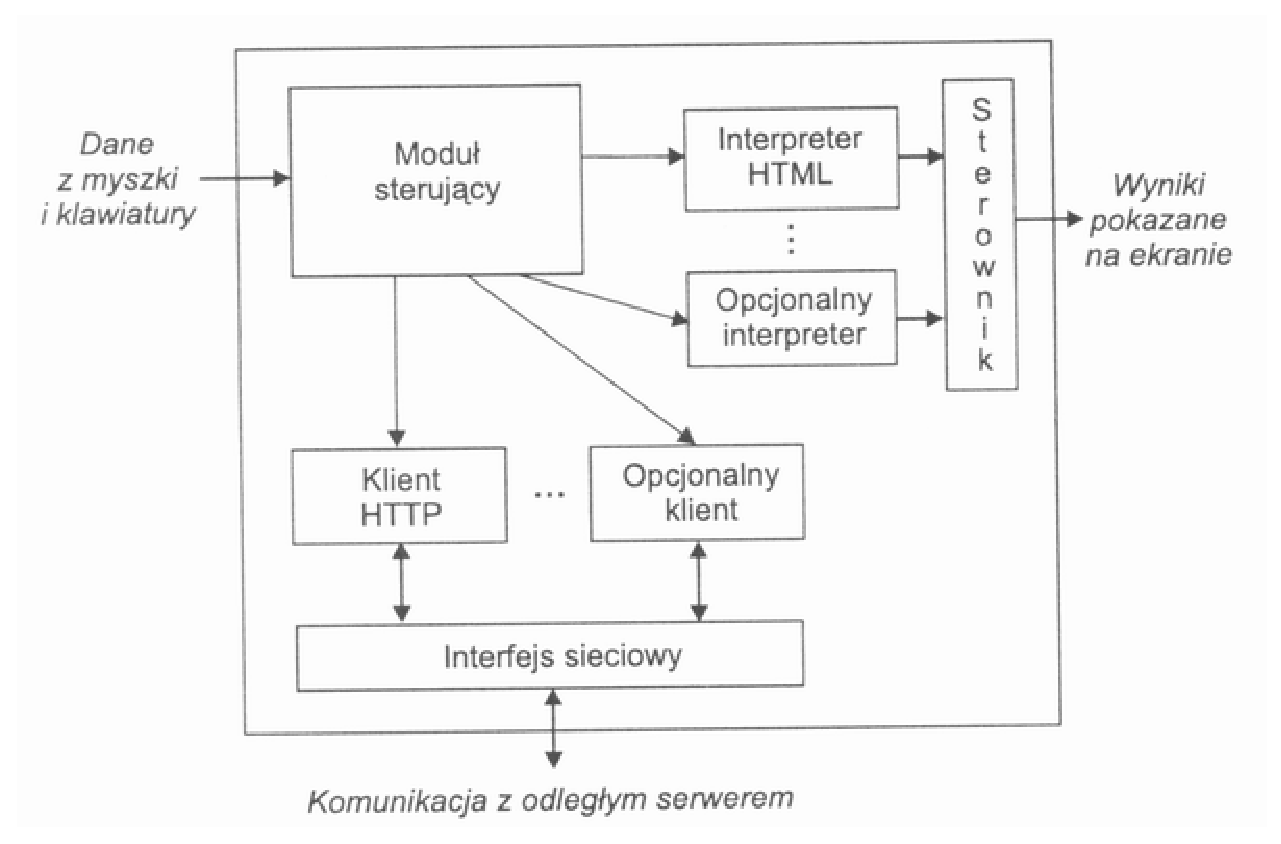
\includegraphics[width=4in]{./rysunki/przeg.eps}
\caption{G��wne sk�adniki przegl�darki WWW}
\label{przegl�darka}
\end{figure}

Ka�da przegl�darka musi zawiera� interpreter j�zyka HTML, �eby w og�le mog�a interpretowa� dokumenty WWW. Inne interpretery
s� opcjonalne, jednak�e powoli staj� si� r�wnie� niezb�dne -- takie jak interpreter Javy, czy XML. Dane dla interpretera
HTML stanowi dokument o zawarto�ci zgodnej ze sk�adni� tego j�zyka; wynikiem jego dzia�ania jest sformatowana posta�
dokumentu przez zamian� znacznik�w formatuj�cych na polecenia steruj�ce sprz�tem wy�wietlaj�cym informacje.

Jedn� z najwa�niejszych funkcji interpretera HTML jest obs�uga fragment�w dokumentu wybieralnych przez u�ytkownika.
Interpreter musi przechowywa� informacje o zwi�zku mi�dzy pozycjami na ekranie, a odsy�aczami w dokumencie HTML. Gdy
u�ytkownik wskazuje za pomoc� myszki pozycj� w dokumencie, interpreter HTML na podstawie bie��cej pozycji kursora i
zapami�tanych informacji ustala, kt�ry odsy�acz wskaza� u�ytkownik.

\subsection{Podzia� serwer�w WWW}

\hspace{0.63cm}Serwery WWW mo�na scharakteryzowa� g��wnie poprzez wielko�� (ilo�� realizacji ��da�) \cite{wybraneelementy}:
\begin{description}
\item[ma�e] -- uruchamiane na stacjach roboczych, zdolne do obs�u�enia do 5000 zapyta� dziennie, np.: prezentuj�ce dane jakiej�
niewielkiej firmy;
\item[�rednie] -- uruchamiane na du�ych serwerach posiadaj�cych zabezpieczenia na poziomie urz�dze� wewn�trznych. Obs�uguj�
kilkadziesi�t tysi�cy ��da� dziennie. Prezentuj� dane (tysi�ce stron) �redniej firmy;
\item[du�e] -- uruchamiane na serwerach o du�ej mocy obliczeniowej (zwykle kilku) posiadaj�cych techniki zabezpieczenia
danych i pracy serwer�w. S� w stanie obs�u�y� kilkaset tysi�cy zapyta� dziennie (prezentuj� kilkaset tysi�cy stron);
\item[globalne] -- s� w stanie obs�u�y� milion ��da� klienckich dziennie, prawie zawsze zbudowane z wielu du�ych serwer�w, 
posiadaj�ce kilka kopii dokumentu. S� wstanie udost�pnia� ogromne ilo�ci danych , r�wnie� multimedialnych.
\end{description}
W zale�no�ci od zawarto�ci witryn definiuje si� trzy klasy obci��alno�ci serwer�w WWW \cite{ScalableWebClusters}. Mamy zatem 
witryny typu:
\begin{description}
\item[web publishing] -- witryny zawieraj�ce statyczne i w niewiekiej ilo�ci dynamiczne dokumenty. Dokumenty statyczne s� 
sk�adowane na dyskach serwera webowego i nie podlegaj� modyfikacjom przez relatywnie d�ugi czas i zawsze s� przechowywane w 
pami�ci podr�cznej. Pami�� podr�czna ka�dego nodu klastra jest zwykle ustawiona na 15\% ca�kowitego drzewa dokument�w witryny.
Strony w niewielkim stopniu dynamiczne s� przechowywane w pami�ci podr�cznej (cache) z pradopodobie�stwem 0,3.
\item[web transaction (light)] -- s� to witryny zawieraj�ce oko�o 60\% dokument�w statycznych i oko�o 40\% stworzonych 
dynamicznie dokument�w. Zapytania bazodanowe do serwer�w \emph{back--endowych} wymagaj� intensywanego korzystania z dysk�w i 
st�d rezultaty zapyta� nie s� przechowywane w keszu.
\item[web transaction (heavy)] -- witryny zawieraj�ce 30\% statycznych dokument�w, 30\% niewiele zdynamizowanych dokument�w
oraz r�ne kombinacje (dla pozosta�ych 40\%) dokument�w, zwykle zawieraj�cych elementy wymagaj�ce sporych mocy obliczeniowych 
CPU i/lub dysku.
\end{description}

\section{Charakterystyka wydajno�ci serwera WWW}

Podstawow� miar� obci��enia serwera WWW jest ilo�� ��da� HTTP, kt�re docieraj� do niego w ci�gu sekundy. 
Za miar� wydajno�ci serwera mo�na przyj�� widziany od strony klienta czas odpowiedzi na ��danie lub czas 
uko�czenia transferu dokumentu, kt�ry zale�ny jest jednak od przepustowo�ci po��czenia klienta z Internetem. 
Przeprowadzone w USA symulacje z u�yciem prostego modelu serwera WWW, kt�ry oparto o teori� kolejek i za�o�enie, 
�e istotne s� tylko ��dania typu GET, s� podstaw� do przedstawienia poni�szych charakterystyk.
Typowo czas odpowiedzi na ��danie ro�nie wraz ze wzrostem liczby ��da� na sekund�. Wzrost ten jest 
pocz�tkowo bardzo powolny, niemal niezauwa�alny a� do momentu, w kt�rym ilo�� r�wnocze�nie otwartych po��cze� 
TCP przekracza mo�liwo�ci obs�ugi ich przez serwer. Przedstawia rysunek \ref{zapytania}[26].
\begin{figure}[h]
\centering
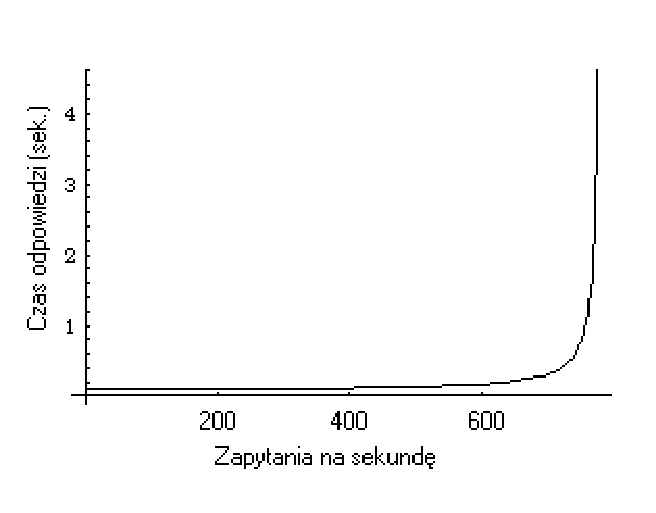
\includegraphics[width=3in]{./rysunki/zapytania.eps}
\caption{Czas odpowiedzi a ilo�� zapyta� na sekund�.}
\label{zapytania}
\end{figure}

Obci��enie przy kt�rym serwer za�amuje si� zale�y oczywi�cie od 
sprz�towych w�asno�ci serwera i zastosowanego oprogramowania. Opr�cz cech samego serwera najistotniejsze dla 
czasu odpowiedzi s� przepustowo�� po��czenia z Internetem oraz �redni rozmiar plik�w wysy�anych przez serwer. 
�redni rozmiar pliku zale�y w g��wnej mierze od rodzaju informacji publikowanych na serwerze (b�dzie on np. du�y 
na serwerze oferuj�cym wiele plik�w video). Po��dane jest jednak ,,oszcz�dne'' projektowanie stron WWW, gdy� 
wzrost �redniego rozmiaru pliku powoduje szybki spadek ilo�ci zapyta� na sekund� mo�liwych do obs�u�enia. 
Opisane zachowanie 
serwera powoduj�ce za�amanie si� jego wydajno�ci po przekroczeniu maksymalnej liczby zapyta� na sekund� jest 
typowe dla implementacji nie posiadaj�cych ograniczenia na maksymaln� liczb� jednoczesnych po��cze� TCP. Dotyczy 
to wi�kszo�ci system�w UNIX--owych, w kt�rych procesy serwer�w WWW wykonuj� standardow� akcj� fork--and--exec dla 
ka�dego nowego ��dania HTTP. Prostym rozwi�zaniem tego problemu wydaje si� wprowadzenie ograniczenia na liczb� 
po��cze� TCP. Wymaga�oby to jednak zmian w protokole HTTP (np. wprowadzenie odpowiedzi typu ,,serwer zaj�ty --
spr�buj p�niej'') oraz odpowiednich zmian w przegl�darkach.

Powy�sze rozwa�ania dotycz� wydajno�ci serwera widzianej od strony klienta. W przypadku laboratoryjnych 
bada� wydajno�ci �atwiej ni� czas odpowiedzi mo�na zmierzy� ilo�� zapyta� na sekund� obs�ugiwan� przez serwer. 
Jest to miara wydajno�ci bezpo�rednio koresponduj�ca z czasem odpowiedzi serwera (im wi�cej zapyta� serwer mo�e 
obs�u�y�, tym mniejszy jest jego czas reakcji) i wolna od wp�ywu takich czynnik�w jak wydajno�� przy��cza po 
stronie klienta.
Ci�g�y wzrost liczby u�ytkownik�w Internetu stawia coraz wi�ksze wymagania co do wydajno�ci serwer�w WWW. Do tego faktu dochodzi jeszcze jeden - charakterystyka ruchu WWW - opr�cz serwowania stron statycznych, dochodz� dynamiczne i obs�uga po��cze� szyfrowanych. 
W jaki spos�b zmienia si� wtedy wykorzystanie poszczeg�lnych element�w wida� na rys.\ref{charakterystyka}
\begin{figure}[h]
\centering
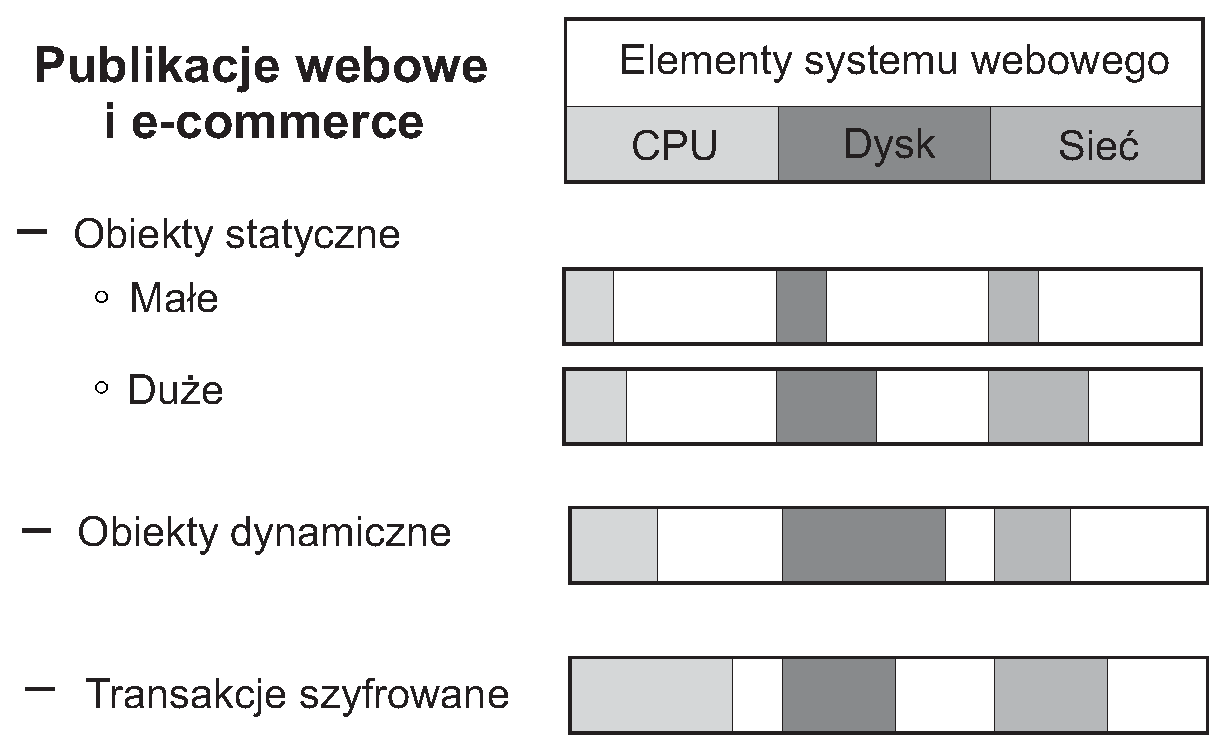
\includegraphics[width=3in]{./rysunki/charakterystyka_ruchu.eps}
\caption{Obci��enie poszczeg�lnych element�w serwera WWW w zale�no�ci od typu po��czenia.}
\label{charakterystyka}
\end{figure}

Pr�dzej czy p�niej ka�dy administrator takiego serwera stanie przed problemem znalezienia sposobu na 
zwi�kszenie jego wydajno�ci. Zwykle ze wzgl�du na specyfik� publikowanych informacji niewiele mo�na zrobi� ze 
�rednim rozmiarem przesy�anego pliku. Podstawow� metod� zwi�kszenia wydajno�ci serwera jest zwi�kszenie 
przepustowo�ci przy��cza. Sprz�towa modernizacja samego serwera nie przyniesie rezultat�w w przypadku gdy 
,,w�skim gard�emi'' jest przy��cze. Je�li jednak dysponujemy odpowiednio wydajnym przy��czem (np. lini� ATM) 
,,w�skim gard�em'' jest na pewno serwer. 

Wydajno�� ka�dego komputera zwi�kszy� mo�na dokupuj�c wi�ksz� ilo�� pami�ci RAM i szybsze dyski twarde. 
W przypadku serwer�w WWW jest to jednak rozwi�zanie prowizoryczne. Lepsze efekty przynosi instalacja maszyny 
wieloprocesorowej. Niestety obecne implementacje TCP/IP nie wykorzystuj� wielow�tkowo�ci w stopniu, kt�ry 
umo�liwia�by pe�ne wykorzystanie cech technologii wieloprocesorowej. Nale�y si� spodziewa�, �e otwartych 
po��cze� TCP b�dzie typowo wi�cej ni� procesor�w w serwerze. Gdyby obs�ug� stosu TCP/IP podzieli� mo�na by�o na 
niezale�ne w�tki, kt�rych wykonanie przebiega� by mog�o z podzia�em czasu, to efektywno�� wieloprocesorowych 
serwer�w WWW by�aby znacznie wi�ksza ni� obecnie. Wsp�cze�nie stosowanie serwer�w wieloprocesorowych nie 
przynosi korzy�ci tak du�ych jak spodziewane. 
Dobr� metod� zwi�kszenia wydajno�ci WWW jest stosowanie serwer�w proxy, kt�re na zasadzie pami�ci cache 
przechowuj� cz�� dokument�w serwisu i w ten spos�b cz�ciowo wyr�czaj� serwer g��wny. 
Najbardziej efektywn� i jednocze�nie najbardziej zaawansowan� technologicznie metod� zwi�kszenia 
wydajno�ci serwera WWW jest powielenie jego zawarto�ci na jeden lub kilka dodatkowych serwer�w i udost�pnienie 
tej grupy pod jednym adresem IP. Rozwi�zanie takie wymaga sprz�tu lub oprogramowania, kt�re z jednej strony 
ukrywa�oby przed u�ytkownikami istnienie kilku serwer�w o jednakowej zawarto�ci a z drugiej dokonywa�oby 
dystrybucji obci��enia pomi�dzy te serwery w spos�b maksymalizuj�cy ich ��czn� wydajno��.

\subsection{Serwery wielokomputerowe -- rozproszone}

\hspace{0.63cm}�eby serwery WWW by�y wydajne oraz mog�y pracowa� bez przerwy przez 365 dni w roku 24 godz. 
na dob� -- nie mog� pracowa� na jednym komputerze; wydajno��, skalowalno�� a przede wszystkim odporno�� na 
awarie mo�e zosta� zrealizowana jedynie poprzez rozproszone serwery WWW, w kt�rych zapytania od klient�w s�
w odpowiedni spos�b dystrybuowane do poszczeg�lnych serwer�w \cite{metodyalgorytmy}. 

�wiatowy trend w wykorzystywaniu na r�ne sposoby technologii World Wide Web jest coraz wi�kszy.
Znakomite darmowe serwery WWW (Apache, NCSA itp.), spora ilo�� przegl�darek internetowych
oraz olbrzymi rozw�j internetu \cite{siecikomputerowe}, a tak�e ogrone mo�liwo�ci tej us�ugi spowodowa�y zwi�kszone 
zainteresowanie t� technologi�.
Jednym z ostatnich nies�ychanie modnych technologii internetowych wykorzystuj�cych WWW jest handel 
elektroniczny skierowany tak do pojedynczego odbiorcy (\emph{Business to Customer-- B2C}) jak i wsp�pracuj�cych
firm (\emph{Business to Business}-- B2B). Poza tym r�wnie� bardzo interesuj�cym celem s� serwery aplikacyjne.
Powoduje to jednak�e konieczno�� utrzymania w sprawno�ci serwisu przez ca�y rok -- bez 
przerwy. Nie oznacza to wy��cznie mo�liwo�ci korzystania z tych serwer�w, czyli bezawaryjnej pracy, ale r�wnie�
uzyskanie jak najlepszego komfortu pracy z tymi systemami. Poza tym jeszcze jedn� nies�ychanie istotn� rzecz�
przemawiaj�c� za wielokomputerowymi serwerami WWW jest ich znakomita skalowalno�� (du�o ta�sza od skalowalno�ci
pojedynczych maszyn, kt�re nie zawsze dadz� si� rozbudowywa�). Takich zalet nie posiada pojedyncza maszyna. Jej koszt zakupu, 
a tak�e koszt rozbudowy -- przy zapewnieniu bezpiecze�stwa i odporno�ci na uszkodzenia jest olbrzymi. Fakt, �e pojedyncz�
maszyn� �atwiej si� administruje nie rekompensuje w pe�ni u�omno�ci architektury von Neumanna. Wielokomputerowe serwery
(nie tylko WWW, ale tak�e serwery obliczeniowe) mog� osi�ga� zawrotne wydajno�ci, s� praktycznie w niesko�czono�� skalowalne,
nadmiarowo�� tanich element�w (zamiast kupowa� trzy maszyny klasy mainframe -- mo�na kupi� sto komputer�w klasy PC) decyduje
o ich odporno�ci na uszkodzenia. Najlepszym przyk�adem jako�ci tej technologii jest najpot�niejsza z wyszukiwarek sieciowych --
GOOGLE\footnote{\emph{www.google.com}} pracuj�ca na kilku tysi�cach komputerow klasy PC, a zawieraj�ca w swojej bazie informacje 
o ponad miliardzie trzystu milionach stron WWW (jest wykorzystywana przez wi�kszo�� serwis�w webowych). Wad�
system�w klastrowych jest administracja i spos�b wsp�dzielenia obci��enia pomi�dzy poszczeg�lnymi nodami (istnieje jednak�e
oprogramowanie darmowe umo�liwiaj�ce r�wnowa�enie obci��enia serwer�w WWW\footnote{\emph{www.linuxvirtualserver.org}}, a 
tak�e serwer�w obliczeniowych\footnote{\emph{www.mosix.org}}).

Trend ten nie znajduje odzwierciedlenia tylko w serwerach webowych. Konstrukcja wielokomputerowa pozwala na znacznie 
efektywniejsze zarz�dzanie zasobami i przydzieleniem zada� do zasob�w. Pozwala tak�e uzyska� ,,prawdziwe'' zr�wnoleglenie
oblicze� -- brak jest tu ,,kombinowanych'' metod uwsp�lniania zasob�w i rozdzia�u ��da� do magistral i pami�ci obecnych
w typowych architekturach. Kolejn� zalet� system�w nieneumanowskich jest mo�liwo�� zapewnienia bezpiecze�stwa ci�g�o�ci
pracy w spos�b dot�d niewykonalny. Przyk�adem spe�nienia wszystkich tych cech s� wsp�czesne superkomputery i mainframy, 
z kt�rych do�wiadcze� korzystali wsp�cze�ni tw�rcy nowoczesnych, skalowalnych technik webowych. Ka�dy superkomputer (SGI,
Hitachi, NEC, Intel, IBM) oraz system mainframowy (g��wnie IBM) sk�ada si� z szeregu (nawet kilkudziesi�ciu) nod�w 
skonsolidowanych zwykle w jednej obudowie, a po��czonych wysokoprzepustow� sieci� transmisyjn�. St�d wiele pomys��w zosta�o
zaczerpni�tych i wykorzystanych przy tworzeniu rozposzonych architektur webowych.

Klasyczny system komputerowy obs�uguj�cy serwer webowy jest obs�ugiwany niskopoziomowo -- system operacyjny obs�uguj�cy
serwer webowy. W architekturze rozproszonego webu pomi�dzy systemem operacyjnym poszczeg�lnych nod�w, a serwerem WWW (r�wnie�
poszczeg�lnych nod�w) znajduje si� logiczny uk�ad koordynuj�cy dzia�ania poszczeg�lnych serwer�w WWW tak aby dzia�a�y jako
jeden rozproszony serwis. Ten system zarz�dzaj�cy odpowiada za: 
\begin{itemize}
\item rozdysponowywanie ��da� przychodz�cych od klient�w na poszczeg�lne nody w taki spos�b aby zapewni� zr�wnowa�enie 
obci��enia poszczeg�lnych maszyn, 
\item zapewnienie sp�jno�ci danych na drodze klient--serwer www--klient, 
\item oraz sprawowanie kontroli nad poszczeg�lnymi elementami klastra w ten spos�b, aby zawsze, i odpowiednio szybko, by�o 
wiadomo, kt�ry komputer nale�y omija� ze wzgl�du na awari�.
\end{itemize}

Poni�ej znajduje si� opis i charakterystyka poszczeg�lnych system�w r�wnowa��cych obci��enia w rozproszonych serwerach 
webowych. 

\section{Przegl�d skalowalnych system�w serwer�w webowych}

Na rysunku \ref{proste_modele} przedstawiono wszystkie proste modele funkcjonalne system�w do r�wnowa�enia obci��e� w serwisach WWW. 
Ich charakterystyczn� cech� jest to, i� w ka�dym wykorzystywany jest jeden mechanizm szeregowania. Mo�na je traktowa� jak 
swego rodzaju klocki, z kt�rych budowane s� rzeczywiste systemy. Cze�� z nich odpowiada rzeczywistym systemom bez dodatkowych 
modyfikacji, cz�� odzwierciedla rzeczywiste systemy dopiero we wzajemnych kombinacjach. Wyodr�bnienie prostych modeli 
umo�liwia zbudowanie przejrzystej taksonomii skalowalnych system�w serwer�w webowych.

\begin{figure}[h]
\centering
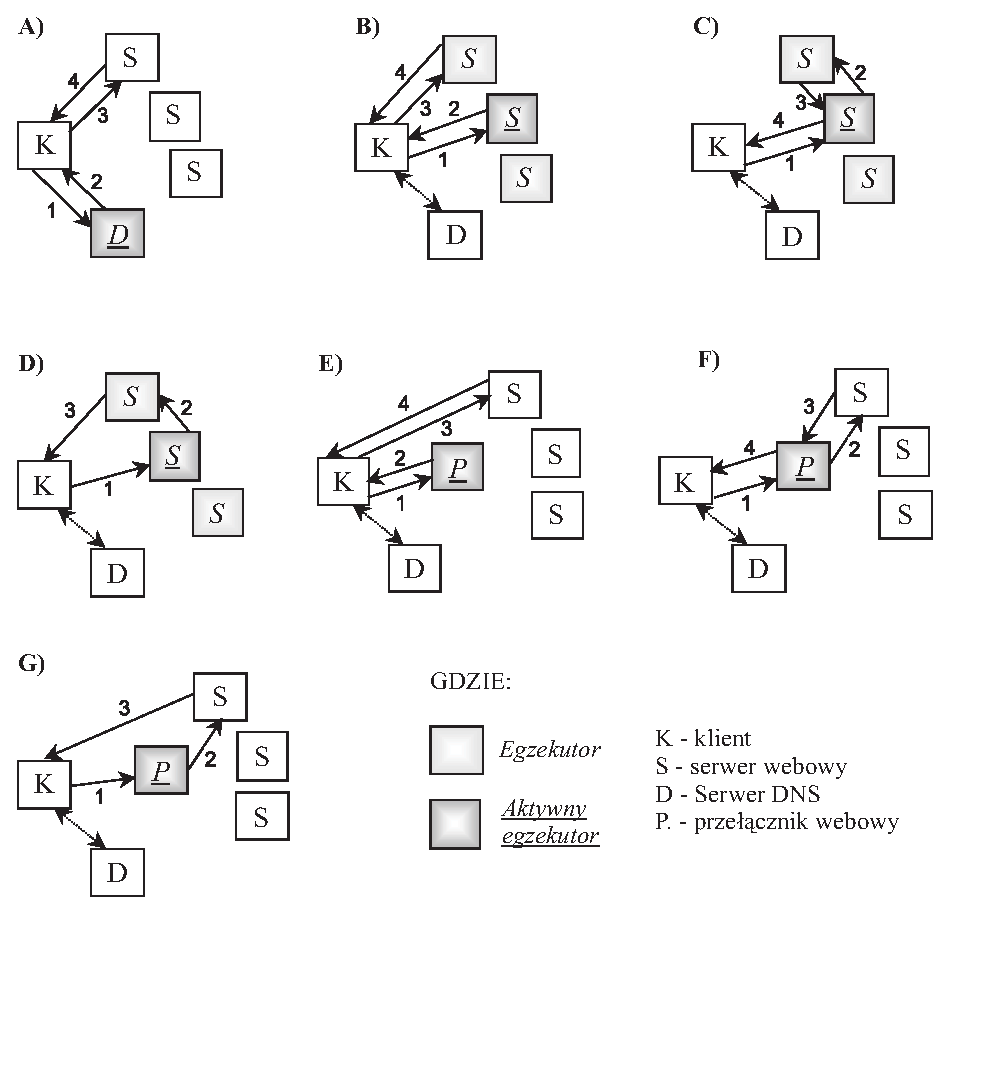
\includegraphics[width=4.9in]{./rysunki/modele_podstawowe.eps}
\caption{Podstawowe modele system�w do r�wnowa�enia obci��e�}
\label{proste_modele}
\end{figure}

\subsection{Podzia� ze wzgl�du na rozmieszczenie serwer�w webowych}
Podzia� ten kszta�tuje si� nast�puj�co:
\begin{itemize}
\item Klaster webowy. Je�li serwery webowe s� rozproszone lokalnie (skupione geograficznie), to m�wi si� o tzw. klastrze 
webowym (web--cluster). Z technicznego punktu widzenia klaster webowy funkcjonuje w obr�bie sieci lokalnej. Ka�dy z prostych 
modeli przedstawionych na rys.\ref{proste_modele} mo�e by� implementowany w klastrze webowym. W przypadku modelu {\bf G}, ze wzgl�du na uwarunkowania 
techniczne transmisji ��da�, mo�e zaj�� potrzeba umiejscowienia klastra w obr�bie podsieci sieci 
lokalnej \cite{modele15,modele20,LoadBalancingWithND}.
\item Rozproszone serwery webowe. Je�li mi�dzy rozproszonymi globalnie (rozproszonymi geograficznie) serwerami webowymi 
stosowany jest jakikolwiek mechanizm szeregowania, m�wi si� o rozproszonych serwerach webowych (distributed web--servers), w 
przeciwnym przypadku -- o lustrzanych serwerach webowych (mirror web--servers). Teoretycznie ka�dy model przedstawiony na rys.\ref{proste_modele}
mo�e by� implementowany w�r�d rozproszonych serwer�w webowych, jednak ze wzgl�du na powstawanie dodatkowych op�nie� podczas 
transmisji zwrotnej w modelu {\bf F} oraz uwarunkowania techniczne transmisji ��da� w modelu {\bf G}, oba wymienione modele maj� 
zastosowanie g��wnie klastrach webowych.
\item Rozproszone klastry webowe. Szczeg�lnym przypadkiem rozmieszczenia serwer�w webowych jest kombinacja globalnego i 
lokalnego rozproszenia. Je�li miedzy klastrami webowymi stosowany jest jakikolwiek mechanizm szeregowania, m�wi si� o 
rozproszonych klastrach webowych (distributed web--clusters). W przeciwnym przypadku -- o lustrzanych klastrach webowych (mirror 
web--clusters). Rozproszone klastry webowe mo�na przedstawia� za pomoc� kombinacji prostych modeli funkcjonalnych (rys.\ref{complex_modele} {\bf J, K}). 
\end{itemize}

\subsection{Podzia� i charakterystyka ze wzgl�du na umiejscowienie mechanizmu szeregowania}

Mechanizm szeregowania mo�e by� umiejscowiony: po stronie klienta, po stronie serwera, oraz jako osobny uk�adu (serwer DNS,
dystrybutor).

\subsubsection{Podej�cie od strony klienta}

G��wn� zalet� stosowania mechanizm�w rozpraszania obci��enia po stronie klienta jest ca�kowita niezale�no�� od architektury 
serwera(�w), a przede wszystkim od miejsca ich rozmieszczenia (mog� by� nie tyle geograficznie rozproszone, co wr�cz 
nieskoordynowane jako ca�o��). 

Rozwi�zania w tym zakresie mo�emy podzieli� na dwie podgrupy:
\begin{itemize}
\item mechanizmy r�wnowa�enia obci��enia implementowane w przegl�darkach i jako applety Java:
\begin{itemize}
\item w przegl�darkach poprzez API. Przegl�darka mo�e aktywnie pe�ni� role� w dystrybucji zapyta�, pod warunkiem posiadania
informacji na temat adres�w serwer�w WWW. Wtedy, na podstawie zapytania otrzymanego od u�ytkownika, przegl�darka wybiera
serwer do przed�o�enia zapytania. Klasycznym przyk�adem takiego rozwi�zania jest mechanizm LB implementowany w przegl�darkach
firmy Netscape \cite{gliwice16,gliwice17}. Po wygenerowaniu zapytania przez u�ytkownika (tylko do serwera 
www.netscape.com), przegl�darka wybiera liczb� z zakresu od 1 do liczby znanych jej serwer�w i kieruje zapytanie do w�z�a
o adresie www\emph{liczba}.netscape.com. Nie jest to rozwi�zanie interesuj�ce, gdy� liczba serwer�w i adres�w jest na sta�e 
zakodowana w przegl�darce. Poza tym taki spos�b rozdysponowywania ruchu (losowy) nie zapewnia r�wnowa�enia obci��enia pomi�dzy
serwerami;
\item applety Java. O wiele ciekawszym od powy�szego rozwi�zaniem, jest implementacja specyficznych applet�w Java. Gdy
u�ytkownik wysy�a ��danie do serwisu, zamiast dokumentu HTML, pobiera applet Java. Applet ten zawiera adresy IP maszyn 
dostarczaj�cych ten serwis WWW \cite{gliwice18,gliwice19}. Applet mo�e by� modyfikowany przez program zbieraj�cy informacje o 
stanie serwer�w (o ich obci��eniu) oraz o jako�ci po��czenia sieciowego. Informacje te mo�e wykorzystywa� applet do
wyboru najbardziej odpowiedniego serwera do realizacji ��dania. G��wn� wad� tego rozwi�zanie jest generowanie 
dodatkowego ruchu w sieci (zwi�zanej z pobieraniem informacji o stanie obci��enia serwer�w. Naturalnie jest ono r�wnie� 
bezu�yteczne gdy przegl�darka nie potrafi interpretowa� kodu Javy.
\end{itemize}
\item serwery Proxy. Jest to oparte na pomy�le po raz pierwszy wykorzystanym przez badaczy z Cambridge 
University \cite{gliwice20}. Mechanizm, kt�ry zosta� zaimplementowany w serwer proxy, bazuje na informacji o 
osi�gni�tej wydajno�ci podczas dotychczasowych transmisji. Klient otrzymuje list� zreplikowanych serwer�w postrzeganych przez
u�ytkownika pod jednym adresem. Ka�dej pozycji na li�cie jest przypisana informacja o wydajno�ci serwera. Za ka�dym razem, 
gdy klient utworzy po��czenie z serwerem jest ona aktualizowana. Wybierany jest mirror na podstawie znajomo�ci
najlepszej ze �rednich wydajno�ci serwera w ci�gu ostatnich transmisji. Decyzja jest podejmowana z zastrze�eniami: je�li 
wydajno�� ostatniej transmisji spad�a poni�ej pewnego progu, serwer jest uwa�any za nieosi�galny. Wyb�r serwera proxy
wynika� z kilku wa�nych powod�w: ukrycie przed u�ytkownikiem faktu wyboru dokumentu mi�dzy zreplikowanymi serwerami, brak
konieczno�ci ingerencji w kod przegl�darki, oraz korzy�� w postaci wsp�dzielenia informacji o wydajno�ci zreplikowanych 
serwer�w mi�dzy u�ytkownikami przegl�darek. Kilku klient�w generuje wi�ksz� liczb� zapyta�, poprawiaj�c w ten spos�b wydajno��
algorytmu r�wnowa�enia obci��enia \cite{gliwice20}. 
\end{itemize}

\subsubsection{Podej�cie od strony serwera}

Techniki r�wnowa��ce obci��enie w oparciu o serwery wykorzystuj� dwupoziomowy mechanizm dystrybucji. Najpierw zapytania
klienta s� przydzielane serwerom webowy w klastrze poprzez DNS. Nast�pnie ka�dy serwer mo�e przekaza� otrzymane zapytanie
do innego serwera w klastrze. Rozwi�zanie w oparciu o rozproszone szeregowanie pozwala wszystkim serwerom bra� udzia�
w r�wnowa�eniu obci��enia w klastrze poprzez mechanizm przekazywania zapyta�. Po��czenie podej�cia w oparciu o DNS oraz z
technikami przekierowywania zapyta� poprzez serwery webowe prowadzi do rozwi�zania wi�kszo�ci problem�w wynikaj�cych z polityki
szeregowania np.: niejednolita dystrybucja zapyta� wewn�trz domeny, czy ograniczona kontrola nad zapytaniami.

Propozycje oparte na przekierowaniach serwer�w r�ni� si� w sposobie podejmowania decyzji. W nast�pnym rozdziale s� 
przedstawione dwie g��wne klasy rozwi�za�: wykorzystuj�ce funkcje redirekcji na poziomie protoko�u HTTP oraz w oparciu o
mechanizm przepisywania pakiet�w. 

\subsubsection{Podej�cie od strony niezale�nego w�z�a dystrybuuj�cego zapytania}

W wyniku zapytania klienta o dane z serwera WWW -- w pierwszej kolejno�ci nast�puje rozwini�cie nazwy domenowej serwera na
jego adres IP. Nast�pnie adres IP mo�e by� reprezentowany przez wirtualny adres IP przypisany do klastra serwer�w. Samo
rozwini�cie IP w adres serwera mo�e by� realizowane na r�nych poziomach. Mo�e to by� przekierowanie do konkretnych zasob�w na 
poziomie protoko�u HTTP \cite{modele2} lub na poziomie protoko�u IP oraz adresu URL przy zastosowaniu 
dystrybutora \cite{modele1,gliwice3}.

Na pocz�tku skupiano si� na rozwi�zaniach dotycz�cych podmiany nazwy serwisu na jego adres IP \cite{gliwice4}. Jednak�e w 
zwi�zku z faktem ogranicze� takiego rozwi�zania coraz wi�ksz� uwag� po�wi�ca si� implementacji mechanizm�w podmiany 
wirtualnego adresu IP na adres konkretnego hosta. Przyk�adami takiego podej�cia s�: Berkeley MagicRouter \cite{modele1}, 
CISCO Local Director \cite{gliwice13}, VirtualServer \cite{virtualserver} oraz IBM SecureWay Network Dispatcher \cite{GettingStarted}.

\begin{itemize}
\item Wykorzystanie serwera DNS -- 
egzekutorem jest serwer DNS lub inne urz�dzenie wspomagaj�ce albo przejmuj�ce rol� serwera DNS. Nale�y u�ci�li�, 
�e chodzi tu o tzw. g��wny serwer DNS b�d�cy autorytatywnym �r�d�em informacji o okre�lonej domenie (\emph{authoritative DNS}).
Jak opisano w Rozdziale 2 system DNS s�u�y do odwzorowania symbolicznych nazw komputer�w w Internecie na ich 
adresy IP. Funkcja ta, w niejako naturalny spos�b, czyni serwer DNS dobrym miejscem na implementacj� mechanizmu 
r�wnowa�enia obci��e�. Pierwsz� instalacj� wykorzystuj�c�  DNS do r�wnowa�enia obci��e� by� serwis WWW NCSA 
(ang. \emph{National Center for Supercomputing Applications}). Zestawiono tam klaster dziewi�ciu serwer�w WWW, kt�ry 
stanowi� odr�bny obszar DNS i by� udost�pniany pod nazw� www.ncsa.ninc.edu \cite{barylo28,barylo29}. Na podstawowym serwerze 
DNS  domeny (obszaru) ncsa.ninc.edu skonfigurowano oprogramowanie, kt�re na zapytania o odwzorowanie nazwy 
www.ncsa.ninc.edu odpowiada�o podaj�c cyklicznie adresy kolejnych serwer�w z klastera. Ten statyczny algorytm 
nazywany jest cyklicznym DNS lub RR--DNS (ang. \emph{Round--Robin DNS}). 

Podej�cie to jednak bardziej realizuje rozproszenie strumienia zapyta� klient�w ni� r�wnowa�enie obci��enia serwer�w WWW. W
rzeczywisto�ci w Internecie jest wiele serwer�w DNA i maj� one uk�ad hierarchiczny tzn. nie zawsze trzeba sprawdza� adres IP
w docelowym serwerze DNS. Oznacza to, �e nie mamy wp�ywu na cz�� zapyta�, jakie s� kierowane do serwera. W pewnym stopniu
poprawia sytuacj� zastosowanie sygna��w zwrotnych od serwera WWW do serwera DNS o przeci��eniu. Efekt jest odczuwalny dopiero 
po up�ywie czasu TTL (np. w momencie uszkodzenia maszyny i wy��czenia jej adresu z puli adres�w serwera DNS). Aby efektywno��
tego typu rozwi�za� by�a jak najwi�ksza, wa�ne jest prawid�owe oszacowanie tzw. ukrytego obci��enia, czyli wielko�ci zapyta�
nap�ywaj�cego w czasie TTL. Do estymowania tej wielko�ci mo�na zastosowa� funkcje heurystyczne \cite{gliwice4}.

\item Reverse proxy serwer

Typowe forward proxy (tak�e transparent) zwykle u�ywane przez prowajder�w internetu przechowuj� strony najcz�ciej pobierane 
przez u�ytkownik�w. Z reverse proxy firmy mog� przechowywa� specyficzn� zawarto�� na 
serwerach podobnie jak prowajderzy i przekierowywa� ��dania (od klient�w) do danych sk�adowanych na tych serwerach poprzez 
proxy. Serwery 
proxy przechowuj� (keszuj�) informacje przychodz�ce od lokalnych serwer�w. Zatem osi�ganie stron jest o wiele szybsze -- jest 
pobierane (o ile istnieje) z keszu serwera proxy (st�d nazwa reverse -- poniewa� jego dzia�anie jest dok�adnie przeciwne do 
dzia�ania ,,zwyk�ego'' proxy serwera). 

Z technicznego punktu widzenia reverse proxy r�ni si� od forward proxy jednym dodatkiem -- tym dodatkiem jest odpowiedni modu� 
t�umacz�cy adresy URL backendowych serwer�w WWW tak jakby by�y to jego w�asne. Taki spos�b dzia�ania ma jeszcze jedn� ciekaw� 
w�asno�� -- serwery backendowe mog� by� specjalizowane, np. niekt�re z nich mog� odpowiada� wy��cznie za przetwarzanie stron 
dynamicznych, inne statycznych, a jeszcze inne tylko stron zawieraj�cych sporo grafik. Wystarczy w module przeadresowa� 
umie�ci� odpowiedni� informacj� (tzn. jaki adres URL w sieci wewn�trznej ,,t�umaczy�'' na adres URL serwera proxy).

W zwi�zku z prostot� dzia�ania takiego systemu (znakomicie wykorzystywanego jako systemu zarz�dzaj�cego wielokomputerow� 
witryn� WWW -- mo�na r�wnowa�y� obci��enia, specjalizowa� serwery, oraz w dowolny spos�b propagowa� ruch webowy) jest on cz�sto 
wykorzystywany. 

Oferta r�norakich produkt�w pe�ni�cych rol� reverse proxy serwer�w jest bardzo bogata. Rozpo�ciera si� od produkt�w 
komercyjnych, takich jak Intel NetStructure, IBM Web Traffic Express (bed�cy elementem WebSphere Edge Server), po produkty 
niekomercyjne takie jak: Apache (najpopularniejszy serwer WWW -- mo�e by� r�wnie� forward, transparent oraz reverse proxy 
serwerem, niestety na razie obs�uguje jedynie protok� HTTP do wersji 1.0), oraz bardzo wydajne narz�dzie: SQUID Web Proxy 
Cache\footnote{http://www.squid--cache.org} (obs�uguj�cy wszystkie wersje protoko�u HTTP, maj�cy te� niezliczon� ilo�� funkcji 
dotycz�cych korzystania z tego systemu i bezpiecze�stwa).

\item Wykorzystanie dystrybutora -- wyspecjalizowanego urz�dzenia.
Alternatywnym rozwi�zaniem do DNS'a, pozwalaj�cym na pe�n� kontrol� ilo�ci zapyta� nadchodz�cych do serwer�w, jest 
zastosowanie dystrybutora. Rozszerza to wirtualizacj� adresu nie tylko na poziom URL, ale r�wnie� na poziom protoko�u IP. 
Dzi�ki temu mo�na zastosowa� jeden wirtualny adres IP (single virtual IP address) IP--SVA dla klastra serwer�w. Pozwala to na 
pe�n� kontrol� nad strumieniem zapyta� kierowanych do serwer�w.

Takie podej�cie ma jednak swoje wady. W systemie powstaje jeden w�ze� obs�uguj�cy transmisj� pakiet�w. W pewnych przypadkach 
wydajno�� ca�ego systemu mo�e zale�e� od wydajno�ci tego w�a�nie w�z�a. Wykorzystywane tutaj algorytmy s� najprostsze, 
poniewa� dystrybutor obs�uguje wszystkie nadchodz�ce pakiety i konieczne jest zminimalizowanie czasu po�wi�canego na ich 
obs�ug�. Przyk�adem takiego rozwi�zania jest SITA-V algorytm  \cite{gliwice10}.

Rozwi�zania oparte na dystrybutorze ze wzgl�du na zastosowany mechanizm obs�ugi pakiet�w mo�emy podzieli� na:
\begin{itemize}
\item metod� packet single--rewriting; rozwi�zanie to polega na przekierowywaniu pakiet�w nadchodz�cych od klient�w przez 
dystrybutor poprzez przepisanie docelowego adresu IP. Przyk�adem takiego rozwi�zania jest mechanizm routera TCP opisany 
w  \cite{gliwice11}. Klaster serwer�w WWW sk�ada si� z kilku w�z��w oraz routera TCP, kt�ry pe�ni rol� dystrybutora.
Adres \emph{i} jest prywatnym adresem w�z�a, na kt�rym uruchomiony jest serwer WWW. Wszystkie zapytania HTTP przychodz� do 
dystrybutora, poniewa� tylko IP--SVA jest adresem znanym publicznie (krok 1). Wyb�r serwera WWW dokonywany jest przez 
dystrybutor na podstawie algorytmu round--robin (krok 2). Przekierowanie pakietu do odpowiedniego serwera realizowane jest
dzi�ki przepisaniu adresu docelowego w pakiecie z IP--SVA na prywatny adres \emph{i} serwera w klastrze. Przepisywana jest 
r�wnie� suma kontrolna w pakiecie, poniewa� zale�y ona od adresu docelowego (krok 3). W zwi�zku z tym, �e jedno ��danie sk�ada 
si� z kilku pakiet�w, dystrybutor przechowuje tablic� z�o�on� z par: adres �r�d�owy -- adres prywatny serwera WWW. Dzi�ki temu 
wszystkie pakiety pochodz�ce od jednego nadawcy mog� by� kierowane do tego samego serwera WWW (krok 4). W nast�pnym kroku 
serwer odsy�a ��dane dane do klienta (krok 6). Przed odes�aniem danych w pakiecie konieczne jest wpisanie w polu adresu 
nadawcy, adresu IP-SVA (krok 5).

Jakkolwiek rozwi�zanie to jest przezroczyste dla klienta, to wymaga ono du�ych zmian w kodzie routera oraz systemie 
operacyjnym serwera. Zwi�zane jest to z tym, �e nast�puje podmiana adres�w na poziomie TCP/IP. Z drugiej jednak strony 
rozwi�zanie to jest bardzo odporne na uszkodzenia. W przypadku awarii serwera WWW jest on usuwany z tablicy routera i nie 
uwzgl�dniany przy rozdziale pakiet�w a� do momentu naprawy. Architektura ta mo�e by� po��czona z wykorzystaniem DNS'a. Pozwala 
to na skalowanie klastra nie tylko w sieci LAN, ale r�wnie� sieci WAN.
\item metod� packet double--rewriting; architektura ta w swoim za�o�eniu jest bardzo podobna do przedstawionej powy�ej. 
Mechanizm polega na przepisywaniu adres�w docelowych w pakietach nadchodz�cych od klient�w. Dystrybutor nast�pnie przesy�a 
pakiety do odpowiedniego w�z�a obs�uguj�cego serwer WWW. W tym przypadku jednak wszystkie pakiety wracaj� z powrotem do 
dystrybutora. Mechanizm ten opiera si� na architekturze NAT (Network Address Translation) opisanej w  \cite{modele17}.
W momencie odebrania nadchodz�cego pakietu dystrybutor wybiera serwer WWW (krok 2), a nast�pnie modyfikuje adres �r�d�owy oraz 
docelowy w nag��wku pakietu (krok 3). W drodze powrotnej pakietu dystrybutor ponownie zmienia adresy IP w nag��wku i przesy�a 
dalej dane do klienta (krok 6). 

Znane s� dwa rozwi�zania oparte na tej architekturze. CISCO LocalDirector  \cite{gliwice13} oraz Magicrouter  \cite{modele1}
\item metod� packet forwarding by the dispatcher.
Packet forwarding jest podej�ciem odmiennym w stosunku do prezentowanych powy�ej. Dzia�anie jego polega na przesy�aniu 
pakiet�w do serwera w niezmienionej postaci zamiast przepisywaniu adres�w w nag��wku. Podej�cie to pozwala na wykorzystanie 
tego samego rozwi�zania w sieci LAN i WAN. Zar�wno sama metoda jak i pakiet zosta�y opisane w dalszej cz�ci tej pracy.
\end{itemize}
\end{itemize}

\subsection{Podzia� ze wzgl�du na strategi� rozmieszczenia mechanizm�w szeregowania}
Z tej perspektywy rysuje si� podzia� na dwie grupy modeli: z centralnym mechanizmem szeregowania i z rozproszonymi 
mechanizmami szeregowania.
\begin{itemize}
\item Centralny mechanizm szeregowania. Do tej grupy nale�� modele {\bf A, E, F, G} (rys.\ref{proste_modele}). W przypadku {\bf A} decyzja o przydzieleniu 
nazwie domenowej adresu IP najlepszego serwera webowego zapada centralnie, po stronie serwera DNS. Mimo scentralizowanego 
zarz�dzania, ze wzgl�du na specyfik� funkcjonowania DNS, skuteczno�� tego modelu jest 
niewielka \cite{modele14,ModeleFunkcjonalne}. W modelach  
decyzja o przekierowaniu ��dania klienta zapada centralnie, w dedykowanym urz�dzeniu. W odr�nieniu od modelu, centralne 
zarz�dzanie oznacza stuprocentow� kontrol� nad szeregowaniem.
\item Rozproszone mechanizmy szeregowania. W tej grupie decyzja o przekierowaniu ��dania mo�e zapa�� na ka�dym serwerze, w 
kt�rym zaimplementowano oprogramowanie egzekutora. Ide� rozproszonego szeregowania ukazuj� modele {\bf B, D, C} (rys.\ref{proste_modele}). Rozwi�zanie takie zapobiega 
efektowi w�skiego gard�a, na kt�re w szczeg�lno�ci nara�ony jest model {\bf F}. Modele {\bf B} oraz {\bf D}
stosowane s� g��wnie w celu poprawy skuteczno�ci szeregowania w modelu {\bf A} (rys.\ref{complex_modele} {\bf H, I}).
\end{itemize}

\subsection{Podzia� ze wzgl�du na liczb� stopni szeregowania}
Systemy serwer�w webowych mog� jednocze�nie wykorzystywa� jeden lub wi�cej mechanizm�w szeregowania. M�wi si� w�wczas o 
skalowalnych systemach serwer�w webowych z szeregowaniem jednostopniowym, dwustopniowym lub tr�jstopniowym. Nie spotyka si� 
system�w o wi�kszej ilo�ci stopni szeregowania. Modele system�w z szeregowaniem wielostopniowym mo�na budowa� poprzez z�o�enie 
modeli prostych. Przyk�adowe modele z�o�one zosta�y przedstawione na rys.\ref{complex_modele}.

\begin{figure}[h]
\centering
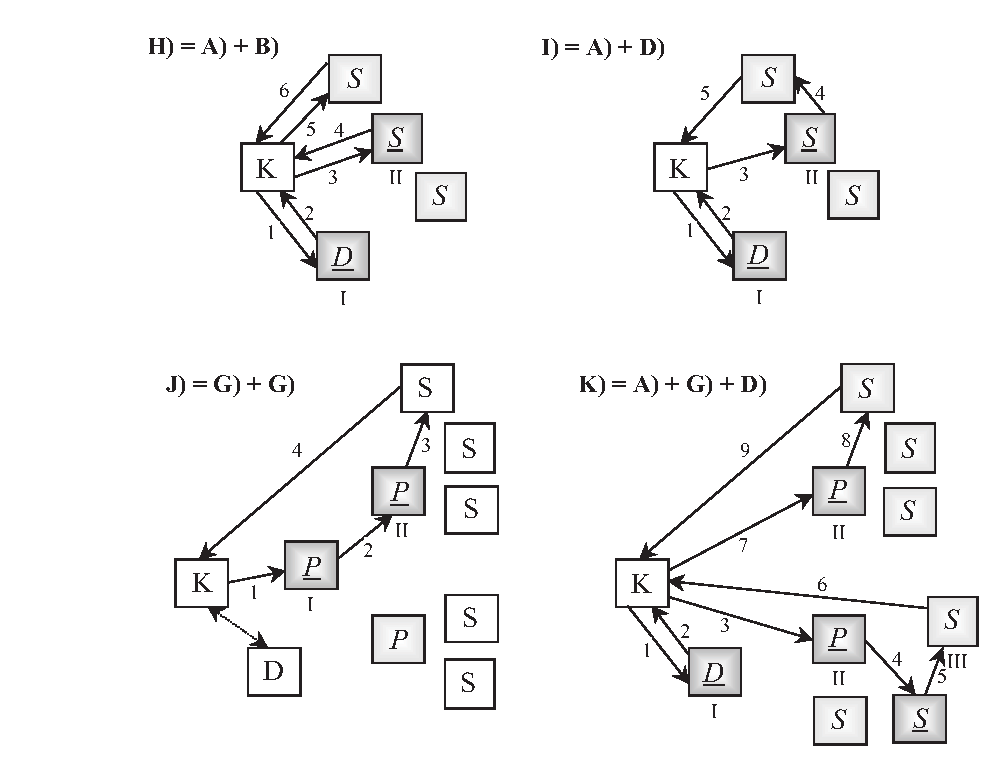
\includegraphics[width=4.9in]{./rysunki/complex_models.eps}
\caption{Z�o�one modele system�w do r�wnowa�enia obci��e�}
\label{complex_modele}
\end{figure}

\begin{itemize}
\item Systemy z szeregowaniem jednostopniowym. Systemy z szeregowaniem jednostopniowym odzwierciedlaj� modele: {\bf A, E, F, G} (rys.\ref{proste_modele}). 
W modelu {\bf A} egzekutor zintegrowany jest z serwerem DNS, natomiast w modelach{\bf E, F, G} rol� egzekutora pe�ni dystrybutor 
lub prze��cznik webowy.
\item Systemy z szeregowaniem dwustopniowym. Przyk�adowe systemy z szeregowaniem dwustopniowym obrazuj� modele {\bf H, I, J} (rys.\ref{complex_modele}).
W przypadku {\bf H} oraz {\bf I} \cite{modele2,modele10,modele23,modele3} na pierwszym stopniu wykorzystywany jest model {\bf A}, natomiast na drugim, odpowiednio 
model {\bf B} lub {\bf D}. W obu przypadkach na pierwszym stopniu egzekutor zintegrowany jest serwerem DNS, natomiast na drugim rol� 
egzekutora pe�ni ten z serwer�w webowych, kt�ry zosta� wytypowany na poziomie serwera DNS. Przypadek {\bf J} ukazuje kaskadowe 
z�o�enie modeli {\bf G} (rys.\ref{complex_modele}) w celu szeregowania ��da� w systemie rozproszonych klastr�w webowych \cite{NDUsersGuide}. Na obu stopniach rol� egzekutora 
mo�e pe�ni� dystrybutor lub prze��cznik webowy. Model ten charakteryzuje si� kr�tk� drog� zapyta�, jednak awaria pierwszego 
stopnia szeregowania unieruchamia ca�y system rozproszonych klastr�w.
\item Systemy z szeregowaniem tr�jstopniowym. Przyk�ad systemu z szeregowaniem tr�jstopniowym pokazuje model {\bf K} \cite{modele9}. Jest to 
system rozproszonych klastr�w webowych, gdzie ka�dy z serwer�w w klastrze ma wbudowany mechanizm szeregowania. Na pierwszym 
stopniu szeregowania wykorzystywany jest model {\bf A}, na drugim model {\bf G}, a na trzecim model {\bf B}, czyli na pierwszym stopniu 
egzekutor zintegrowany jest z serwerem DNS, na drugim role egzekutora pe�ni dystrybutor lub prze��cznik webowy, natomiast na 
trzecim ten serwer webowy, kt�ry zosta� wytypowany przez egzekutor na drugim stopniu. Ka�dorazowe zadzia�anie trzeciego 
stopnia szeregowania, mo�e powodowa� znaczne op�nienia, jednak model ten jest bardzo odporny na przeci��enia i awarie. 
\end{itemize}

\subsection{Podzia� ze wzgl�du na poziom szczeg�owo�ci szeregowania}

\subsubsection{Szeregowanie na poziomie serii ��da� o strony}
Aby zrealizowa� ��danie klienta o stron� umiejscowion� pod pewn� nazw� domenow�, mechanizm szeregowania, kt�ry jest 
zintegrowany z serwerem DNS, musi przydzieli� tej nazwie adres IP najlepszego serwera webowego (hostname resolution). Ze 
wzgl�du na du�� bezw�adno�� DNS kolejne ��dania klienta o strony umiejscowione pod t� nazw� domenow� b�d� przez pewien czas 
kierowane do tego samego serwera webowego. Przypadek, w kt�rym szeregowanie ��da� klient�w odbywa si� na poziomie serii ��da� 
o strony, przedstawia model {\bf A}. 

\subsubsection{Szeregowanie na poziomie ��dania o stron�}
W sk�ad strony webowej wchodzi zwykle wiele obiekt�w. Na tym poziomie przekierowanie ��dania o stron� poci�ga za sob� 
przekierowanie serii ��da� o jej elementy sk�adowe. Mechanizm szeregowania wykorzystuje w tym celu w�a�ciwo�ci protoko�u HTTP 
(HTTP redirection \cite{modele18}). Przypadki, w kt�rych wyst�puje tego typu szeregowanie, ukazuje model {\bf B} oraz {\bf E}. W przypadku modelu {\bf B}, gdy jeden 
z serwer�w webowych otrzymuje od klienta ��danie o stron�, je�li nie decyduje si� sam zrealizowa� zlecenia, 
odsy�a klientowi adres IP lub nazw� domenow� lepszego od siebie serwera \cite{modele23}. W przypadku modelu {\bf E}, gdy prze��cznik otrzymuje 
od klienta ��danie o stron�, odsy�a mu adres IP lub nazw� domenow� najlepszego serwera \cite{modele19}. 
Nale�y zaznaczy�, �e mo�e wyst�pi� tu zjawisko buforowania przez klienta adresu IP serwera, do kt�rego nast�pi�o 
przekierowanie. Mo�na w�wczas m�wi� o szeregowaniu na poziomie serii ��da� o strony.

\subsubsection{Szeregowanie na poziomie ��dania o obiekt}
Przypadki, w kt�rych szeregowanie odbywa si� na poziomie ��dania o obiekt, przedstawiaj� modele {\bf C, D, F} oraz {\bf G}. W tej grupie 
mechanizm szeregowania zajmuje si� przekierowywaniem pakiet�w (packet redirection). Pakiety zawieraj�ce ��danie o obiekt musz�
w komplecie trafi� do wybranego przez egzekutor serwera. Jednym ze sposob�w realizuj�cych ten cel jest zapisywanie wynik�w 
decyzji egzekutora w tzw. tablicy powi�za� (binding table).
Poniewa� w modelu {\bf D} ruch pakiet�w powracaj�cych (znacznie 
wi�kszy ni� w przypadku pakiet�w z ��daniami) jest kierowany do klienta z pomini�ciem serwera-egzekutora, model ten jest z 
powodzeniem implementowany. Charakterystyczn� cech� modeli {\bf F, G} jest to, �e egzekutor maskuje serwery webowe za pomoc� 
jednego, wirtualnego adresu IP-SVA (single virtual IP address). Aby przekaza� ��danie do konkretnego serwera, stosuje r�ne, 
niekiedy wyrafinowane techniki. Gdy egzekutor przekierowuje pakiety z ��daniami bez �wiadomo�ci ich tre�ci (content 
information blind), nazywany jest dystrybutorem (dispatcher, level 4 web-switch). Gdy egzekutor podczas podejmowania decyzji o 
przekierowaniu wykorzystuje informacj� zawart� w ��daniu (content information aware), nazywany jest prze��cznikiem webowym 
(content switch, level 7 web-switch).
Nale�y podkre�li�, �e niniejszy podzia� dotyczy wariantu, gdzie w modelach {\bf F, G} rol� egzekutora pe�ni dystrybutor. 
W przypadku gdy egzekutorem jest prze��cznik webowy, szeregowanie mo�e odbywa� si� na poziomie ��dania o obiekt, stron� oraz 
(dzi�ki umiej�tno�ci rozpoznawania znacznik�w cookie) serii ��da� o strony.

\subsection{Podzia� ze wzgl�du na poziom kontroli zapyta�}
Jest to podzia� wyodr�bniaj�cy modele, w kt�rych egzekutory maj� pe�na kontrol� nad zapytaniami kierowanymi do systemu 
serwer�w webowych.
\begin{itemize}
\item Pe�na kontrola zapyta�. Teoretycznie do tej grupy nale�� modele {\bf B, C, D, E, F} i {\bf G}. Klient, po otrzymaniu od 
serwera DNS adresu IP egzekutora, wszystkie zapytania kieruje tylko i wy��cznie do niego. W ten spos�b egzekutor ma 
stuprocentow� kontrol� nad zapytaniami. W rzeczywisto�ci sytuacja taka zachodzi w przypadku modeli {\bf F} oraz {\bf G}. Warto zwr�ci� 
uwag�, �e awaria lub zapchanie si� egzekutora powoduje unieruchomienie ca�ego systemu serwer�w webowych. 
\item Cz�ciowa kontrola zapyta�. Typowym przypadkiem, w kt�rym egzekutor sprawuje cz�ciow� kontrol� nad zapytaniami, jest 
model {\bf A}. Cz�ciowa kontrola wynika ze specyfiki funkcjonowania systemu DNS. R�wnie� modele {\bf B, E} nale�y zaliczy� do tej 
grupy ze wzgl�du na mo�liwo�� wyst�powania zjawiska buforowania przez klienta adresu IP serwera, do kt�rego nast�pi�o 
przekierowanie. Je�li modele {\bf C} i {\bf D} by�yby implementowane samodzielnie, egzekutor, kt�rego adres IP rozg�asza�by serwer 
DNS, sprawowa�by pe�n� kontrole nad zapytaniami. Jednak w przypadku modelu {\bf D} typowym rozwi�zaniem jest jego z�o�enie z 
modelem {\bf A} (model {\bf I} rys.\ref{complex_modele}). W takim przypadku ka�dy z egzekutor�w implementowanych w serwerach webowych sprawuje cz�ciow� 
kontrol� nad zapytaniami kierowanymi do systemu serwer�w webowych.
\end{itemize}

\subsection{Podzia� ze wzgl�du na poziom zaanga�owania egzekutora} 
Egzekutor mo�e by� w r�nym stopniu zaanga�owany w przekierowywanie zapyta� klienta. Mo�e by� r�wnie� zaanga�owany w proces 
przekazywania odpowiedzi. Rysuj� si� tu cztery grupy modeli: bierne, zwrotne, jednokierunkowe oraz dwukierunkowe:
\begin{itemize}
\item Model bierny. Jest to model {\bf A}, w kt�rym do egzekutora w og�le nie trafiaj� ��dania klienta o strony czy obiekty. 
Egzekutor odpowiada tylko na ��dania o prze�o�enie nazwy domenowej na adres IP najlepszego serwera (klastra) webowego, nie 
bior�c bezpo�redniego udzia�u w szeregowaniu zapyta� klienta.
\item Modele zwrotne. Nale�� do nich modele {\bf B, E} (rys.\ref{proste_modele}). Egzekutor, po otrzymaniu ��dania, zwraca klientowi adres IP lub nazw� 
domenow� najlepszego serwera, aby ten m�g� ponowi� ��danie. W modelu {\bf B} mo�e dodatkowo zapa�� decyzja o obs�u�eniu ��dania 
przez bie��cy serwer. Zaanga�owanie egzekutora w proces przekierowywania jest w tym przypadku minimalne.
\item Modele jednokierunkowe. Nale�� do nich modele {\bf D} oraz {\bf G}\cite{modele15,modele20,NDUsersGuide}. ��dania, kt�re osi�gaj� egzekutor, przekierowywane 
s� bezpo�rednio do serwer�w webowych. W modelu {\bf D} mo�e dodatkowo zapa�� decyzja o obs�u�eniu ��dania przez bie��cy serwer. 
Dzi�ki odpowiednim zabiegom technicznym serwery kieruj� odpowiedzi bezpo�rednio do klienta. Zaanga�owanie egzekutora w proces 
przekierowywania jest w tym przypadku �rednie.
\item Modele dwukierunkowe. Nale�� do nich modele {\bf C} i {\bf F} \cite{modele1,modele11,modele17} . Wszystkie ��dania, kt�re osi�gaj� egzekutor, 
przekierowywane s� bezpo�rednio do serwer�w webowych. W modelu {\bf D} mo�e dodatkowo zapa�� decyzja o obs�u�eniu ��dania przez 
bie��cy serwer. Serwery webowe wszystkie odpowiedzi przesy�aj� do egzekutora, kt�ry musi je przekierowywa� do klienta. 
\end{itemize}

\section{Witryny dynamiczne}

\hspace{0.63cm}Ju� nawet kilkudziesi�cioma dokumentami World Wide Web, czyli bardzo niewielkim serwisem, trudno jest zarz�dza�, 
zmienia� i dodawa� nowe fragmenty, czuwa� nad poprawno�ci� dost�pnych w nim danych. Z drugiej jednak strony oprogramowanie 
stosowane do korzystania z World Wide Web jest bardzo proste, szeroko znane i szybko uaktualniane.

Wi�kszo�� informacji zapisanych na komputerach i wykorzystywanych w biznesie czy przez �rodki przekazu zgromadzona jest w 
bazach danych, w tym najcze�ciej w relacyjnych bazach danych. Bazy danych pozwalaj� na kontrol� nad danymi, analizowanie ich, 
ogranizacj� i prezentacj� u�ytkownikowi w jak najbardziej prosty i skuteczny spos�b. Potrzebny jest jednak do nich dostep 
przez wyspecjalizowane oprogramowanie. W systemach klient/serwer jest to klient bazy danych; kolejny program, kt�ry musi 
poznawa� u�ytkownik, program nie zawsze prezentuj�cy najwy�szy poziom mo�liwo�ci technicznych czy �atwo�ci komunikacji z 
u�ytkownikiem.

Oba te systemy, World Wide Web i bazy danych, stworzone s� w tym samym celu -- efektywnego dost�pu do informacji. Ju� po kilku 
latach rozwoju World Wide Web zorientowano si�, �e mo�na je po��czy�, bior�c z ka�dego, co najlepsze. Po��czy� �atwo�� dost�pu,
jak� niesie przegl�darka World Wide Web z wysokim stopniem organizacji oferowanym przez relacyjn� baz� danych.

Sam serwer HTTP nie potrafi si� jednak bezpo�rednio porozumiewa� z baz�; potrzebuje dodatkowego oprogramowania. Dawniej 
najlepsz� metod� nawi�zania kontaktu mi�dzy serwerem HTTP a baz� by�o napisanie programu w standardzie CGI 
\footnote{ang. \emph{Common Gateway Interface}}. Program CGI przyjmuje informacje od serwera HTTP, przetwarza je i 
wysy�a do bazy danych, baza 
danych wykonuje zlecane jej zadanie, wysy�a efekt do programu CGI, kt�ry z kolei zwraca go przez serwer HTTP do klienta HTTP. 
Rezultatem jest najcz�ciej plik HTML. Dzi� mechanizm porozumiewania si� pozostaje taki sam, ale w miejsce programu CGI 
wchodzi program napisany w API serwera HTTP, na przyk�ad ISAPI dla Microsoft Internet Information Server. To drugie 
rozwi�zanie jest bardziej efektywne i pozwala na mniejsze obci��enie komputera, na kt�rym dzia�a serwer, ni� w przypadku 
u�ycia programu CGI.

Mo�na stworzy� serwis World Wide Web, kt�ry porozumiewa si� z baz� danych. Mo�na wpisywa� do bazy nowe informacje, na przyk�ad 
wype�niaj�c ankiet� marketingow�, mo�na przegl�da� istniej�ce informacje, poprawia� je o ile mamy do tego prawo a tak�e 
wyszukwia� potrzebne informacje.

Dok�adnie takie same mo�liwo�ci ma serwis wewn�trzny firmy -- intranetowy. Mo�e on s�u�y� do porozumiewania si� z firm� 
oddzia��w terenowych czy pracownik�w w podr�ach s�u�bowych, a tak�e do zwyk�ej, codziennej komunikacji z baz� danych. 
Przegl�darka World Wide Web jest �atwiejszym w obs�udze i bardziej znanym u�ytkownikom oprogramowaniem ni� specjalny klient 
bazy danych.

Do stworzenia takiego systemu potrzebny jest serwer HTTP i baza danych, a pomi�dzy nimi program po�rednicz�cy. Mo�na napisa� 
w�asne oprogramowanie po�rednicz�ce, ale r�wnie� skorzysta� z gotowych produkt�w.

\section{Testowanie serwer�w WWW}


Jak wiadomo s�aba wydajno�� wprost przek�ada si� 
na niezadowolenia klient�w, a niezadowolony klient opu�ci witryn� Web i
mo�e nigdy ju� na ni� nie wr�ci� \cite{savoia1,savoia2,savoia3}.

Przewidywanie jak witryna WWW b�dzie odpowiada� na specyficzne obci��enie
jest wielkim wyzwaniem. Od czasu jak sajty webowe stanowi� kompleksowe
systemy zawieraj�ce elementy sprz�towe, programowe i sieciowe pochodz�cymi od
r�nych producent�w, oraz posiadaj� bardzo r�ne profile wydajno�ciowe -- 
jest praktycznie niemo�liwa predykcja, jak dany system zachowa si� podczas
obci��enia. Jedynym pewnym sposobem sprawdzenia skalowalno�ci systemu
jest przeprowadzenie test�w wydajno�ciowych, w kt�rych nat�enie i 
charakterystyka przewidywanego ruchu jest symulowana tak realistycznie jak
to jest mo�liwe. 

Testowanie obci��enia witryn webowych stanowi priorytet dla firm robi�cych interesy online. Jak wielu u�ytkownik�w z 
akceptowalnymi czasami odpowiedzi mo�e obs�u�y� strona ? Jest to niezwykle wa�na informacja wykorzystywana do planowania 
kampanii reklamowych, estymacji bud�et�w bran�y IT a nawet do zwyk�ego dostarczania us�ug. I pomimo wagi tego problemu 
praktycznie wi�kszo�� test�w obci��eniowych jest wykonywana niepoprawnie, poniewa� nie odpowiadaj� one rzeczywistym warunkom. 

Poni�ej zostan� opisane elementy, niezb�dne podczas konstrukcji
wysoce realistycznych i dok�adnych test�w wydajno�ciowych sajt�w webowych (znajduj� si� r�wnie� najcz�ciej pope�niane w
typowych testach obci��eniowych b��dy oraz spos�b radzenia sobie z nimi):
\begin{enumerate}
\item Zrozumienie natury obci��enia

Pierwszym krokiem jest dok�adne i obiektywne zrozumienie
natury obci��enia, jakie musi zosta� wygenerowane, podczas symulacji ruchu na witrynie.

Niestety, testowanie obci��enia sajt�w webowych jest dziedzin� ralatywnie
now� (tote� s�abo zrozumian� i udokumentowan�), a do tego jest bardzo ezoteryczn�
dziedzin� test�w. �eby odpowiednio zrozumie� natur� obci��e� nale�y mo�liwie
cz�sto korzysta� z narz�dzia dokonuj�cego analizy log�w naszego web serwera.
Daje to mo�liwo�� obserwacji detali odwiedzin ka�dego u�ytkownika: jego adresu IP, daty i czasu odwiedzin; jakie, 
ile i o jakiej wielko�ci dane pobiera�, czy pobranie by�o zako�czone sukcesem, czy nie oraz inne dane o sesji u�ytkownika, 
jego systemie operacyjnym i narz�dziu z jakiego korzysta�. 

    \begin{description}
    \item[Sesja u�ytkownika -- niezb�dne informacje]\

Wi�kszo�� potrzebnych informacji jakie nale�y wyekstrahowa� podczas analizy log�w s� informacje zwi�zane z sesjami 
u�ytkownik�w\footnote{ang. \emph{user sessions}}. Testy obci��eniowe najbardziej zwi�zane s� w�a�nie z sesjami u�ytkownika. 
Sesj� u�ytkownika definiuje si� jako sekwencj� pobra� stron zwi�zan� z unikatowym (pojedynczym, identyfikowalnym) u�ytkownikiem.

Typowa witryna webowa jest wizytowana przez szerok� gam� u�ytkownik�w z szerok� gam� dzia�a�. Np. u�ytkownicy stron zwi�zanych 
z szeroko rozumianym e--commersem: niekt�rzy z nich przyszli poogl�da� (\emph{browse}), niekt�rzy kupi�, jeszcze inni 
sprawdzi� status
zam�wie�. Nawet je�li grupa klient�w dokonuje pojedynczego dzia�ania, takiego jak kupowanie ksi��ki, ka�dy z tej grupy mo�e to 
realizowa� na szereg sposob�w. Niekt�rzy b�d� porusza� si� ze strony na stron� bardzo szybko, raczej nie dbaj�c o dok�adne 
przeczytanie znajduj�cych si� tam informacji, inni przeciwnie -- poruszaj� si� powoli czytaj�c ka�d� stron� bardzo uwa�nie. 
Niekt�rzy b�d� wyszukiwa� czytaj�c fragmenty wielu ksi��ek zanim zdecyduj� si� na kupno jednej, inni skieruj� si� od razu do 
miejsca zam�wienia \emph{(purchase page)}.

Zrozumienie tej szerokiej gamy akcji, dzia�a� i zachowa� jest niezb�dne (krytyczne) dla zaprojektowania test�w obci��eniowych, 
poniewa� dobrze zaprojektowany test powinien odzwierciedla� zachowania u�ytkownik�w tak precyzyjnie jak to tylko mo�liwe. 
Najlepsz� metod� jest u�ywanie analizator�w log�w (podczas pracy witryny) oraz wydobycie kluczowej grupy zmiennych zachowania 
klient�w najcz�ciej spotykanych na danym sajcie, adekwatnych do ruchu webowego. Niekt�re ze zmiennych, na kt�re zawsze 
powinno zwr�ci� si� uwag� to:
	\begin{itemize}
	\item d�ugo�� trwania sesji (mierzona w stronach);
	\item czas trwania sesji (duration) (mierzona w minutach i sekundach);
	\item typ stron wizytowanych podczas trwania sesji (strona domowa, strona informacji o produkcjie, strona informacji o kartach 
	kredytowych).
	\end{itemize}

Naturalnie nie s� to wszystkie zmienne maj�ce wp�yw na charakterystyk� obci��eniow� sajtu -- opr�cz nich nale�y wybra� jeszcze 
jakie� zmienne kt�re o specyfice danej witryny decyduj�.

Tak� specyfik� mo�na zauwa�y� na przyk�adzie: siedmio--stronicowa sesja, kt�rej rezultatem jest zam�wienie artyku�u znacznie 
bardziej obci��a system ni� siedmiostronicowa sesja, kt�rej wynikiem jest tylko przegl�danie dokument�w. Przegl�danie 
dokument�w jest zwykle zwi�zane z dokumentami statycznymi, za� na sesj�, kt�rej efektem jest dokonanie zakupu artyku�u sk�ada 
si� ca�y szereg czynnik�w takich jak: przeszukiwanie bazy danych zasob�w witryny, u�ytkownika, transakcji kart kredytowych z 
weryfikacj� (osobne systemy), a tak�e wys�anie potwierdzaj�cego zam�wienie e--maila. Statystycznie rzecz bior�c pojedyncza 
sesja zakupu mo�e poch�on�� zasoby sajtu tak jak dwadzie�cia sesji statycznych \emph{(browsing)}. 

W podobny spos�b mo�na por�wna� zakupy dokonywane przez nowych i sta�ych klient�w. Nowy u�ytkownik potrzebuje dokona� 
rejestracji, potwierdzenia i weryfikacji swoich danych, za� sta�y ju� nie. Zwi�zane z baz� danych zak�adanie u�ytkownika mo�e 
by� r�wne obci��eniu generowanemu przez pi�ciu sta�ych u�ytkownik�w, dlatego trzeba wyr�ni� co najmniej dwa typy 
wykorzystania zasob�w przy realizacji zakup�w.

Gdy zostan� ju� zdeterminowane wszystkie zmienne zwi�zane z sesj� u�ytkownika -- nale�y nast�pnie znale�� (zwykle r�wnie� w 
logach) rang� i dystrybucj� warto�ci tych zmiennych np. procentowa (w ca�o�ci ��da�) ilo�� ��danych stron podczas sesji.  Do 
takich cel�w mo�na u�ywa� narz�dzi statystycznych takich jak: odchylenie standardowe, jednak�e najlepszym sposobem 
charakteryzowania wi�kszo�ci zmiennych webowych test�w obci��eniowych jest u�ycie rozproszenia jako warto�ci dyskretnej.

Wielko�� detali i precyzj� z jak� nale�y analizowa� te zmienne zale�y od struktury sajtu (i jej komplikacji), czasu test�w, 
oraz analizy wynik�w. 

    \item[Wsp�bie�ni u�ytkownicy]\

Zazwyczaj w testach obci��eniowych witryn webowych podaje si� warto�ci obci��enia 
spowodowanego naraz wsp�u�ytkuj�cymi zasoby u�ytkownikami. Jednak�e wsp�bie�ni u�ytkownicy nie powinni by� widziani 
jako zmienna wej�ciowa w te�cie, ale jako rezultat wielu r�nych czynnik�w. A zwkle podaje si� np. strona 
zosta�a przetestowana z obci��eniem 1000 wsp�bie�nymi u�ytkownikami. Liczba wsp�bie�nych u�ytkownik�w nie jest miernikiem 
obci��enia. Warto�� ta jest rezultatem wydajno�ci (zdolno�ci do przyj�cia obci��enia) witryny. Efektem pracy na wolniejszym 
sajcie b�dzie wi�ksza liczba wsp�bie�nych u�ytkownik�w. Mo�na to pokaza� na przyk�adzie -- je�li na stron� loguje si� trzech 
u�ytkownik�w w odst�pnie czasowym 1min i pracuj� po 1 min (np. dokonuj� zakup�w) -- to tylko i wy��cznie w zale�no�ci od 
wydajno�ci witryny oraz jej obci��enia b�dzie 0, 2 i 3 naraz pracuj�cych u�ytkownik�w. Zatem je�li wydajno�� witryny webowej z 
jakiego� powodu spada to wzrasta� b�dzie liczba wsp�bie�nych u�ytkownik�w. Trzeba jednak�e doda� jeszcze jeden element -- 
je�li wydajno�� sajtu spada (ro�nie liczba wsp�bie�nych u�ytkownik�w) ro�nie tak�e ilo�� u�ytkownik�w, kt�rzy rezygnuj� z 
korzystania z jego zasob�w. Je�li witryna jest bardzo szybka to mog� si� zdarzy� sytuacje, �e ilo�� wsp�bie�nych u�ytkownik�w 
b�dzie oscylowa� wok� zera (nawet przy ich du�ej ilo�ci). 

Z tych powod�w u�ywanie jako miernika obci��enia strony ilo�ci wsp�pracuj�cych naraz u�ytkownik�w jest (je�li ma by� 
realistyczne) bardzo trudne, a wyniki zawsze odbiegaj� od rzeczywistych. Znacznie lepszym wska�nikiem obci��enia witryny jest 
liczba sesji u�ytkownika wystartowana na godzin�. Ma to wa�n� zalet� -- jest to warto�� sta�a, niezmienna w zale�no�ci od 
wydajno�ci witryny w te�cie. Daje wska�nik ilu u�ytkownik�w otrzyma stron� pierwsz� witryny -- to czy ci u�ytkownicy uko�cz� 
swoj� sesj�, czy nie zale�y ju� od zdolno�ci strony do uniesienia danego obci��enia. I jest to w�a�nie ta warto��, kt�r� si� 
poszukuje podczas wykonywania test�w.

    \item[Rezygnacja klient�w]\

Kolejn� wa�n� wielko�ci�, niejednokrotnie �le szacowan� w testach, a maj�c� znaczny wp�yw na testy obci��eniowe 
witryny jest rezygnacja klient�w w trakcie sesji. U�ytkownicy cz�sto rezygnuj� podczas sesji np. zakup�w z powodu bardzo 
d�ugich odpowiedzi serwera. Zmienn� t� nale�y r�wnie� bra� pod uwag� podczas wykonywania test�w obci��eniowych na 
przygotowywanym 
sajcie. Symulacja porzucania przez u�ytkownik�w sesji powinna by� dokonana tak rzeczywi�cie jak to tylko mo�liwe. Je�li nie, 
podczas test�w b�dzie si� symulowa� obci��enie tak wielkie jakie mo�e nigdy nie nast�pi�, lub w�skie gard�a, kt�re w 
rzeczywisto�ci nigdy si� nie pojawi�. Pominie si� zatem najbardziej istotne wyniki test�w obci��eniowych: czyli 
u�ytkownik�w, kt�rzy mog� porzuci� sesj� z powodu s�abej wydajno�ci. Zatem testy stan� si� nieu�yteczne. W poni�szej 
tabelce znajduj� si� przyk�adowe zale�no�ci pomi�dzy liczb� opuszczaj�cych witryn� u�ytkownik�w, a czasem oczekiwania na 
okre�lon� stron�.
\begin{table}[h]
\centering
\begin{scriptsize}
\begin{tt}
\begin{tabular}{|c|c|c|c|c|}
\hline
{Typ strony}&{\% opuszczaj�cych}&{\% opuszczaj�cych}&{\% opuszczaj�cych}&{\% opuszczaj�cych}\\
{}&{ 0--5 s }&{ 5--10 s }&{ 10--15 s }&{ 10--20 s }\\
\hline\hline
{Strona domowa}&{0\%}&{30\%}&{45\%}&{75\%}\\
\hline
{Stock quote}&{0\%}&{15\%}&{25\%}&{45\%}\\
\hline
{Stock Transaction}&{0\%}&{0\%}&{0\%}&{15\%}\\
\hline
{Account Information}&{0\%}&{5\%}&{15\%}&{35\%}\\
\hline
\end{tabular}
\end{tt}
\caption{�redni stopie� porzucania witryny w \% dla r�nych typ�w stron}
\label{porzucanie}
\end{scriptsize}
\end{table}
Je�li zatem odpowied� oczekiwania na stron� domow� wynosi 5 sek. lub mniej nie obserwuje si� ucieczki klient�w. Jednak�e 
powy�ej tego czasu rezygnacja z oczekiwania staje si� coraz wyra�niejsza, by w czasie 15--20 sek. $3/4$ obecnych na witrynie 
klient�w ju� zrezygnowa�o. Jednak�e nale�y zwr�ci� uwag� na jeszcze jeden zwi�zany z tym szczeg�. Rezygnacja u�ytkownik�w 
zmniejsza obci��enie, zatem wydajno�� zaczyna si� zwi�ksza�, mniej u�ytkownik�w rezygnuje -- a� w ko�cu obci��enie z powrotem 
powoduje oczekiwania na realizacj� ��da� o strony i cykl si� powtarza. Jest to oczywi�cie przyk�ad. Rezygnacja u�ytkownik�w z 
us�ug witryny jest bardzo wa�n� zmienn� pokazuj�c�, �e dany sajt nie jest w stanie satysfakcjonuj�co zapewnia� us�ug przy 
obci��eniu. Najcz�ciej oprogramowanie do testowania potrafi symulowa� rezygnacj� u�ytkownik�w, ale z ekstremalnych powod�w -- 
zwykle 60--120sek. Jednak�e takie warto�ci s� nie do przyj�cia gdy� praktycznie nikt nie czeka tyle czasu. Aby m�c wykona� 
testy obci��eniowe tak prawdopodobne jak to tylko mo�liwe, mo�na skonfigurowa� testowan� witryn� w taki spos�b, aby 
przekierowywa� cz�� u�ytkownik�w na wolniejszy mirror tej witryny. Mo�na np. w ten spos�b: 90\% ruchu jest kierowane na 
zwyk�y serwer, za� 10\% na wolniejszy mirror, na kt�rym np. strona domowa b�dzie serwowana p�niej o 5 sek. W takiej 
konfiguracji nale�y ten dwuserwerowy system uruchomi� na kilka godzin lub dni, do czasu otrzymania znacz�cych wynik�w. Po tym 
czasie nale�y dokona� analizy porzucaj�cych transakcje webowe klient�w. Je�li na zwyk�ym serwerze opuszczanie sesji po stronie 
domowej si�ga 6\%, za� na tym wolniejszym 20\%, trzeba si� liczy� z opuszczaniem witryny przez 14\% klient�w, kt�rzy nie b�d� 
zbyt cierpliwi by poczeka� kolejne 5 sek.

Porzucanie operacji webowych przez klient�w nie jest interesuj�cym wynikiem, samym w sobie -- daje pogl�d na to jakie cz�ci 
sajtu s� najbardziej obci��one w warunkach pracy. Je�li np. strona domowa jest wyj�tkowo wolna, wi�kszo�� u�ytkownik�w nawet 
nie rozpocznie sesji. Wida� zatem, �e odpowiednie symulowanie tego parametru jest bardzo istotne dla stworzenia wydajnego 
sajtu.

    \item[Dystrybucja zapyta� o stron�]\

Kolejn� wa�n� zmienn�, kt�rej warto po�wi�� uwag� jest dystrybucja zapyta� o  stron�. Ta wa�na warto�� okre�la o jakie strony 
s� zapytania i w jakich proporcjach. Procedura zbierania tej danej jest dwustopniowa: najpierw nale�y zdefiniowa� 
skategoryzowane grupy stron, a nast�pnie obliczy� udzia� procentowy ��da� o strony w ka�dej grupie. 

    \end{description}

\item Estymacja wzrostu ruchu na witrynie

Kolejnym krokiem przy projektowaniu test�w obci��eniowych jest zrozumienie pewnych kluczowych zmiennych -- niezb�dnych do 
estymowania docelowego poziomu obci��enia:
    \begin{itemize}
    \item jak wzrasta ca�kowite obci��enie ruchu na sajcie;
    \item jaki jest poziom obci��enia pojedynczych pik�w, maj�cych wp�yw w ca�kowitym obci��eniu;
    \item jak szybko liczba u�ytkownik�w mo�e wp�yn�� na osi�gni�cie maksimum piku obci��eniowego;
    \item jak d�ugo trwaj� poszczeg�lne piki.
    \end{itemize}

Przy pomiarze poziomu obci��enia mo�na u�ywa� zmiennej: liczba sesji u�ytkownik�w na jednostk� czasu. Taki wyb�r wynika z jego 
prostoty w zrozumieniu i �atwo�ci analizy.

    \begin{description}
    \item[Estymacja przysz�ego ruchu webowego]\

Ocena szybko�ci wzrostu ca�kowitego obci��enia ruchu jest istotna, poniewa� rozmiar poziomu pik�w jest 
proporcjonalny do amplitudy ca�kowitego ruchu. Je�li ca�kowity ruch wynosi np. 100000 sesji na tydzie�, oznacza to piki o 
wielko�ci 1500 sesji na godzin�, zatem przy obci��eniu rz�du 200000 sesji na tydzie� piki (chwilowe obci��enia) mog� si�ga� 
3000 sesji na godzin�. 

Ca�kowity wzrost wielko�ci ruchu wynika z dw�ch czynnik�w: danych historycznych (o wzro�cie) oraz szacunk�w 
sprzeda�y/marketingu. Aby estymowa� te warto�ci, nale�y dokona� analizy tygodniowego ruchu oraz dowiedzie� si� od odpowiednich 
ludzi w firmie jak mo�e si� zmienia� ruch z miesi�ca na miesi�c, oraz jak mo�e wygl�da� zainteresowanie na witrynie po 
specjalnych ofertach marketingowych. Z takich informacji mo�na oszacowa� warto�� obci��enia w czasie -- czyli przysz�e 
mo�liwo�ci sajtu. 

    \item[Estymacja ruchu chwilowego]\

Po dokonaniu analizy wzrostu ca�kowitego obci��enia, nale�y estymowa� poziom nat�enia ruchu chwilowego. Jest to niezb�dne 
poniewa� ruch webowy jest raczej nier�wnomierny, a wiele sajt�w do�wiadcza znacz�cych chwilowych obci��e�. Zwykle zdarza si� 
to tylko kilka razy (raz, lub dwa w tygodniu lub kilka godzin dziennie). Gdy ruch webowy jest najwy�szy. Przyk�adem s� witryny 
pogodowe, na kt�rych nasilenie ruchu odbywa si� w pi�tek i sobot�, poniewa� u�ytkownicy potrzebuj� danych pogodowych z powodu 
plan�w weekendowych. Natomiast (trading) handel sieciowy zwykle do�wiadcza najwi�kszych obci��e� w okolicach czasu otwarcia i 
zamkni�cia sklepu. 

    \item[Szacowanie przebiegu ruchu chwilowego]\

Estymowanie jak szybko osi�gane jest docelowe chwilowe obci��enie, oraz przez jak d�ugi czas jest utrzymywane jest tak wa�ne 
jak estymacja amplitudy chwilowych obci��e�. Mo�na to pokaza� na przyk�adach:

Sprzeda� online (stock) do�wiadcza zwykle ekstremalnie ostrych chwilowych nat�e� ruchu (pik�w) w r�nym czasie jak np. 
otwarcie sklepu. W ci�gu kilku minut witryna przechodzi od nie przyjmowania zg�osze� po przyjmowanie ich tysi�cy naraz. Test 
obci��eniowy powinien dla tego typu sajt�w generowa� tak specyficzne wysokie chwilowe obci��enia zwykle w czasie od pi�ciu do 
dziesi�ciu minut. 

Sprzeda� ubra� online, mo�e do�wiadcza� innej charakterystyki obci��eniowej. Tutaj testy obci��eniowe powinny generowa� wzrost 
obci��enia (do docelowego maksymalnego) w czasie rz�du jedna dwie godziny. Szybszy wzrost mo�e odbiega� od sytuacji 
rzeczywistej. 

Czas trwania pik�w obci��eniowych jest r�wnie� bardzo wa�ny -- witryna radz�ca sobie z wysokim obci��eniem trwaj�cym pi�� do 
dziesi�ciu minut mo�e si� zupe�nie za�ama� podczas d�u�ej trwaj�cego wysokiego ruchu. 
    \end{description}

\item Dokumentowanie i projekt

Gdy wszystkie powy�ej wymienione informacje zostan� zebrane mo�na zaprojektowa� odpowiedni do danych warunk�w test 
obci��eniowy.

Kluczowymi elementami takiego testu s�:
    \begin{itemize}
    \item cele testu: zdeterminowanie jakiemu obci��eniu oraz w jaki spos�b b�dzie poddawana witryna, a tak�e czy wraz z 
    wzrastaj�cym ruchem jest w stanie mu podo�a�;
    \item kryteria jakie b�d� spe�nione podczas trwania klienckiego ��dania -- tzn. np. maksymalny czas oczekiwania na stron� lub 
    nawet czas po jakim ��danie mo�e zosta� odrzucone;
    \item opis skrypt�w testowych i ich typy: np. scrypt opisuj�cy tr�jstronicowe ��danie (strona domowa >> informacja o produkcie 
    >> zamowienie) oraz procentowe wykorzystanie tych typ�w skrypt�w;
    \item opis scenariusza czyli u�ycie skrypt�w testowych, czas ich uruchamiania oraz ich udzia� procentowy w ca�o�ci testu, a 
    tak�e czas i szybko�� narastania obci��enia (piki obci��eniowe).
    \end{itemize}
\end{enumerate}

\chapter{Zarz�dzanie wielokomputerowym serwisem WWW}
\label{r04}
W rozdziale tym znajdzie si� pr�ba odpowiedzi na pytanie co to jest kiedy i po co stosuje si� zarz�dzanie serwerem 
WWW (jakie s� parametry charakterystyczne oceny wydajno�ci i dost�pno�ci). Nast�pnie zostanie przedstawiona szczeg�owa 
taksonomia serwer�w WWW. Ostatnim punktem tego rozdzia�u 
b�dzie por�wnanie us�ug zapewnianych przez witryny statyczne i dynamiczne, opis zastosowa� i mo�liwo�ci obu 
typ�w tworzenia witryn oraz wymagania stawiane systemom WWW wraz z pogl�dowym przyk�adem.

\section{Wprowadzenie}

Jak zauwa�ono wcze�niej -- przysz�o�� serwis�w WWW nale�y do platform wieloserwerowych. Wynika to z mo�liwo�ci 
teoretycznie niograniczonej rozbudowy wraz ze wzrostem liczby u�ytkownik�w oraz ich wymaga�. Kolejn� zalet� jest 
r�wnie� spe�nianie bezpiecze�stwa przez takie wielokomputerowe systemy -- w dowolnym elemencie takiego systemu -- nodzie --
mo�e nast�pi� praktycznie dowolnego rodzaju uszkodzenie -- tak dysk, jak pami�� operacyjna czy procesor -- wtedy poszczeg�lne
procesy s� transportowane na inne nody, nawet w przypadku uszkodzenia jednej maszyny, nie spowoduje to przestoju. Jednak�e aby
taki system spe�nia� dobrze swoje zadania potrzebne jest oprogramowanie lub urz�dzenie pozwaj�ce nim zarz�dza� czyli 
odpowiednio rozdysponowa� ��dania klienckie oraz wykrywa� uszkodzenia poszczeg�lnych element�w uk�adu. W literaturze
przyj�o si� takie rozdysponowanie zapyta� pomi�dzy poszczeg�lne nody nazywa� r�wnowa�eniem obci��enia systemu\footnote{ang. 
\emph{load balancing, LB}}. 

\section{R�wnowa�enie obci��enia -- metody}

R�wnowa�enie obci��e� (ang. \emph{load balancing}) w systemach rozproszonych, to zagadnienie z dziedziny 
rozdzia�u zada� polegaj�ce na dystrybucji pomi�dzy w�z�y systemu nap�ywaj�cych do niego zlece� tak, aby  
maksymalizowa� jego ��czn� wydajno��. Oznacza to, �e dzia�alno�� zwi�zana z rozdzia�em zada� nie mo�e powodowa� 
obci��enia systemu w stopniu, kt�ry niwelowa�by korzy�ci wynikaj�ce z faktu zr�wnowa�enia obci��e� jego w�z��w. 
Angielski termin load balancing w rzeczywisto�ci funkcjonuje jako reprezentant tej problematyki, gdy� traktowany 
�ci�le oznacza doprowadzenie systemu rozproszonego do stanu w kt�rym wszystkie jego w�z�y obci��one s� w 
dok�adnie r�wnym stopniu, nawet je�eli oznacza�oby to odebranie zada� jednemu z nich. W stosunku do wi�kszo�ci 
rozwi�za� przemys�owych z tego zakresu nale�a�oby poprawnie u�ywa� okre�lenia wsp�dzielenie obci��e� (ang. \emph{
load sharing}) lub bardziej og�lnie, rozdzia� obci��e� (ang load distribution). Realizacja �cis�ego r�wnowa�enia 
obci��e� wi��e si� z konieczno�ci� implementacji metod odbierania zada� w�z�om, powoduje to wzrost z�o�ono�ci 
realizacji algorytmu, a sam proces odbierania zadania jest do�� kosztowny. Wzrost wydajno�ci uzyskiwany dzi�ki 
idealnemu zr�wnowa�eniu obci��e� w systemie w por�wnaniu do wydajno�ci uzyskiwanej przy zastosowaniu 
wsp�dzielenia obci��e� nie jest zwykle na tyle du�y, by usprawiedliwia� ponoszenie koszt�w zwi�zanych z 
pokonaniem z�o�ono�ci realizacji �cis�ego r�wnowa�enia obci��e� \cite{barylo13,barylo16,barylo17}. W tej pracy, tak jak w 
literaturze angielskoj�zycznej, u�ywany jest termin r�wnowa�enie obci��e�, chyba �e zaznaczono inaczej.
Wydaje si�, �e najskuteczniejsz� metod� zwi�kszenia wydajno�ci serwera WWW jest powielenie (lub podzia�) danych, kt�re 
serwer 
udost�pnia, pomi�dzy grup� po��czonych sieci� komputer�w (dodatkowych serwer�w WWW) i zapewnienie dost�pu do 
tej grupy tak jak do pojedynczego serwera z uwzgl�dnieniem transparentnego dla u�ytkownika i maksymalizuj�cego 
wydajno�� podzia�u ��da� HTTP pomi�dzy poszczeg�lne elementy grupy. Taka grupa nazywana klastrem lub farm� 
serwer�w stanowi swoisty system rozproszony, kt�rego wydajno�� mo�na maksymalizowa� stosuj�c r�wnowa�enie 
obci��e�. Nale�y zaznaczy�, �e chocia� termin klaster oznacza serwery po��czone w ca�o�� logiczn� (dost�pne pod 
jedn� nazw� lub adresem IP), nie implikuj�c �adnych ogranicze� na geograficzne rozproszenie serwer�w, to wiele 
rozwi�za� komercyjnych wymaga, by serwery nale��ce do klastra znajdowa�y si� w obszarze jednej sieci lokalnej 
(mia�y jednakow� cz�� globaln� adresu IP).

\section{Przegl�d i podzia� webowych algorytm�w szeregowania}

Wszystkie mechanizmy realizuj�ce zarz�dzanie dost�pem do rozproszonych serwer�w WWW musz� mie� zaimplementowany konkretny 
algorytm, na podstawie kt�rego b�d� mog�y podejmowa� decyzj� o przes�aniu zapytania do najlepszego serwera. W zale�no�ci od 
stopnia skomplikowania systemu i mo�liwo�ci implementacyjnych wykorzystywane algorytmy mog� mie� r�n� z�o�ono�� obliczeniow�. 
Zastosowane strategie zale�ne s� r�wnie� od informacji, jakie posiada system na temat ilo�ci zapyta� generowanych przez 
klient�w oraz informacji o stanie serwer�w wchodz�cych w sk�ad rozproszonego systemu WWW. Mo�na je podzieli� na kilka 
kategorii w zale�no�ci od ilo�ci informacji, jaka wykorzystywana jest przy podejmowaniu decyzji. 

\subsection{Algorytmy statyczne (nie wykorzystuj�ce informacji zewn�trznych)}
Je�eli w procesie szeregowania nie s� wykorzystywane �adne informacje o stanie serwer�w lub strumieniu zapyta�, m�wi si� o 
algorytmach statycznych. Te mechanizmy, to najprostsze rozwi�zania gwarantuj�ce w niewielkim stopniu roz�o�enie obci��enia 
pomi�dzy serwery. Rozk�ad ten jest bardzo przypadkowy i nie gwarantuje r�wnomiernego wykorzystania zasob�w ani wysokiej 
dost�pno�ci systemu, jednak�e s� one najszybszymi, gdy� wymagaj� najmniej mocy obliczeniowej. Do takich algorytm�w nale��:
\begin{itemize}
\item Random -- system nie posiada �adnych informacji o stanie serwer�w WWW, jak r�wnie� nie posiada informacji o tym, do 
kt�rego serwera ostatnio skierowane zosta�o zapytanie;
\item Round--robin -- system nie posiada �adnych informacji o stanie serwer�w WWW, posiada jednak informacj� historyczn� o tym, 
do kt�rego serwera skierowane zosta�o ostatnio nades�ane zapytanie.
\end{itemize}

\subsection{Algorytmy dynamiczne (wykorzystuj�ce informacj� zewn�trzn�)}
W procesie szeregowania mo�na stosowa� bardziej rozbudowane mechanizmy zarz�dzania. Aby zwi�kszy� efektywno�� szeregowania, 
mo�na stosowa� strategie wykorzystuj�ce informacje o kliencie. Wyb�r najlepszego serwera mo�e odbywa� si� na podstawie adresu 
IP lub numer portu TCP wykorzystywanego przez klienta. Mo�liwe jest r�wnie� wykorzystywanie tzw. alarm�w generowanych przez 
serwery. Do mechanizmu decyduj�cego o wyborze serwera w okre�lonych odst�pach czasowych przekazywana jest informacja zwrotna o 
obci��eniu serwera lub informacja o przekroczeniu jakiego� okre�lonego parametru. Szeregowanie mo�e odbywa� si� na podstawie 
jednej z metryk okre�laj�cych obci��enie:
\begin{itemize}
\item ilo�ci aktywnych po��cze� z serwerem,
\item wykorzystania dysku i/lub procesora serwera,
\item przewidywanego strumienia zapyta� w okre�lonym czasie.
\end{itemize}

W przypadku modeli, gdzie mechanizmy szeregowania w ca�o�ci kontroluj� strumie� zapyta�, mog� by� stosowane algorytmy 
dystrybuuj�ce zapytania w zale�no�ci od wielko�ci nap�ywaj�cego strumienia oraz obci��enia serwer�w obs�uguj�cych te 
zapytania. Dzi�ki informacjom zbieranym od serwer�w mo�liwe jest szacowanie parametr�w maj�cych wp�yw na szybko�� ich 
odpowiedzi. Mog� to by�:
\begin{itemize}
\item ilo�� zapyta� zrealizowana w okre�lonym czasie,
\item obci��enie procesora w danym momencie,
\item poziom wykorzystania dysk�w w serwerze.
\end{itemize}
Takie rozwi�zania umo�liwiaj� wyeliminowanie przeci��onych serwer�w. W znacznym stopniu zwi�ksza to dost�pno�� klient�w do 
danych oraz wp�ywa na lepsze wykorzystanie zasob�w. 

Algorytmy dynamiczne mo�emy w zale�no�ci od miejsca analizy podzieli� na:
\begin{itemize}
\item \emph{Server Info Aware} -- czyli wykorzystuj�ce informacje o stanie serwera;
\item \emph{Client Info Aware} -- czyli wykorzystuj�ce specyfik� ��da� klienckich -- przekierowuj�ce ��dania w zale�no�ci
od typu zapytania klienckiego (dane z serwera baz danych, wykorzystuj�ce skrypty CGI, zawieraj�ce pliki multimedialne itp.)
\end{itemize}

\subsection{Algorytmy szeregowania wykorzystywane po stronie serwera DNS}

\subsubsection{Algorytmy nie wykorzystuj�ce informacji o stanie systemu -- statyczne}

\begin{itemize}
\item Round--robin DNS\\
Podej�cie to zosta�o zastosowane jako pierwsze przy budowie skalowalnego systemu serwer�w webowych przez NCSA \cite{modele22}. Kod 
serwera DNS (np. Unixowy BIND) bez �adnych modyfikacji mo�e wykorzystywa� algorytm Round--robin. Obci��enie serwer�w nie jest 
zbyt dobrze 
r�wnowa�one ze wzgl�du na mechanizm cache dla powi�za� nazwa domenowa - adres IP. Stosuj�c takie podej�cie, nie ma si� r�wnie� 
kontroli nad dost�pno�ci� serwer�w oraz nie uwzgl�dnia si� mo�liwo�ci zastosowania serwer�w o r�nej wydajno�ci.
Jest to algorytm bardzo prosty zar�wno w dzia�aniu jak i implementacji (w stadardowym serwerze DNS mo�na go zastosowa�, bez
konieczno�ci modyfikacji kodu serwera). Jego dzia�anie polega na cyklicznym rozsy�aniu pakiet�w do kolejnego na li�cie serwera.
Oczywi�cie najlepsze wyniki osi�ga si� dla komputer�w symetrycznych sprz�towo. Modyfikacj� tego algorytmu jest 
Weighted Round--Robin, w kt�rym to algorytmie mo�na statycznie nada� wagi poszczeg�lnym serwerom w zale�no�ci od ich 
wydolno�ci;
\item Random\\
\end{itemize}

\subsubsection{Algorytmy wykorzystuj�ce informacje o stanie systemu}

Alternatyw� dla algorytmu Round--robin najcz�ciej stosowanego w przypadku serwera DNS s� algorytmy wykorzystuj�ce informacje o 
stanie systemu (wielko�ci przewidywanego strumienia zapyta�, aktualnego obci��enia serwer�w). Okazuje si�, �e regu�y bazuj�ce 
wy��cznie na stanie obci��enia serwer�w WWW s� nieefektywne. W rzeczywisto�ci, w zwi�zku z hierarchicznym buforowaniem danych 
przez serwery DNS, pojedyncze zapytanie od klienta mo�e spowodowa� nap�yw wielu innych zapyta�. Wynika z tego, �e informacja o 
aktualnym obci��eniu nie jest w �aden spos�b zwi�zana z przysz�ym obci��eniem \cite{ModeleFunkcjonalne}.
Podej�cie pozwalaj�ce oszacowa� nadchodz�cy strumie� zapyta� (\emph{hidden load weight}) w czasie TTL (\emph{Time To Live}) jest najbardziej 
efektywne. Dzi�ki tym informacjom mo�na przypisa� r�ne warto�ci TTL dla r�nych domen i estymowa� wielko�� ukrytego, czyli 
niekontrolowanego przez serwer DNS strumienia zapyta�. Przyk�adami tego typu algorytm�w s� \cite{modele14}:
\begin{itemize}
\item Multi tie round--robin -- dla ka�dej domeny lub ich okre�lonych zbior�w przypisywane s� r�ne warto�ci TTL, pozwalaj�ce na
zr�wnowa�enie strumieni zapyta� do ka�dego serwera WWW.
\item Dynamically accumulated load (DAL) -- rozbudowana wersja algorytmu Multi tie Round--robin polegaj�ca na zbieraniu 
informacji o estymowanej wielko�ci obci��enia serwer�w i zmianie �a�cucha przypisa� adres�w w serwerze DNS w zale�no�ci od 
zak�adanego obci��enia.
\item Minimum residual load -- modyfikacja algorytmu DAL polegaj�ca na estymowaniu wielko�ci ukrytego obci��enia i warto�ci TTL.
Po up�ywie TTL serwer WWW odpytywany jest o rzeczywist� wielko�� strumienia zapyta�, jaka zosta�a do niego skierowana. Dzi�ki 
temu algorytm ma informacj� o stanie serwera. Powoduje to r�wnie� zmian� kolejno�ci przypisa� w serwerze DNS;
\end{itemize}

\subsubsection{Algorytmy adaptacyjne}

Algorytmy r�wnowa�enia bazuj�ce na oszacowaniu hidden load weight oraz alarmach z krytycznie przeci��onych serwer�w pozwalaj� 
na du�o bardziej efektywne, w por�wnaniu z algorytmami Round--robin, r�wnowa�enie serwer�w WWW. Niestety, s� one efektywne 
tylko w przypadku rozproszenia serwer�w homogenicznych. Inn� grup� algorytm�w przeznaczonych do r�wnowa�enia obci��enia 
serwer�w heterogenicznych s� algorytmy adaptacyjne. W przypadku algorytm�w adaptacyjnych warto�� TTL przypisywana jest 
dynamicznie do ka�dego ��dania na podstawie przewidywanego hidden load weight oraz wydajno�ci serwera, do kt�rego zapytanie 
zosta�o przypisane. Idea tego podej�cia polega na uwzgl�dnieniu pewnej warto�ci $\xi_i$ opisuj�cej moc obliczeniow� serwera $S_i$. 

Algorytmy te podzielone zosta�y na dwie grupy \cite{modele25}:
\begin{itemize}
\item probabilistyczne -- realizacja metody bazuje na algorytmie Round--robin. Za ka�dym razem losowo generujemy liczb� 
$\gamma(0\leq\gamma\leq1)$. Je�eli zapytania przypisane s� aktualnie do serwera $S_i$, to jako nast�pny zostanie 
wybrany $S_{i+1}$ tylko wtedy,
gdy $\gamma\leq\xi_i$, w przeciwnym przypadku warunek zostaje rozpatrzony dla kolejnego serwera. 
Warto�� TTL oblicza si� ze wzoru:
\begin{equation}
TTL_i = \frac{\eta}{\xi_i}
\end{equation}
\item deterministyczne -- ide� algorytmu jest takie dostosowanie czasu TTL, aby bardziej wydajne serwery obs�ugiwa�y wi�cej 
zapyta�, a mniej wydajne nie by�y przeci��ane. Dla ka�dej domeny $i$ obs�ugiwanej przez system serwer�w webowych zostaje 
przypisana warto�� TTL z  uwzgl�dnieniem wydajno�ci serwera $j$ wed�ug wzoru:
\begin{equation}
TTL_{ij} = \frac{\eta * c_i}{\xi_i}
\end{equation}
gdzie $\eta$ jest warto�ci� sta��, zale�n� od liczby zdefiniowanych domen generuj�cych zapytania.
\end{itemize}

\subsection{Algorytmy szeregowania wykorzystywane w dystrybutorach}

Stosowane tutaj algorytmy  \cite{modele13} s� najprostsze, poniewa� dystrybutor obs�uguje wszystkie nadchodz�ce pakiety i konieczne jest 
zminimalizowanie czasu po�wi�canego na ich obs�ug�. Rekompensat� za konieczno�� obs�ugi wszystkich pakiet�w jest pe�na 
kontrola nap�ywaj�cego strumienia zapyta�. Stosowane w tym przypadku algorytmy mo�na podzieli� na trzy podstawowe grupy:
\begin{itemize}
\item Information less -- nie wykorzystuj�ce �adnych informacji o stanie systemu,
\item Client info aware -- wykorzystuj�ce informacje o adresie IP klienta lub numerze portu, przez kt�ry komunikuje si� z 
serwerem,
\item Server state aware -- wykorzystuj�ce informacje o stanie serwera, do kt�rego przekazuj� zapytanie.
\end{itemize}

Tak jak w przypadku algorytm�w stosowanych w serwerze DNS, najmniej efektywne s� algorytmy nie wykorzystuj�ce �adnych 
dodatkowych informacji, czyli Random i Round--robin.

Wykorzystuj�c informacje o kliencie, np. jego adres IP, mo�na zastosowa� bardziej efektywne rozwi�zania. Przyk�adem takiego 
algorytmu jest Client partition.

W zwi�zku z zarz�dzaniem strumieniem zapyta� na poziomie pakiet�w, odwo�ania nadchodz�ce z tego samego adresu, dotycz�ce 
pojedynczej sesji, musz� by� przekierowywane do tego samego serwera. Dopiero ��dania nowego obiektu mog� by� przes�ane na inny 
serwer. Wymaga to utrzymywania w systemie tablicy aktywnych po��cze�. Dzi�ki temu mo�na oszacowa�, kt�ry z serwer�w obci��ony 
b�dzie dodatkowymi zapytaniami w najbli�szym czasie i na tej podstawie wybra� najlepszy, do kt�rego skierowane zostanie 
kolejne zapytanie. Realizowane jest to na podstawie algorytmu Least loaded server. 
\begin{figure}[h]
\centering
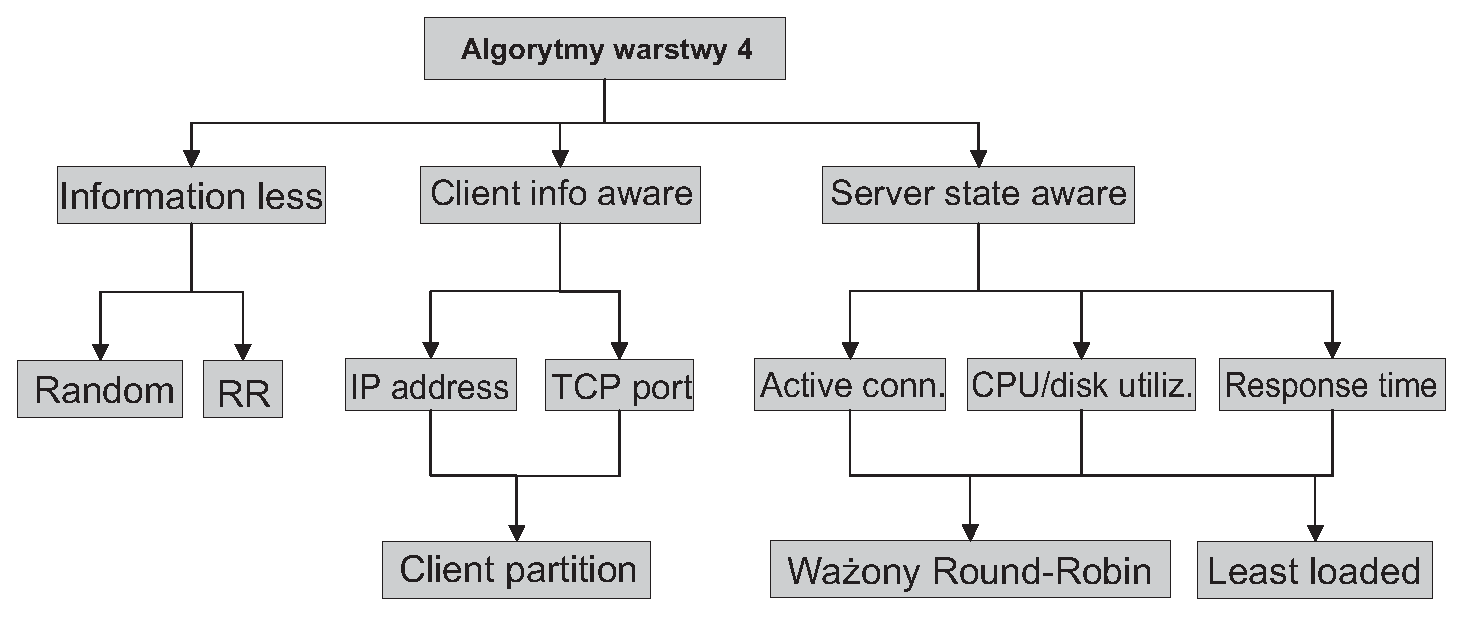
\includegraphics[width=4.9in]{./rysunki/level_4_alg.eps}
\caption{Algorytmy stosowane w dystrybutorach.}
\label{level_4_alg}
\end{figure}

Opr�cz informacji o tym, kto przesy�a zapytania do systemu webowego, mo�na r�wnie� uzyska� dane na temat pracy poszczeg�lnych 
serwer�w w systemie. Aby poprawi� jako�� szeregowania zapyta�, w algorytmie dokonuj�cym wyboru najlepszego serwera stosuje si� 
r�nego rodzaju metryki okre�laj�ce aktualne obci��enie serwer�w. Najcz�ciej stosowanymi algorytmami w tym przypadku s� Least 
loaded server oraz Weighted Round--robin. 
\begin{itemize}
\item W przypadku algorytmu Least loaded server dzi�ki wybranemu kryterium (okre�lonej metryce) wiemy, kt�ry z serwer�w 
powinien przyj�� kolejne zapytanie. Odbywa si� to na zasadzie: najmniej obci��ony serwer przyjmuje kolejne zlecenie. 
\item Stosuj�c algorytm Weighted Round--robin, przy wyborze kolejnego serwera mo�na uwzgl�dnia� metryk� jako parametr funkcji 
wyboru najlepszego serwera.

Wa�nym wi�c elementem funkcjonowania tego rozwi�zania jest dob�r metryki b�d�cej powy�szym parametrem. Istnieje 
mo�liwo�� kontrolowania nast�puj�cych parametr�w:
\begin{itemize}
\item input metric -- informacja pozyskiwana jest przez dystrybutor bez wsp�prcy z serwerami, np. liczba aktywnych po��cze� 
miedzy dystrybutorem a poszczeg�lnymi serwerami,
\item server metric -- informacja pozyskiwana jest przez serwery i dostarczana dystrybutorowi, np. wykorzystanie procesora lub 
dysku, czas miedzy otrzymaniem zapytania a wys�aniem odpowiedzi,
\item forward metric -- informacja pozyskiwana jest bezpo�rednio przez dystrybutor, np. emulacja zapyta� do serwer�w webowych.
\end{itemize}
\end{itemize}

\subsection{Algorytmy szeregowania wykorzystywane w prze��cznikach webowych}
Prze��czniki webowe maj� r�wnie� mo�liwo�� kontrolowania 100\% ruchu do serwer�w. Zatem i tu konieczne jest wykorzystanie jak 
najprostszych mechanizm�w zarz�dzania. W przypadku prostych rozwi�za� wystarczaj�co wydajne s� algorytmy statyczne. Sytuacja 
taka wyst�puje, gdy czasy realizacji zlece� przez serwery WWW s� bardzo zbli�one do siebie i nie wychodz� poza okre�lony 
przedzia� warto�ci.

W przypadku gdy w systemie wyst�puj� wi�cej ni� dwa ograniczenia czasu obs�ugi zlecenia, nale�y stosowa� algorytmy dynamiczne 
wykorzystuj�ce informacje o kliencie lub stanie serwera (client info or server state aware). Maj�c do dyspozycji 
heterogeniczne �rodowisko serwer�w trudno jest wybra� najlepszy, wsp�lny dla wszystkich parametr okre�laj�cy metryk� 
obci��enia serwera. W takim przypadku preferowane s� algorytmy wykorzystuj�ce informacje pochodz�ce od klient�w.
\begin{figure}[h]
\centering
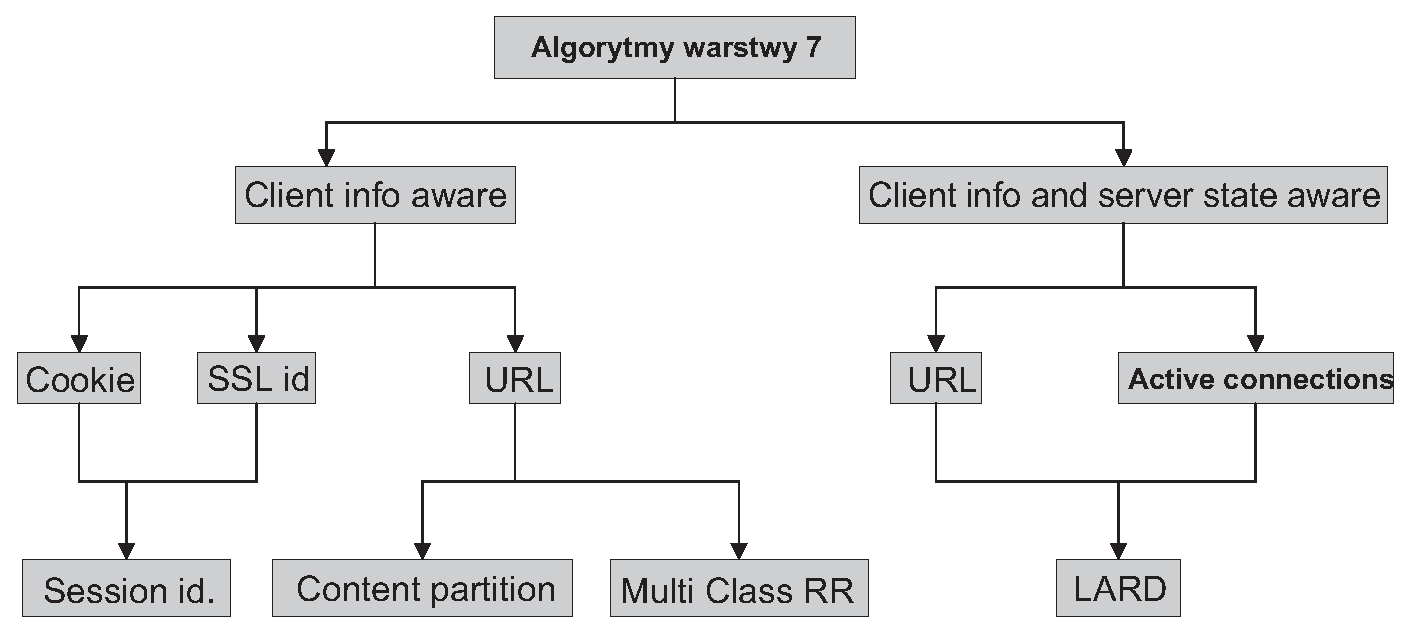
\includegraphics[width=4.9in]{./rysunki/level_7_alg.eps}
\caption{Algorytmy stosowane w prze��cznikach webowych.}
\label{level_7_alg}
\end{figure}

Jak wynika z rysunku \ref{level_7_alg}, istniej� trzy rodzaje algorytm�w opartych na informacjach o kliencie:
\begin{itemize}
\item Session identifiers -- odwo�ania HTTP, maj�ce ten sam identyfikator SSL lub ten sam znacznik cookie przypisywane s� do 
tego samego serwera -- zmniejsza to czas konieczny na ponown� identyfikacj� klienta,
\item Content partition -- podzia� zasob�w serwer�w mo�e nast�pi� ze wzgl�du na:
\begin{itemize}
\item typy plik�w -- dane, pliki graficzne, pliki audio umieszczone s� na specjalizowanych serwerach,
\item wielko�� plik�w -- du�e pliki na szybszych serwerach lub r�wnomierne roz�o�enie plik�w w przypadku serwer�w 
homogenicznych, 
\end{itemize}
\item Multi--class round--robin -- zasoby s� podzielone ze wzgl�du na z�o�ono�� obliczeniow� i czasow�, jaka zostanie 
wygenerowana podczas ich obs�ugi, np. po��czenia szyfrowane wymagaj� mocy obliczeniowej procesora, odwo�ania do bazy danych 
wymagaj� zwi�kszonej obs�ugi dysk�w, czy wreszcie pobieranie du�ych plik�w w znacznym stopniu obci��a sie�.
\end{itemize}

Zasada dzia�ania algorytmu wykorzystuj�cego informacje o kliencie i serwerze jest nast�puj�ca. Pierwsze zapytanie klienta o 
zasoby przekierowywane jest wed�ug algorytmu Least loaded server (metryk� jest ilo�� aktywnych po��cze� z serwerem). Pozosta�e 
zapytania klienta o ten sam zas�b przekierowywane s� do tego samego serwera. Dzi�ki temu zwi�kszona jest skuteczno�� odwo�a� 
do pami�ci podr�cznej (cache) tego serwera. Algorytm ten zwany jest Locality-Aware Request Distribution (LARD).

\subsection{Algorytmy szeregowania wykorzystywane w przypadku przekierowa� na poziomie protoko�u HTTP}

Gdy stosuje si� rozwi�zania oparte na warstwowej strukturze, istnieje mo�liwo�� zarz�dzania zapytaniami z poziomu protoko�u \cite{modele18}. 
Takie rozwi�zanie jest przezroczyste dla u�ytkownik�w. G��wnym celem stosowania tego mechanizmu jest zapobieganie 
przeci��eniom serwer�w webowych. Przekierowywanie odbywa si� poprzez przes�anie klientowi informacji w nag��wku: HTTP OK. 
302 -- Moved temporary to a new location.

Adres nowej lokalizacji mo�e by� podany w postaci nazwy domenowej lub adresu IP. Podanie adresu IP jest bardziej efektywne, 
poniewa� nast�puje bezpo�rednie odwo�anie do nowego serwera (klastra), a nie do serwera DNS.
Przekierowania mo�na realizowa� w zale�no�ci od kilku parametr�w \cite{modele13}. Proces przekierowa� mo�e dotyczy�:
\begin{itemize}
\item wszystkich stron,
\item tylko stron przekraczaj�cych okre�lon� wielko��,
\item tylko stron, kt�rych ilo�� obiekt�w sk�adowych przekracza okre�lon� liczb�,
\end{itemize}

Wyb�r serwera, kt�ry powinien przej�� zapytanie, mo�e odbywa� si� z wykorzystaniem jednej z poni�szych strategii:
\begin{itemize}
\item Round--robin,
\item Least Loaded,
\item Hash function,
\item Client to server proximity.
\end{itemize}

\section{Metody r�wnowa�enia obci��e� -- przyk�ady}

\subsubsection{R�wnowa�enie obci��e� z wykorzystaniem filtra datagram�w}

Inn� implementacj� rozproszonego algorytmu wsp�dzielenia obci��e� jest zastosowanie na ka�dym serwerze 
wchodz�cym w sk�ad klastra tzw. filtra datagram�w. Klaster taki powinien by� po��czony z Internetem poprzez 
pojedynczy router brzegowy. Ka�dy serwer w klastrze posiada skonfigurowane dwa adresy IP: adres ,,prywatny'' i 
jednakowy dla wszystkich serwer�w adres IP klastra. Router po otrzymaniu datagramu opatrzonego adresem IP 
klastra nadaje mu fizyczny (sprz�towy np. adres Ethernet) adres typu broadcast (je�eli do routera przy��czone 
s� tylko serwery nale��ce do klastra) lub multicast (je�eli klaster jest tylko wyr�nion� grup� w�r�d 
wszystkich host�w przy��czonych do serwera). Zastosowanie takiego adresu sprawia, �e karty sieciowe wszystkich 
serwer�w w klastrze akceptuj� datagram. Pomi�dzy sterownikiem karty sieciowej, a oprogramowaniem TCP/IP na 
ka�dym serwerze musi pracowa� specjalny proces, kt�ry zadecyduje, czy pakiet nale�y odrzuci� czy obs�u�y�. 
Proces ten nazywamy filtrem pakiet�w \cite{barylo34}. Decyzja o odrzuceniu lub obs�u�eniu datagramu podejmowana jest na 
podstawie zawarto�ci dw�ch struktur danych: tablicy po��cze� TCP (datagramy nale��ce do jednego po��czenia 
TCP musz� by� obs�ugiwane przez serwer kt�ry nawi�za� dane po��czenie) oraz tablicy zawieraj�cych wielko�� 
obci��enia poszczeg�lnych serwer�w klastra. Tablica ta jest uaktualniana przez same serwery. Ka�dy serwer musi 
wysy�a� okresowo komunikat typu broadcast zawieraj�cy wielko�� jego obci��enia. Je�eli do klastra nadchodzi 
datagram otwieraj�cy nowe po��czenie TCP (nag��wek TCP zawiera flag� SYN) serwer o najni�szym indeksie 
obci��enia w tablicy (indeksem tym jest zwykle liczba otwartych po��cze� TCP) jest zobowi�zany do jego 
przyj�cia. Dla zwi�kszenia wydajno�ci klastra w serwerach stosowa� mo�na dwie karty sieciowe: jedn� ze 
skonfigurowanym adresem IP klastra i drug� z prywatnym adresem serwera.  W takim przypadku pakiety, kt�re nie 
musz� by� filtrowane (np. wymiana danych SNMP) przechodzi� b�d� przez  ,,prywatn�'' kart�. Ten typ r�wnowa�enia 
dotyczy� mo�e ka�dej us�ugi korzystaj�cej z TCP, w szczeg�lno�ci WWW.
Pierwsz� komercyjn� implementacj� tego rozwi�zania by� pakiet oprogramowania Convoy Cluster firmy 
Valence Research przeznaczony dla systemu Microsoft Windows NT. Jako miar� obci��enia serwera przyj�to w nim 
ilo�� otwartych po��cze� TCP, a komunikaty og�aszaj�ce stan obci��enia wysy�ane by�y przez serwery co sekund�. 
Oprogramowanie umo�liwia�o dynamiczn� konfiguracj� klastra przez dodawanie lub usuwanie serwera z klastra bez 
przerywania pracy klastra. Serwery w klastrze musia�y powiela� swoje dane. W pierwszej wersji wymagane by�o 
stosowanie dw�ch kart sieciowych na ka�dym serwerze, a nadchodz�ce datagramy rozg�aszane by�y w trybie broadcast 
(dociera�y do ka�dego hosta w sieci lokalnej klastra, nawet je�li nie by� on serwerem) Wersja 2.0 Convoy 
Cluster wyeliminowa�a te niedogodno�ci i oferowa�a liczne dodatkowe mo�liwo�ci konfiguracyjne np. opcjonalne 
stosowanie pokrewie�stwa z klientem (ang. \emph{client affinity}), co umo�liwia obs�ug� wszystkich datagram�w 
nadchodz�cych od raz zidentyfikowanego (w trakcie nawi�zywania pierwszego po��czenia) klienta przez jeden 
serwer. W roku 1999 firma Microsoft wykupi�a od Valence Research technologi� Convoy Cluster i po 
,,kosmetycznych'' zmianach udost�pni�a j� w pakiecie Microsoft Windows NT 4.0 Enterprise Server pod nazw� 
Microsoft Load Balancing Service.
Najwa�niejsz� zalet� stosowania filtra pakiet�w jest jego du�a wydajno�� w por�wnaniu do 
scentralizowanych urz�dze� rozdzielaj�cych zadania (np. LSNAT). Uzyskiwane jest to dzi�ki temu, �e na �adnym 
etapie obs�ugi zadania nie s� modyfikowane datagramy i nie istnieje pojedynczy punkt podejmowania decyzji o 
obs�udze zadania. Wa�na jest r�wnie� �atwo�� konfiguracji klastra i du�a niezawodno�� (serwer, kt�ry ulega 
awarii przestaje wysy�a� komunikaty o stanie swego obci��enia, nie jest wi�c uwzgl�dniany w tablicach obci��enia 
serwer�w w pozosta�ych w�z�ach klastra i w ten spos�b nie bierze udzia�u w r�wnowa�eniu obci��e�). Koszt jaki 
nale�y ponie��, aby uzyska� te niew�tpliwie po��dane cechy to trudniejsza konfiguracja poszczeg�lnych serwer�w 
(konieczno�� instalacji i konfiguracji filtra pakiet�w) oraz du�y ruch w sieci lokalnej klastra wynikaj�cy z 
aktualizacji tablic obci��enia. Aktualizacje te musz� by� cz�ste, gdy� �atwo mo�na wyobrazi� sobie sytuacj�, w 
kt�rej serwer o najni�szym indeksie obci��enia ulega awarii. W takiej sytuacji pozosta�e serwery a� do 
aktualizacji swoich tablic obci��enia b�d� odrzuca� wszystkie datagramy otwieraj�ce nowe po��czenia, co z 
pewno�ci� nie jest zjawiskiem po��danym.

\subsubsection{R�wnowa�enie obci��e� z wykorzystaniem redirekcji HTTP}

Redirekcja jest  mechanizmem protoko�u HTTP, kt�ry zaprojektowano z my�l� o obs�udze sytuacji w kt�rych 
zas�b (plik) wskazywany przez pewien URL zmienia swoje fizyczne po�o�enie (zostaje przeniesiony na inny serwer) 
i w zwi�zku z tym uzyskuje inny URL. Aby nie zmusza� u�ytkownika do poszukiwania tego zasobu na w�asn� r�k� 
serwer WWW przechowuje tzw. tablice redirekcji. Jest to tablica zawieraj�ca URL, kt�re wcze�niej dotyczy�y 
zasob�w danego serwera, lecz obecnie zasoby te znajduj� si� pod innym URL. Tablica zawiera r�wnie� aktualny URL 
dla ka�dego przeniesionego zasobu. W przypadku zapytania o taki ,,zdezaktualizowany'' URL serwer WWW zwraca 
odpowied� HTTP typu ,,przeniesiono'' i jako dane przekazuje aktualny URL zasobu. Przegl�darka po otrzymaniu takiej 
odpowiedzi musi zestawi� nowe po��czenie z serwerem wskazanym przez otrzymany URL.

Opisany mechanizm w prosty spos�b wykorzysta� mo�na do pewnego rodzaju r�wnowa�enia obci��e� serwer�w 
WWW \cite{barylo22,barylo23}. W klastrze serwer�w wydzieli� mo�na tzw. serwer redirekcji, kt�rego nazwa DNS reprezentowa� 
b�dzie ca�y klaster. Jedynym zadaniem takiego serwera jest utrzymywanie tablicy redirekcji i przekierowanie 
nadchodz�cych zapyta� do odpowiedniego serwera z klastra. W takiej architekturze serwery zwykle nie powielaj� 
swych zasob�w, ka�dy z nich przechowuje cz�� danych udost�pnianych przez klaster, a to kt�ry z nich obs�u�y 
zapytanie determinowane jest przez rodzaj ��danych informacji. Przyk�adowo je�li pod nazw� www.pogoda.com 
dost�pny jest serwis prezentuj�cy prognoz� pogody dla ka�dego kontynentu to zasoby serwisu podzieli� mo�na 
pomi�dzy siedem serwer�w (po jednym dla ka�dego kontynentu) a pod adresem IP stanowi�cym odwzorowanie nazwy 
serwisu nale�y umie�ci� serwer redirekcji. W odpowiedzi na zapytanie o dowolny URL zaczynaj�cy si� np. od ci�gu 
www.pogoda.com/Azja/ serwer redirekcji dokonywa�by przekierowania do serwera przechowuj�cego dokumenty o 
pogodzie w Azji (np. wwwazja.pogoda.com) \cite{barylo22}. Poni�szy rysunek przedstawia schemat nawi�zywania 
po��czenia w przypadku stosowania redirekcji HTTP:
\begin{figure}[h]
\centering
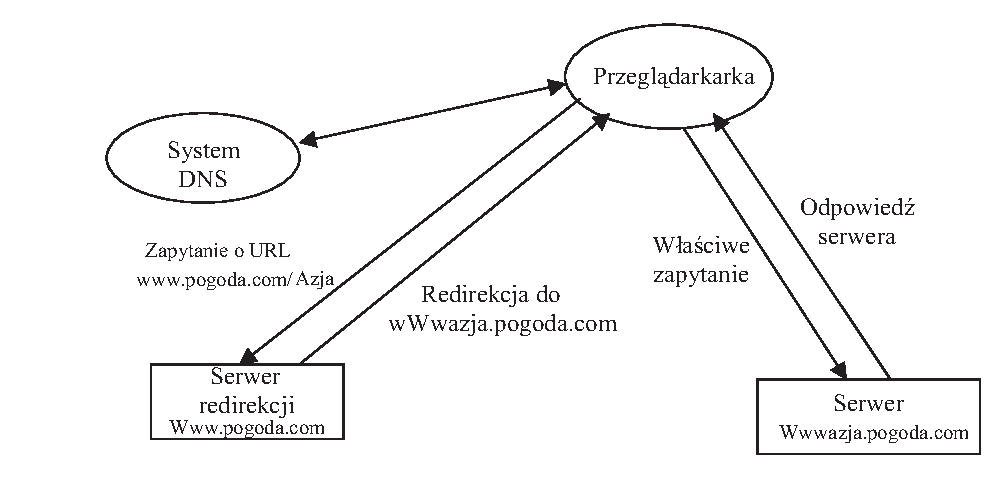
\includegraphics[width=4.9in]{./rysunki/redirekcja.eps}
\caption{Schemat redirekcji HTTP.}
\label{redirekcja}
\end{figure}

Stosowanie redirekcji ma zasadniczo dwie zalety. Po pierwsze utrzymanie statycznej tablicy redirekcji jest 
bardzo proste i tanie w implementacji, nie wymaga stosowania specjalnego sprz�tu ani oprogramowania. Po drugie, 
poniewa� u�ywane s� adresy URL, klaster stanowi�cy logiczn� ca�o�� mo�e by� rozproszony geograficznie tzn. 
serwer prezentuj�cy dane o pogodzie w Azji mo�e rzeczywi�cie znajdowa� si� na terenie tego kontynentu, co mo�e 
by� dobrym pomys�em przy za�o�eniu, �e o pogod� w Azji pyta� b�d� g��wnie Azjaci.
Redirekcja ma jednak wiele wad \cite{barylo30}. Przede wszystkim ograniczona jest do protoko�u HTTP, a jak wiadomo 
wiele ��cz hipertekstowych dokonuje prze��czenia do np. serwer�w FTP, kt�re cz�sto pracuj� na fizycznie tych 
samych komputerach, co serwery WWW. Druga wada jest wyra�nie widoczna na Rys. \ref{redirekcja}. Aby rozpocz�� pobieranie 
��danego dokumentu przegl�darka musi dokona� dw�ch po��cze�, najpierw z serwerem redirekcji, a nast�pnie z 
w�a�ciwym serwerem. Wprowadza to znaczne op�nienie i powoduje dodatkowe obci��enie sieci, kt�ra jest cz�sto 
w�skim gard�em wydajno�ci WWW. 

Prezentowane powy�ej podej�cie jest z gruntu statyczne i zak�ada wiedz� o tym, kt�re dane b�d� 
poszukiwane najcz�ciej, co umo�liwia aprioryczne przydzielenie najsilniejszego serwera w klastrze do obs�ugi 
najpopularniejszej cz�ci serwisu WWW. Poniewa� tablica redirekcji nie zawiera �adnych danych o obci��eniu 
poszczeg�lnych serwer�w trudno jest  dynamicznie uwzgl�dnia� takie dane podczas wyboru serwera. W literaturze 
proponowano architektury pi�trowe. Przyk�adowo dane dotycz�ce pogody w Azji mog�yby by� powielane pomi�dzy 
kilka serwer�w, kt�re raportowa�yby stopie� swego obci��enia, a na podstawie tych danych serwer redirekcji 
m�g�by dynamicznie aktualizowa� tablice redirekcji. Zbyt cz�sta aktualizacja tej tablicy czyni j� jednak 
bezu�yteczn� (tablica jest niedost�pna w trakcie aktualizacji), a zbyt rzadka powoduje nier�wnomierno�� 
obci��enia. Innym rozwi�zaniem jest zachowanie podzia�u na serwery tematyczne z mo�liwo�ci� dynamicznego 
przeniesienia cz�ci zawarto�ci z serwera mocno obci��onego na serwer posiadaj�cy rezerw� wydajno�ci. 
Aktualizacje tablicy redirekcji by�yby wtedy rzadsze, lecz procedura taka wymaga�aby kosztownego �ledzenia, 
kt�re pliki pobierane s� najcz�ciej (tylko przeniesienie takich plik�w znacz�co mo�e zmniejszy� obci��enie 
serwera), dodatkowo dane by�yby niedost�pne przez czas przenoszenia. Obydwie metody dynamicznego wykorzystania 
tablicy redirekcji mog� by� omini�te przez u�ytkownika, je�li po po��czeniu z serwerem docelowym umie�ci on 
zak�adk� (ang. \emph{bookmark}) na pobieranych stronach WWW. 
Statyczna redirekcja HTTP jest skuteczna tylko w przypadku serwis�w charakteryzuj�cych si� �atwym do 
przewidzenia wzorcem dost�pu do dokument�w.

\subsubsection{R�wnowa�enie obci��e� z wykorzystaniem NAT}

Mechanizm translacji adres�w sieciowych NAT (ang. \emph{Network Address Translation}) zosta� zaprojektowany z 
my�l� o mo�liwo�ci w��czenia prywatnych sieci lokalnych do Internetu z wykorzystaniem jednego, globalnie 
unikalnego adresu IP dla ca�ej sieci. W standardowej konfiguracji urz�dzeniem realizuj�cym NAT jest router 
brzegowy o adresie IP reprezentuj�cym ca�� sie�, kt�ry stanowi jedyne po��czenie pomi�dzy sieci� prywatn� a 
rozleg��. Hosty w sieci prywatnej nie musz� posiada� globalnie unikalnych adres�w IP, gdy� podczas nawi�zywania 
po��czenia z komputerem spoza sieci prywatnej urz�dzenie NAT zamienia adres nadawcy datagramu IP (pochodz�cy z 
sieci prywatnej) na sw�j w�asny, dokonuje przeliczenia odpowiednich sum kontrolnych i aby poprawnie kierowa� 
datagramami nale��cymi do jednego po��czenia TCP zapami�tuje w wewn�trznych tablicach parametry po��czenia 
(adresy i porty �r�d�owe i docelowe). Celem wprowadzenia mechanizmu NAT by�o zapewnienie pewnego stopnia 
bezpiecze�stwa sieciom prywatnym, gdy� je�li wewn�trz takiej sieci komputery nie posiadaj� globalnie unikalnych 
adres�w IP, to nie istnieje mo�liwo��  nawi�zania po��czenia z takim komputerem spoza sieci prywatnej. 
Istnieje wiele rozwi�za� komercyjnych realizuj�cych r�wnowa�enie (wsp�dzielenie)  obci��e� serwer�w 
WWW poprzez mechanizm NAT. Idea polega na kierowaniu zapyta� nadchodz�cych do klastra serwer�w poprzez 
specjalizowane urz�dzenie NAT, okre�lane czasem jako LSNAT (ang. \emph{Load Sharing NAT}), kt�re kierowa�oby zapytanie 
do konkretnego serwera \cite{barylo7}. Algorytm wed�ug kt�rego zapytanie by�yby kierowane do serwer�w mo�e uwzgl�dnia� 
r�nice w ich wydajno�ci jak i stopie� ich obci��enia, istnieje r�wnie� mo�liwo�� uwzgl�dnienia w nim numeru 
portu TCP, co sprawia, �e LSNAT stosowa� mo�na do r�wnowa�enia obci��e� wszystkich us�ug TCP. Obci��enie 
serwer�w okre�lane jest zazwyczaj na podstawie tablicy otwartych po��cze� utrzymywanej przez LSNAT dla ka�dego 
serwera. Aby dane te by�y aktualne konieczna jest analiza nag��wk�w TCP w celu wykrywania datagram�w 
zamykaj�cych po��czenie. Serwery w klastrze powinny powiela� swoje dane, gdy� wykorzystanie rozproszonego 
systemu plik�w powoduje zbyt du�e obci��enie sieci lokalnej klastra. Poni�ej schematycznie przedstawiono dwie 
typowe konfiguracje urz�dzenia NAT jako modu�u realizuj�cego  r�wnowa�enie obci��e�. Na ka�dym rysunku klaster 
serwer�w reprezentowany jest przez adres IP 172.87.0.100.

W takiej konfiguracji w datagramach przychodz�cych do klastra nast�puje zmiana adresu docelowego z adresu 
urz�dzenia LSNAT na adres wybranego serwera oraz zmiana adresu nadawcy na adres urz�dzenia LSNAT. W datagramach 
wysy�anych w przeciwnym kierunku adres nadawcy zmienia si� z adresu serwera na adres LSNAT a adres docelowy z 
adresu LSNAT na adres rzeczywistego odbiorcy datagramu. Takie post�powanie powoduje, �e wszystkie datagramy 
kierowane do klastra i z powrotem musz� przej�� przez urz�dzenie LSNAT, co umo�liwia skonfigurowanie klastra 
rozproszonego geograficznie. Dzieje si� tak kosztem utrzymywania w LSNAT bardziej rozbudowanej (w stosunku do 
poprzedniej konfiguracji) tablicy po��cze�, kt�ra umo�liwia�aby identyfikacj� ka�dego po��czenia. Identyfikacji 
tej dokonuje si� wykorzystuj�c numery port�w TCP (wraz z translacj� adres�w datagramu dokonuje si� zmiany 
numeru portu �r�d�owego na unikaln� dla danego serwera warto�� powy�ej 5000, identyfikacji odpowiedzi adresata
dokonuje si� na podstawie adresu serwera, kt�ry j� wys�a� i numeru portu docelowego). Powy�sza konfiguracja 
pracowa� mo�e r�wnie� z adresami prywatnymi, uniemo�liwia to jednak u�ycie serwer�w odleg�ych geograficznie.
Poni�ej przedstawiono kr�tki opis dw�ch popularnych rozwi�za� komercyjnych wykorzystuj�cych mechanizm 
NAT do r�wnowa�enia obci��e� serwer�w WWW.

Rozwi�zania korzystaj�ce z mechanizmu NAT do r�wnowa�enia obci��e� s� znacznym post�pem w stosunku do metod 
opisanych wcze�niej w tej pacy. Umo�liwiaj� skuteczne uwzgl�dnienie stopnia obci��enia poszczeg�lnych serwer�w 
w klastrze jak i ich indywidualnych w�a�ciwo�ci. LSNAT umo�liwia rozr�nianie po��cze� na podstawie numer�w 
port�w TCP jak i r�wnowa�enie obci��e� pomi�dzy serwery odleg�e geograficznie. Metoda ta nie jest jednak 
pozbawiona wad. W oczywisty spos�b urz�dzenie LSNAT staje si� w�skim gard�em wydajno�ci klastra, gdy� ca�y 
ruch pomi�dzy klasterem, a Internetem musi przez nie przechodzi�. Je�li wzi�� pod uwag�, �e w przypadku WWW 
obj�to�� odpowiedzi serwera jest co najmniej dziesi�ciokrotnie wi�ksza ni� zapytanie, jasnym staje si�, �e w 
obliczu ci�g�ego wzrostu liczby u�ytkownik�w, najwydajniejsze nawet urz�dzenie LSNAT mo�e w ko�cu ograniczy� 
wydajno�� klastra. Nale�y r�wnie� zauwa�y�, �e zmiana adresu IP w nag��wku datagramu poci�ga za sob� 
konieczno�� wyliczenia nowej sumy kontrolnej dla ca�ego datagramu. Jest to operacja czasoch�onna przez co 
wprowadza op�nienie w transmisji danych jak i konieczno�� kolejkowania pakiet�w w samym urz�dzeniu (trudno 
oczekiwa�, �e nawet urz�dzenie przetwarzaj�ce klika pakiet�w r�wnolegle poradzi sobie bez op�nie� z ca�ym 
przechodz�cym przez nie ruchem). Ta w�a�ciwo�� LSNAT znacznie ogranicza jego skalowalno��, gdy� dodawanie 
nowych serwer�w do klastra w prosty spos�b zwi�ksza kolejk� pakiet�w w urz�dzeniu, a� do momentu, w kt�rym 
przekroczone zostan� jego mo�liwo�ci lub cierpliwo�� u�ytkownik�w. 

\subsubsection{R�wnowa�enie obci��e� poprzez ,,p�--po��czeniowe'' marszrutowanie TCP}

Rozpatruj�c przedstawione kolejno w tej pracy metody r�wnowa�enia obci��e� mo�na zauwa�y� pewn� 
prawid�owo��. Ot� im dana metoda jest bardziej skuteczna i zaawansowana koncepcyjnie, tym w ni�szej warstwie 
sieciowej operuje. Redirekcja HTTP i RR--DNS dzia�a�y powy�ej warstwy transportowej, w og�le nie ingeruj�c w 
zawarto�� datagram�w IP. Rozwi�zania oparte o LSNAT i DPR pracowa�y w warstwie sieciowej i aby skutecznie 
rozdziela� zadania pomi�dzy serwery musia�y dokonywa� modyfikacji (adres�w i sum kontrolnych) w nag��wkach  
datagram�w IP. Metoda opisana w tym punkcie operuje w warstwie fizycznej  i do rozdzia�u zada� nie musi 
zmienia� zawarto�ci datagram�w IP.

,,P�--po��czeniowe'' marszrutowanie TCP (ang. \emph{half--connection TCP routing}) jest opatentowan� przez 
firm� IBM technologi�, kt�ra leg�a u podstaw zasady dzia�ania pakietu oprogramowania Network Dispatcher \cite{barylo35,barylo36}. 
W swej podstawowej konfiguracji pakiet ten umo�liwia zestawienie klastra z�o�onego z po��czonych 
sieci� lokaln� serwer�w korzystaj�cych TCP lub UDP (w szczeg�lno�ci serwer�w WWW) i udost�pnienie go pod 
jednym adresem IP. W klastrze tym serwery maj� unikalne globalnie lub lokalnie adresy IP i  musz� powiela� 
swoje dane. W obszarze tej samej sieci lokalnej, w kt�rej dzia�a klaster, musi by� wyznaczony komputer, na 
kt�rym pracowa� b�dzie oprogramowanie Network Dispatcher. Komputer ten musi posiada� dwa adresy IP, jeden z 
nich, tzw. adres NFA (ang. \emph{Non--Forwarding Address}) jest ,,osobistym'' adresem komputera, pod kt�rym mo�na 
skontaktowa� si� z pracuj�cym na tym komputerze oprogramowaniem (np. z agentem SNMP). Drugi adres, to adres 
reprezentuj�cy klaster serwer�w, wszystkie datagramy IP opatrzone tym adresem b�d� przetwarzane przez program 
Network Dispatcher i na podstawie algorytmu wsp�dzielenia obci��e� przekazywane do jednego z serwer�w w 
klastrze. Dispatcher zmienia jedynie docelowy adres fizyczny (sprz�towy) datagramu, zawarty w nag��wku 
sprz�towym, dodawanym przed nag��wek IP (np. w nag��wku Ethernet). Dzi�ki temu datagramy wysy�ane przez serwer 
w odpowiedzi mog� by� kierowane bezpo�rednio do klienta, bez konieczno�ci ponownego przej�cia przez 
oprogramowanie Network Dispatcher (w celu np. przywr�cenia oryginalnych adres�w IP). St�d pochodzi nazwa tej 
metody -- ,,p�--po��czeniowe'' marszrutowanie TCP. Serwer wysy�aj�c odpowied� dokonuje standardowej zamiany adres�w 
IP nadawcy i odbiorcy pobieraj�c obydwa te adresy z nag��wka otrzymanego datagramu. Jak pami�tamy adresem 
docelowym jest w tym datagramie adres klastra (komputera, na kt�rym pracuje Dispatcher), wi�c adres ten stanie 
si� adresem nadawcy odpowiedzi, co sprawi, �e kolejne datagramy dotycz�ce danego po��czenia skierowane zostan� 
na adres Network Dispatcher--a \cite{barylo36}.

Adres IP ka�dego serwera w klastrze jest r�ny od adresu klastra. Fakt, �e pomimo to oprogramowanie 
TCP/IP w serwerze akceptuje pakiety opatrzone adresem klastra jest mo�liwy dzi�ki dodaniu aliasu do adresu 
interfejsu p�tli zwrotnej (ang. \emph{loopback interface}) w ka�dym serwerze. Do standardowego adresu 127.0.0.1 
dodawany jest jako alias adres klastra (w przypadku przedstawionym na rysunku 139.37.38.39). Mo�liwo�� 
nadawania wielu adres�w interfejsowi p�tli zwrotnej jest jedynym wymaganiem Dipatcher-a w stosunku do serwer�w.
Poniewa� Network Dispatcher rozr�nia porty TCP i UDP mo�liwe jest r�wnowa�enie obci��e� powodowanych 
przez dowolny protok� korzystaj�cy z TCP lub UDP m.in. HTTP (WWW), FTP, SSL, SMTP, POP3 czy Telnet. Poniewa� 
wszystkie serwery powielaj� swoje dane, mo�liwa jest sytuacja w kt�rej np. plik HTML opisuj�cy stron� WWW 
pobierany jest z serwera A, a pliki graficzne sk�adaj�ce si� na stron� pobierane s� z serwera B.
W celu zarz�dzania po��czeniami Network Dispatcher przechowuje dwie struktury danych- tablic� po��cze� 
aktywnych (otwartych) i tablic� nowo przydzielonych po��cze�. Tablica otwartych po��cze� s�u�y do poprawnego 
kierowania datagram�w dotycz�cych nawi�zanego po��czenia TCP (po��czenie TCP nie mo�e by� przez Dipatcher 
przekazane pomi�dzy serwerami). Zawiera ono adres IP nadawcy i numer �r�d�owego portu TCP oraz adres IP serwera, 
kt�ry obs�uguje po��czenie i numer portu docelowego TCP oraz pole stanu po��czenia. Pozycje z tej tablicy s� 
usuwane po wykryciu w nag��wku TCP flagi FIN lub RST. Ilo�� po��cze� otwartych na danym serwerze jest r�wnie� 
uwzgl�dniana podczas obliczenia wagi serwera. Tablica nowo przydzielonych po��cze� s�u�y do zapami�tania jak 
wiele po��cze� zosta�o przydzielonych do danego serwera od ostatniego od�wie�enia wag serwer�w i jako miara 
pr�dko�ci zmian obci��enia serwera wykorzystywana jest do obliczenia jego wagi.

Je�eli na adres Dispatcher--a przychodzi datagram nie nale��cy do �adnego z po��cze� zapisanych w 
tablicy aktywnych po��cze�, oznacza to, �e jest to nowe po��czenie i nale�y przydzieli� serwer do jego obs�ugi. 
Dispatcher utrzymuje cykliczn� list� serwer�w zawieraj�c� ich wagi. Waga serwera oddaje stopie� jego obci��enia 
i jest obliczana przez Dispatcher okresowo dla klastra (dla wszystkich serwer�w jednocze�nie). Dispatcher 
pami�ta numer i wag� serwera do kt�rego przydzielono ostatnie po��czenie TCP i rozpoczynaj�c przeszukiwanie 
listy od tego miejsca poszukuje serwera o wadze wi�kszej lub r�wnej zapami�tanej wadze (im wi�ksza waga, tym 
mniej obci��ony serwer). Do znalezionego w ten spos�b serwera przydzielane jest nowe po��czenie, co znajduje 
odwzorowanie w tablicy aktywnych po��cze�. 

Waga dla ka�dego serwera obliczana jest na podstawie ilo�ci otwartych po��cze� TCP, ilo�ci nowo 
przydzielonych po��cze�, stopnia obci��enia procesora w serwerze (miara ta uwzgl�dnia r�wnie� obci��enie 
wynikaj�ce z zada� uruchamianych lokalnie i pochodzi od modu�u ISS (ang. \emph{Interactive Session Support}) pakietu 
Network Dispatcher, ISS uwzgl�dnia r�wnie� indywidualne w�a�ciwo�ci serwera) oraz na podstawie danych 
pochodz�cych z tzw. Advisor--�w. Advisor jest programem symuluj�cym klienta danego protoko�u i bada jak szybko 
serwer jest w stanie zareagowa� na typowe dla danego protoko�u ��danie. Np. Advisor HTTP wysy�a do serwera 
��danie HTTP GET / (prze�lij domy�lny dokument g��wnego katalogu w serwisie) i jako wynik zwraca czas, po kt�rym 
otrzyma� pierwszy bajt odpowiedzi. Proporcje z jakimi poszczeg�lne elementy wchodz� w sk�ad wagi, jak i 
cz�stotliwo�� od�wie�ania wag ustalane s� przez administratora klastra.
Network Dispatcher posiada wiele cech wyr�niaj�cych go spo�r�d przedstawionych wcze�niej rozwi�za�. 
Jest oczywi�cie wolny od niekorzystnych cech RR--DNS i nie modyfikuje datagram�w IP, a analiza, kt�r� na nich 
prowadzi (zapami�tanie adres�w i port�w, wykrywanie flag), nie jest czasoch�onna. Dodatkowo ruch przechodz�cy 
przez Dispatcher--a stanowi� tylko datagramy nadchodz�ce do klastra (typowo mniejsze od odpowiedzi), dzi�ki 
czemu nie jest �atwo (w przeciwie�stwie do urz�dze� LSNAT) tak obci��y� Dispatcher--a by sta� si� ,,w�skim 
gard�em'' wydajno�ci klastra. W przeciwie�stwie do rozwi�zania z zastosowaniem DPR, Dispatcher nie wymaga 
specjalistycznego oprogramowania pracuj�cego na serwerze, wi�c nie obci��a go np. zadaniem przetwarzania 
datagram�w IP.

Pierwszy prototyp Network Dispatcher--a obs�ugiwa� Internetowy serwis IO w Atlancie w 1996. Kolejne, 
ju� komercyjne wersje obs�ugiwa�y takie wydarzenia jak turniej US Open i IO w Nagano w 1998 oraz mecze szachowe 
Deep Blue vs. Garri Kasparow. Szczytowe obci��enie klastra w przypadku IO w Nagano osi�gn�o 110 414 zapyta� na
 minut�, a mimo to r�wnowa�enie obci��e� przy u�yciu Network Dispatcher--a zapewni�o wszystkim u�ytkownikom dobry 
czas odpowiedzi i zadowalaj�cy transfer.

\subsubsection{R�wowa�enie obci��e� poprzez bezpo�rednie routowanie -- \emph{Direct Routing}}

Architektura ta jest podobna do wykorzystywanej w produkcie firmy IBM -- oprogramowaniu SecureWay Network Dispatcher. 

Adres wirtualny serwera jest wsp�dzielony poprzez poszczeg�lne nody i load balancer. Interfejs sieciowy dystrybutora jest 
skonfigurowany tak�e do wirtualnego adresu, kt�ry jest wykorzystywany do przyjmowania pakiet�w przychodz�cych oraz do 
bezpo�redniego routowania pakiet�w do wybranych serwer�w. Wszystkie rzeczywiste serwery maj� swoje non--arp aliasy interfejsu 
sieciowego skonfigurowane z adresem wirtualnym lub bezpo�rednio przekierowuj� pakiety przeznaczone na adres wirtualny do 
lokalnych gniazd, w ten spos�b, �e rzeczywiste serwery mog� przenosi� pakiety tylko lokalnie. Zar�wno load balancer jak i 
rzeczywiste serwery musz� mie� interfejsy sieciowe fizycznie skojarzone z HUB--em lub switchem. Wygl�da to w ten spos�b, �e
dystrybutor po prostu zmienia adres MAC na adres rzeczywistego serwera i retransmituje do niego pakiet. 

\section{Przyk�ady produkt�w stosowanych do r�wnowa�enia obci��enia wielokomputerowych serwer�w WWW}

\subsection{LinuxVirtualServer}

Linux Virtual Server jest wysoce skalowalnym i dost�pnym serwerem zbudowanym na klastrze rzeczywistych serwer�w wraz 
z mo�liwo�ci� realizacji r�wnowa�enia obci����. System ten oparty jest na systemie Linux. Architektura tego rozwi�zania
jest (jak i pozosta�e) przezroczysta dla klienta i odbywa si� na poziomie protoko�u IP (warstwa czwarta). 

Rzeczywiste serwery mog� by� po��czone w obr�bie sieci lokalnej lub geograficznie rozproszone w sieci WAN. Fron-endem tych
rzeczywistych serwer�w jest dystrybutor (load balancer), kt�ry marszrutuje ��dania do r�nych serwer�w oraz powoduje, �e
r�wnoleg�e us�ugi dzia�aj�ce w obr�bie klastra wydaj� si� by� jedn� wirtualn� us�ug� dla ca�ego klastra na jednym adresie IP.
Skalowalno�� w tym systemie oznacza, �e w przezroczysty spos�b mo�na dodawa� i usuwa� poszczeg�lne nody do klastra. Wysoka 
dost�pno�� jest realizowana poprzez detekcj� uszkodzonych nod�w lub niesprawnych demon�w oraz r�wnoczesn� rekonfiguracj�
systemu.

Virtual Server mo�na implementowa� na trzy sposoby:
\begin{description}
\item[Virtual Server poprzez NAT] -- zalet� tego rozwi�zania jest fakt, �e rzeczywiste serwery mog� pracowa� na dowolnym
systemie operacyjnym, kt�ry w�ada protoko�em TCP/IP. Rzeczywiste serwery maj� prywatny adresy IP i tylko one s� potrzebne
dystrybutorowi do pracy. Wad� tego rozwi�zania jest raczej niewielka skalowalno��, poniewa� w tym wypadku \emph{load balancer}
mo�e stanowi� w�skie gard�o ca�ego systemu gdy liczba pod��czonych serwer�w b�dzie wynosi� oko�o 20 lub wi�cej. Jest to
spowodowane tym, �e zar�wno ruch przychodz�cy (niewielki) jak i wychodz�cy (o wiele wi�kszy) s� przepisywane przez dystrybutora.
Mo�na to omin�c poprzez korzystanie z pozosta�ych rozwi�za� Virtual Servera lub poprzez rozwi�zanie hybrydowe z DNS i kilkoma
osobnymi Virtual Serverami;
\item[Virtual Server poprzez Tunelowanie IP] -- w tym wypadku load balancer tylko przekazuje
ruch wchodz�cy do poszczeg�lnych rzeczywistych serwer�w, za� one odpowiadaj� bezpo�rednio do u�ytkownik�w. W tym rozwi�zaniu 
jak wida� serwer virtualny mo�e si� sk�ada� i z ponad 100 serwer�w i nadal dystrybutor nie b�dzie stanowi� w�skiego gard�a.
Maksymalna wydajno�� Virtual Servera w tym przypadku mo�e si�ga� powy�ej 1Gbps -- w przypadku gdy dystrybutor dysponowa�
b�dzie 100Mbps kart� sieciow�. Rozwi�zanie oparte na tunelowaniu IP mo�e by� u�ywane do serwer�w wirtualnych w bardzo 
wysokich wydajno�ciach, szczeg�lnie dobrych do tworzenia virtualnych proxy serwer�w. Wad� tego rozwi�zania jest to, �e ka�dy
serwer musi umie� dokonywa� enkapsulacji IP (tunelowanie IP) wewn�trz IP; 
\item[Virtual Server poprzez bezpo�rednie routowanie]\footnote{ang. \emph{Direct Routing}} -- opisany powy�ej. Wad� tego 
rozwi�zanie jest brak mo�liwo�ci rozbudowy wirtualnego serwera powy�ej sieci lokalnej, jednak�e w por�wnaniu z poprzedni�
architektur� rzeczywiste serwery nie potrzebuj� pos�ugiwa� si� enkapsulacj� IP.
\end{description}

W po��czeniu z ka�d� implementacj� Virtual Server korzysta z nast�puj�cych algorytm�w dystrubuuj�cych pakiety:
\begin{itemize}
\item marszrutowanie algorytmem Round--Robin;
\item marszrutowanie algorytmem Weighted Round--Robin (statyczne wagi, bez wykorzystywania informacji o stanie system�w);
\item marszrutowanie typu Least Connection (dynamiczny algorytm -- opisany w tekscie);
\item marszrutowanie typu Weighted Least Connection (jak wy�ej + statycznie nadawane wagi poszczeg�lnym serwerom);
\item marszrutowanie Locality--Based Least Connection;
\item marszrutowanie Locality--Based Least Connection witch Replcation;
\item marszrutowanie typu Destination Hashing;
\item marszrutowanie typu Source Hashing.
\end{itemize}

Zalet� Virtual Servera jest jego dzia�anie w obr�bie j�dra co oznacza wysok� wydajno�� i stabilno��. Kolejn� zalet� jest 
dost�pno�� kodu �r�d�owego (oprogramowanie typu OpenSource) co oznacza mo�liwo�� modyfikacji kodu w zale�no�ci od potrzeb.

\subsection{Cisco LocalDirector}

LocalDirector jest nazw� rodziny urz�dze� produkowanych przez firm� Cisco. Urz�dzenia te s�u�� do 
r�wnowa�enia obci��e� dowolnych serwer�w wykorzystuj�cych TCP (np. serwery WWW, FTP, SSL) \cite{barylo30,barylo31}. 
LocalDirector instalowany jest w konfiguracji przedstawionej na Rys. \ref{LocalDirector} z wykorzystaniem adres�w prywatnych, 
\begin{figure}[h]
\centering
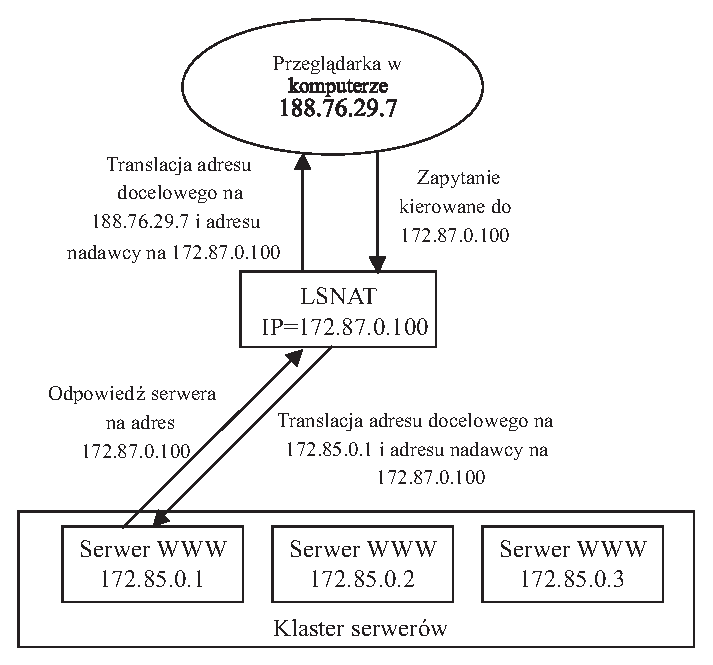
\includegraphics[width=4in]{./rysunki/LocalDirector.eps}
\caption{LSNAT symetrycznie zmieniaj�cy adres IP.}
\label{LocalDirector}
\end{figure}

musi wi�c by� instalowany jako jedyne po��czenie pomi�dzy klasterem a bramk� (ang. \emph{gateway}) do sieci rozleg�ej. 
LocalDirector wymaga powielania zawarto�ci pomi�dzy serwerami w klastrze. Serwery mog� by� po��czone z 
LocalDirector-em poprzez sie� Ethernet, FastEthernet lub FDDI. Wyb�r serwera dokonywany jest sekwencyjnie na 
podstawie wag uwzgl�dniaj�cych indywidualne w�a�ciwo�ci serwera i jego obci��enie w postaci liczby otwartych 
po��cze� TCP. LocalDirector sprawdza czy serwer si� nie za�ama� poprzez okresowe nawi�zywanie z nim po��czenia 
kontrolnego (Ping, HTTP GET /). Producent zapewnia, �e LocalDirector, w zale�no�ci od modelu, jest w stanie 
obs�u�y� od 7000 do 25000 po��cze� na sekund� przy przepustowo�ci od 80 Mbit/sek. do 400 Mbit/sek. Istnieje 
mo�liwo�� pi�trowej konfiguracji LocalDirector-a. Kilka rozproszonych geograficznie klaster�w, z kt�rych ka�dy 
obs�ugiwany jest przez jedno urz�dzenie LocalDirector, mo�na zaprezentowa� jako jeden klaster z u�yciem tzw. 
GlobalDirectora. GlobalDirector to w rzeczywisto�ci serwer DNS rozdzielaj�cy zapytania pomi�dzy klastery na 
zasadzie podobnej do RR--DNS. 

\subsection{F5 Labs BigIP}

BigIP firmy F5 Labs jest tzw. rozwi�zaniem ,,pod klucz'' (ang. \emph{turn--key solution}). Oznacza to, �e dostarczany 
jest tak jak urz�dzenie sprz�towe (np. LocalDirector), cho� w rzeczywisto�ci jest to komputer pracuj�cy pod 
kontrol� specjalizowanego oprogramowania i systemu operacyjnego firmy F5 Labs. BigIP umo�liwia r�wnowa�enie 
obci��e� ka�dego serwera korzystaj�cego z protoko�u TCP lub UDP \cite{barylo32,barylo33}. Urz�dzenie mo�e by� pod��czone w 
konfiguracji przedstawionej na Rys. \ref{LocalDirector} lub Rys. \ref{LocalDirector1} w obydwu jednak przypadkach, aby uniemo�liwi� omini�cie 
\begin{figure}[h]
\centering
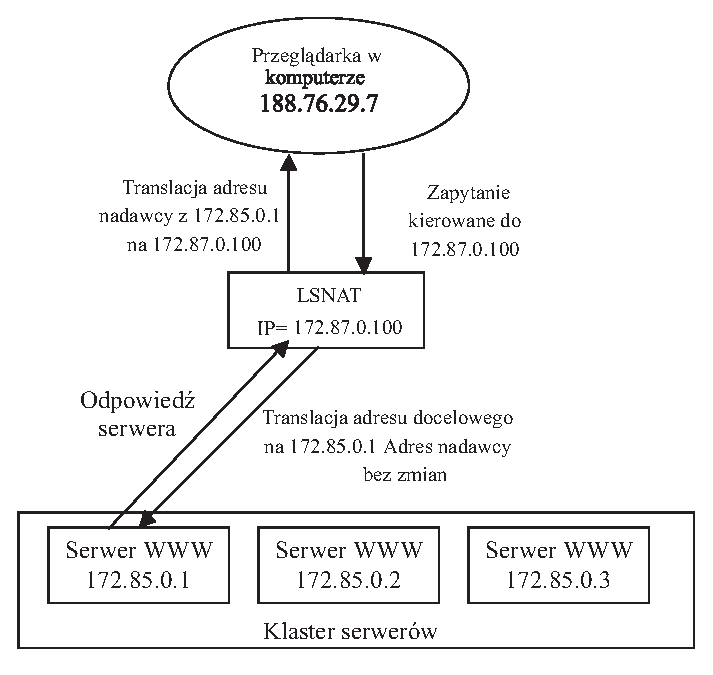
\includegraphics[width=4in]{./rysunki/LocalDirector1.eps}
\caption{LSNAT zmieniaj�cy jeden z adres�w IP}
\label{LocalDirector1}
\end{figure}

mechanizmu r�wnowa�enia obci��e�, BigIP powinien znajdowa� si� pomi�dzy klasterem serwer�w, a bramk� do 
Intetrnet-u. BigIP mo�na po��czy� z klasterem poprzez sie� Ethernet, FastEthernet, FDDI lub opcjonalnie 
GigaBitEthernet. Urz�dzenie oferuje do wyboru siedem algorytm�w rozdzia�u zada�. Trzy z nich to algorytmy 
statyczne, s� to: algorytm cykliczny (ang. \emph{Round--robin}); algorytm proporcjonalny przydzielaj�cy zadania wed�ug 
ustalonych na sta�e wag i algorytm priorytetowy, kt�ry umo�liwia wydzielenie w klastrze grup serwer�w o 
okre�lonym priorytecie i rozdzia� zada� do grup, w ka�dej z grup serwer do obs�ugi konkretnego zadania 
wskazywany jest cyklicznie. Pozosta�e algorytmy s� dynamiczne i uwzgl�dniaj� obci��enie poszczeg�lnych 
serwer�w. S� to algorytm LC (ang. \emph{Least Connections}) przydzielaj�cy zadania do serwera utrzymuj�cego najmniej 
otwartych po��cze�, algorytm wyznaczaj�cy ten serwer, kt�ry najszybciej odpowie na zapytanie kontrolne (np. 
HTTP GET /), tzw. algorytm obserwacyjny b�d�cy kombinacj� powy�szych i algorytm predyktywny, kt�ry przydziela 
zadania (po��czenia) do serwera, kt�rego obci��enie (mierzone jako kombinacja ilo�ci otwartych po��cze� i czasu 
odpowiedzi na zapytanie kontrolne) zmniejsza�o si� najszybciej w ci�gu np. ostatnich 5 sekund.
Konkretne modele BigIP wyposa�one s� w procesory Intel Pentium II 450 do 600 MHz pami�� RAM 128 MB do 
1GB i dysk twardy 4 GB do 8.4 GB. Producent gwarantuje przepustowo�� od 170 Mbit/sek. do 350 Mbit/sek. i 
obs�ug� do 20000 zapyta� na sekund�.
	
\subsection{IBM SecureWay Network Dispatcher}

W zwi�zku z tym, �e pakiet ten jest jednym z g��wnych element�w tej pracy, jego dok�adny opis i konfiguracja znajduje si� 
w nast�pnym rozdziale (Rozdz. \ref{r05}).


\chapter{System do zarz�dzania wielokomputerowym serwerem WWW}
\label{r05}

\section{Wst�p}
W tym rozdziale zostanie przedstawiony opis konfiguracji stanowiska u�ytego do bada� nad charakterystykami 
r�nych konfiguracji i algorytm�w klastra serwer�w WWW zestawionego w �rodowisku systemu AIX i Windows NT z 
wykorzystaniem pakietu IBM WebSphere Performance Pack. Opisana zostanie konfiguracja sieci komputerowej, w kt�rej zosta�y 
przeprowadzone badania oraz charakterystyka poszczeg�lnych test�w.

\section{Charakterystyka u�ytego oprogramowania}

\subsection{IBM WebSphere Performance Pack}

IBM WebSphere Performance Pack jest oprogramowaniem infrastrukturalnym WWW wi���cym ze sob� skalowalno��, niezawodno�� i 
wydajno��, kt�re to cechy s� niezb�dne dla aplikacji e-biznesu zar�wno w �rodowiskach lokalnych jak i rozproszonych. Jego 
funkcje ��cz� ze sob� znakomity caching, zarz�dzanie plikami i r�wnowa�enie obci��enia, kt�re razem kompensuj� wrodzone 
s�abo�ci Internetu by wspiera� krytyczne aplikacje biznesowe.

IBM WebSphere Performance Pack sk�ada si� z trzech g��wnych element�w, kt�re to pozwalaj� zredukowa� obci��enie serwera WWW, 
zwi�kszy� dyspozycyjno�� zasob�w (zawarto�ci) i zwi�kszy� wydajno�� serwera WWW \cite{GettingStarted}:
\begin{description}
\item[Wsp�dzielenie plik�w]\

Komponent zajmuj�cy si� wsp�dzieleniem plik�w, znany jako IBM AFS Enterprise File System (AFS), jest systemem plik�w 
pozwalaj�cym wsp�pracuj�cym hostom (klientom i serwerom) efektywnie wsp�dzieli� zasoby system�w plik�w poprzez 
zar�wno LAN jak i WAN. Prowadzi on replikacj� informacji pomi�dzy wieloma serwerami w czasie rzeczywistym, gwarantuj�c przy 
tym sp�jno�� danych, dost�pno��, stabilno�� i efektywno�� w administrowaniu, wymaganych przez du�e, rozproszone serwisy webowe.
\item[Keszowanie i filtrowanie]\

Komponent odpowiedzialny za pami�� podr�czn� i filtrowanie zawarto�ci webowej, znany jako IBM Web Traffic Express (WTE) jest 
proxy serwerem, kt�ry dostarcza wysoce skalowalnych funkcji keszowania i filtrowania zwi�zanych z przesy�aniem ��da� webowych 
i dostarczaniem adres�w URL. Modu� ten jest w stanie zredukowa� kosztown� szeroko�� wykorzystywanego pasma dost�powego i w 
szybszy spos�b, oraz z mniejszymi op�nieniami dostarcza� informacje do klienta.
\item[R�wnowa�nie obci��enia]\

Modu� odpowiedzialny za r�wnowa�enie obci��e�, znany jako IBM SecureWay Network Dispatcher jest serwerem zdolnym do 
dynamicznego monitorowania i r�wnowa�enia aplikacji i serwer�w TCP w czasie rzeczywistym. G��wn� zalet� tego komponentu jest 
mo�liwo�� dynamicznego zwi�zania ze sob� wielu serwer�w TCP tak, �e wygl�daj� z sieci jak pojedynczy logicznie serwer.
\end{description}

Ka�dy z element�w IBM WebSphere Performance Pack mo�e by� zainstalowany oddzialenie od pozosta�ych -- tak�e na innych 
komputerach. Dzi�ki zwi�zaniu tylu element�w w jednym pakiecie - klient otrzymuje oprogramowanie o scentralizowanej 
administracji i zminimalizowanym koszcie. 

Procedury instalacyjne pozwalaj� wybra�, kt�ry komponent nale�y zainstalowa� i na jakich maszynach w sieci maj� si� one 
znajdowa�. Oprogramowanie to jest portowane na nast�puj�ce platformy: AIX (od wersji 4.2.1), Solaris (od wersji 2.6) oraz 
MS Windows NT i 2000.

\subsection{Web Traffic Express}
WTE jest naraz kaszuj�cym serwerem proxy i filtrem zawarto�ci pakiet�w. Zaawansowane keszowanie pozwala zminimalizowa� 
wykorzystanie przepustowo�ci zwi�kszaj�c przy tym pewno��, �e klienci sp�dz� znacznie mniej czasu podczas pobrania tej samej 
informacji kilka razy \cite{WTEUsersGuide,WTEProgramming}. 

Tradycyjny proxy serwer przesy�a ��dania dla URL od klienta i podaje je dalej do serwera przeznaczenia. WTE daje co� wi�cej; 
pozwala zapisa� lub keszowa� dokumenty, kt�re przesy�a oraz serwowa� je podczas p�niejszych ��da� ze swojego keszu, a nie ze 
�r�d�owego serwera. Co oznacza, �e klient ��dany dokument otrzymuje szybciej przy zmniejszonym obci��eniu ��cz. 

Modu� ten posiada tak�e dodatkowe cechy takie jak:
\begin{itemize}
\item mo�liwo�� utrzymania bardzo du�ego keszu;
\item opcj� automatycznego od�wie�ania tej cz�ci pami�ci podr�cznej zawieraj�cej najcz�ciej popobierane strony;
\item mo�liwo�� keszowania tak�e tych stron, kt�rych nag��wek wymaga by by�y zawsze pobierane ze �r�d�owego serwera;
\item konfigurowania okresowego porz�dkowania keszu z informacji bezu�ytecznych w celu poprawy wydajno�ci i utrzymania 
efektywno�ci jego dzia�ania;
\item Remote Cache Access (RCA) - w�a�ciwo�� pozwalaj�ca na wielu maszynom z WTE uwsp�lniania tego samego keszu poprzez 
rozproszony system plik�w, taki jak AFS, w celu zredukowania redundancji zawarto�ci.
\end{itemize}

Dodatkowo WTE pozwala na ustawianie filtrowania zawarto�ci na poziomie serwera proxy -- pozwalaj�c na takie zabiegi jak np. 
blokowanie URL--�w. Zwielokrotnione serwery WTE mog� by� obci��eniowo zr�wnowa�one.

Kolejn� cech� jak� posiada ten modu� jest mo�liwo�� pracy jako przezroczysty proxy -- czyli taki, do kt�rego dzia�ania nie jest 
potrzebna �adna zmiana w konfiguracji przegl�darki klienta -- WTE pracuje wtedy na porcie serwera WWW. 

\subsection{IBM SecureWay Network Dispatcher}
Jest to jedno z pierwszych komercyjnych rozwi�za�, kt�re pozwala zwi�kszy� wydajno�� i zapewni� ci�g�� prac� serwis�w 
internetowych. Znalaz�o ono ju� szerokie zastosowanie w znacz�cych serwisach WWW, takich jak serwisy prowadzone w trakcie 
olimpiad w Atlancie i Nagano. 
System jest przeznaczony do obs�ugi serwer�w webowych zbudowanych w technologii klastrowej. Klaster jest grup� serwer�w 
webowych obs�uguj�cych jedn� witryn� WWW. Wszystkie serwery w klastrze posiadaj� t� sam� zawarto�� i zapytanie mo�e by� 
obs�u�one przez dowolny z nich serwer. Pojedyncze zapytanie obs�ugiwane jest przez jeden z aktualnie sprawnych serwer�w. 
IBM SecureWay Network Dispatcher sk�ada si� z trzech komponent�w: podsystemu Dispatcher, podsystemu Interactive Session 
Support (ISS) oraz podsystemu Content--based Routing (CBR). Komponenty te mog� by� u�ywane ��cznie lub ka�dy z 
osobna \cite{LoadBalancingWithND}.

\subsubsection{Komponent Dispatcher}

Podstawowym komponentem systemu jest Dispatcher, kt�rego zadaniem jest zapewnienie r�wnomiernej dystrybucji zapyta� 
realizowanych za po�rednictwem protoko�u TCP/IP mi�dzy wieloma serwerami realizuj�cymi t� sam� us�ug� w konfiguracji 
klastrowej. Funkcjonowanie Network Dispatcher'a opiera si� na architekturze przedstawionego wcze�niej dystrybutora. 
Dispatcher mo�e r�wnowa�y� obci��enia w obr�bie sieci lokalnej lub rozleg�ej. Dla ka�dego klastra definiuje si� porty, kt�re 
chcemy, aby by�y obs�ugiwane przez klaster, nast�pnie serwery, kt�re b�d� dostarcza� us�ugi na ka�dym z zdefiniowanych port�w. 
Dispatcher mo�e obs�ugiwa� wiele klastr�w \cite{NDUsersGuide}. 

Wysok� dost�pno�� serwisu osi�gni�to poprzez dzia�anie samego Dispatcher'a, kt�ry wykrywa niesprawne serwery w klastrze i 
omija je przy dystrybucji zapyta� oraz poprzez wprowadzenie drugiego systemu Dispatcher'a. W podstawowym trybie pracy 
Dispatcher wymaga, aby wszystkie serwery w klastrze by�y w tej samej podsieci co Dispatcher. W�wczas, aby podwy�szy� 
dost�pno�� serwisu, mo�emy skonfigurowa� drugi system Dispatcher'a, kt�ry pe�ni� b�dzie rol� maszyny zapasowej i czuwaj�cej w 
gotowo�ci do przej�cia zadania r�wnowa�enia obci��enia w przypadku, gdyby maszyna podstawowa Dispatcher'a przesta�a dzia�a� 
poprawnie. Mechanizm typu heartbeat zapewnia monitorowanie stan�w przez obie maszyny, podstawow� i zapasow� oraz przej�cie 
zada� w przypadku wyst�pienia awarii.
\begin{figure}[h]
\centering
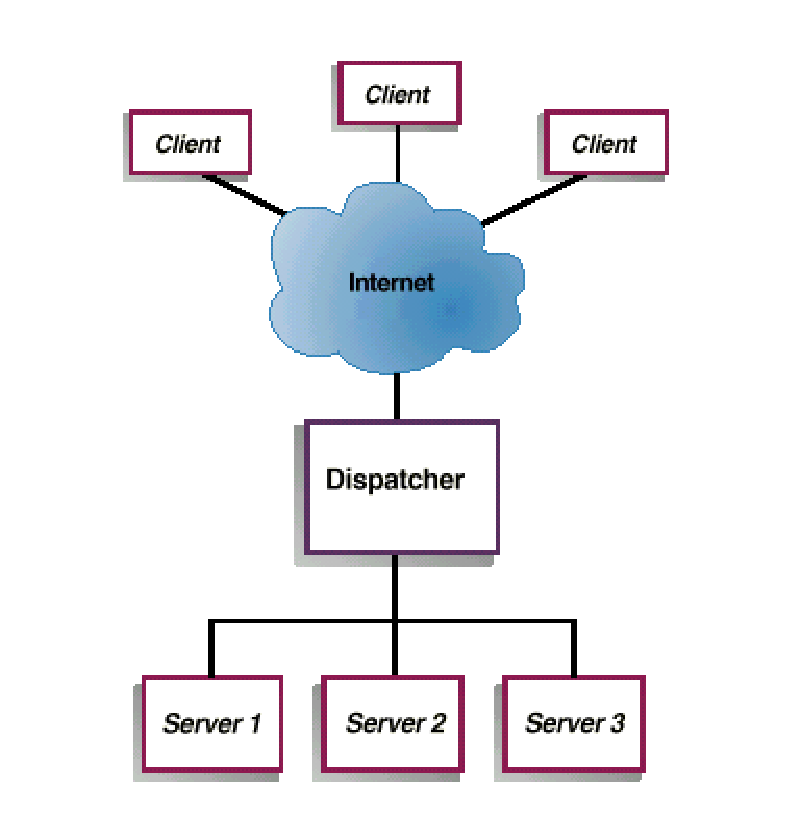
\includegraphics[width=3in]{./rysunki/dispatcher.eps}
\caption{Konfiguracja logiczna modu�u dispatcher}
\label{dispatcher}
\end{figure}

Dispatcher realizuje swoje zadania za pomoc� trzech wewn�trznych komponent�w: Egzekutora, Menad�era i Doradc�w. Egzekutor 
realizuje r�wnowa�enie obci��e�. Dla pakietu wysy�anego w ramach nowego po��czenia mi�dzy klientem a serwerem WEB Dispatcher 
sprawdza, kt�ry z serwer�w mo�e przej�� obs�ug� zlecenia na ��danym przez klienta porcie i adresie klastra. Nast�pnie, dla 
ka�dego takiego serwera, na podstawie zgromadzonych wag okre�laj�cych poziom obci��e� serwer�w, okre�la serwer najmniej 
obci��ony, do kt�rego przekazuje pakiet. Je�li po��czenie ju� istnieje, wtedy bez �adnego przetwarzania pakiet jest natychmiast
wysy�any do tego samego serwera, kt�ry zosta� wybrany podczas inicjalizacji po��czenia. Rozdzia� zlece� mi�dzy serwery bazuje 
na warto�ciach wag wskazuj�cych na mo�liwo�� potencjalnego obci��enia serwera -- np. je�eli jeden serwer ma wag� 2, a drugi ma 
wag� 1, to serwer o wadze 2 powinien dosta� dwa razy wi�cej ��da� ni� ten o wadze 1. Wagi mog� by� ustawiane r�cznie lub przez 
Menad�era. Najcz�ciej do ustawiania wag korzysta si� z Menad�era, kt�ry ustawia wagi automatycznie i w spos�b adaptacyjny, z 
uwzgl�dnieniem aktualnych warunk�w pracy klastra. Menad�er mo�e korzysta� z wewn�trznych licznik�w systemowych oraz z 
informacji dostarczanych przez inne komponenty systemu, takich jak ISS czy WLM. Zarz�dca decyduje kt�ry z serwer�w jest 
najmniej obci��onym poprzez obserwacj� wag serwer�w, kt�re to okresowo analizuje i uaktualnia. Decyzj� jak� serwerowi nada� 
wag� podejmuje opieraj�c si� na czterech parametrach:
\begin{itemize}
\item liczba aktywnych po��cze� realizowanych na ka�dym serwerze TCP;
\item liczba nowych po��cze� na ka�dym serwerze TCP;
\item danych wej�ciowych pochodz�cych od doradc�w;
\item informacji pochodz�cych od narz�dzi monitoruj�cych prac� systemu, takich jak ISS;
\end{itemize}

U�ywanie zarz�dcy jest opcjonalne, ale je�li 
nie jest on u�ywany, r�wnowa�enie obci��enia jest dokonywane przy u�yciu marszrutowania algorytmem wa�onego Round Robina, 
gdzie wagi poszczeg�lnych serwer�w WWW s� nadawane statycznie; 

Aby da� administratorowi wi�ksz� kontrol� nad tym, gdzie kierowane b�d� ��dania r�nego typu pochodz�ce od r�nych grup 
u�ytkownik�w, wprowadzono poj�cie regu� i grup serwer�w im podleg�ych, tj. serwer�w, w�r�d kt�rych b�dzie realizowane 
r�wnowa�enie obci��enia w razie spe�nienia regu�y. Dla Dispatcher'a dost�pne s� regu�y bazuj�ce na: adresie IP klienta, porcie 
klienta, porze dnia, po��czeniach na sekund� dla danego portu, aktywnych po��czeniach dla danego portu. Regu�y daj� mo�liwo�� 
implementacji wysokiej jako�ci us�ug dla wybranych klient�w b�d� w okre�lonej porze dnia. Dost�pna jest tak�e regu�a ,,zawsze 
prawdziwe'', kt�ra oznacza spe�nienie zadanego warunku dla wszystkich przyjmowanych zlece�.
\begin{figure}[h]
\centering
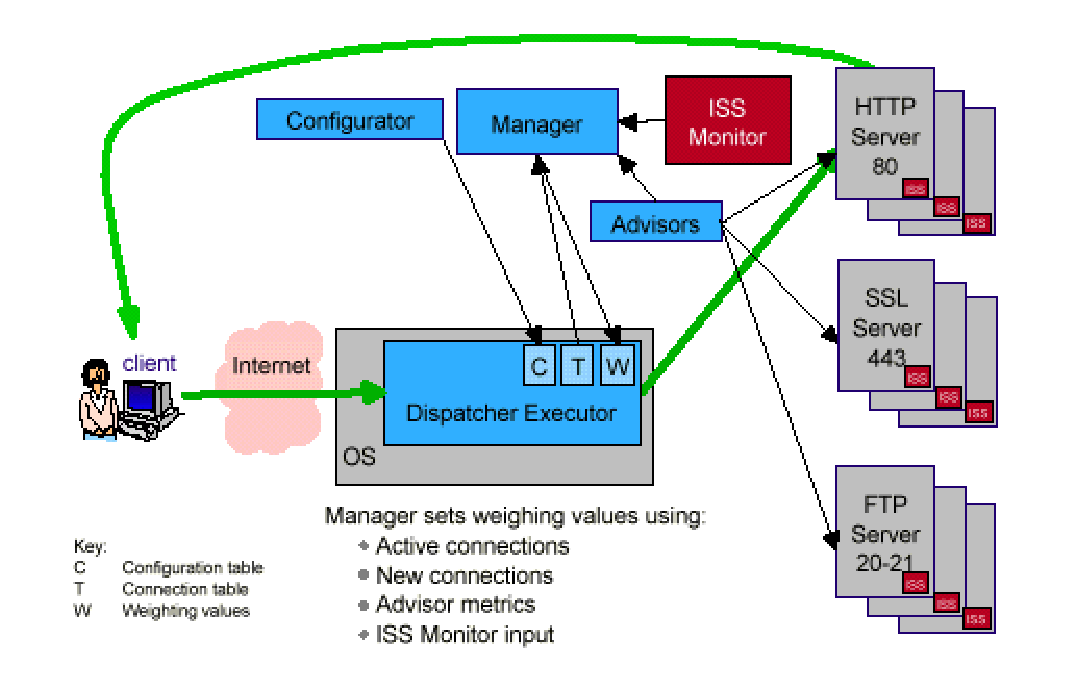
\includegraphics[width=5in]{./rysunki/executor.eps}
\caption{Architektura Network Dispatcher-a}
\label{dispatcher1}
\end{figure}

Zadaniem doradc�w jest zbieranie informacji na temat obci��enia serwer�w. Doradcy sprawdzaj� r�wnie�, czy serwery, na kt�rych 
dokonywane jest r�wnowa�enie obci��e�, funkcjonuj� prawid�owo. Doradcy okresowo otwieraj� po��czenia TCP i wysy�aj� do serwera 
wiadomo�� z ��daniem specyficznym dla danego typu doradcy. Po wys�aniu wiadomo�ci Doradcy czekaj� na odpowied�. Po jej 
otrzymaniu wi�kszo�� Doradc�w szacuje warto�� obci��enia serwera na podstawie czasu, jaki up�yn�� nim serwer zwr�ci� odpowied� 
na ��danie i zg�aszaj� ten czas (w milisekundach) Menad�erowi, aby ten na podstawie tej i innych informacji oszacowa� warto�� 
wag poszczeg�lnych serwer�w. 

Wraz z produktem IBM SecureWay Network Dispatcher dostarczeni s� doradcy: HTTP, FTP, Telnet, NNTP, POP3, SMTP, SSL, WTE, TCP, 
Ping, WLM. Istnieje r�wnie� mo�liwo�� napisania w�asnego doradcy. 

\subsubsection{Komponent Interactive Session Support}

Interactive Session Support (ISS) jest komponentem wsp�pracuj�cym z Domain Name Server (DNS) w jednym z trzech mo�liwych 
tryb�w pracy: DNS--Update, DNS--Replace lub DNS--Ignore. Komponent ten mo�e by� r�wnie� wykorzystany do zbierania informacji na 
temat obci��enia serwer�w, kt�r� nast�pnie przekazuje do Dispatcher'a. W trybie DNS--Update ISS uaktualnia serwer nazw DNS. W 
tym trybie dzia�a on w po��czeniu z serwerem nazw w celu mapowania nazw DNS na adresy IP serwer�w najlepiej nadaj�cych si� do 
obs�ugi danego zadania. W trybie DNS--Replace ISS spe�nia dla ograniczonej podgrupy sieci funkcj� serwera nazw, nie zawiera 
jednak wszystkich funkcji standardowego DNS. W trybie DNS--Ignore, ISS dzia�a w po��czeniu z Dispatcher'em w celu lepszego 
r�wnowa�enia obci��e�.
\begin{figure}[h]
\centering
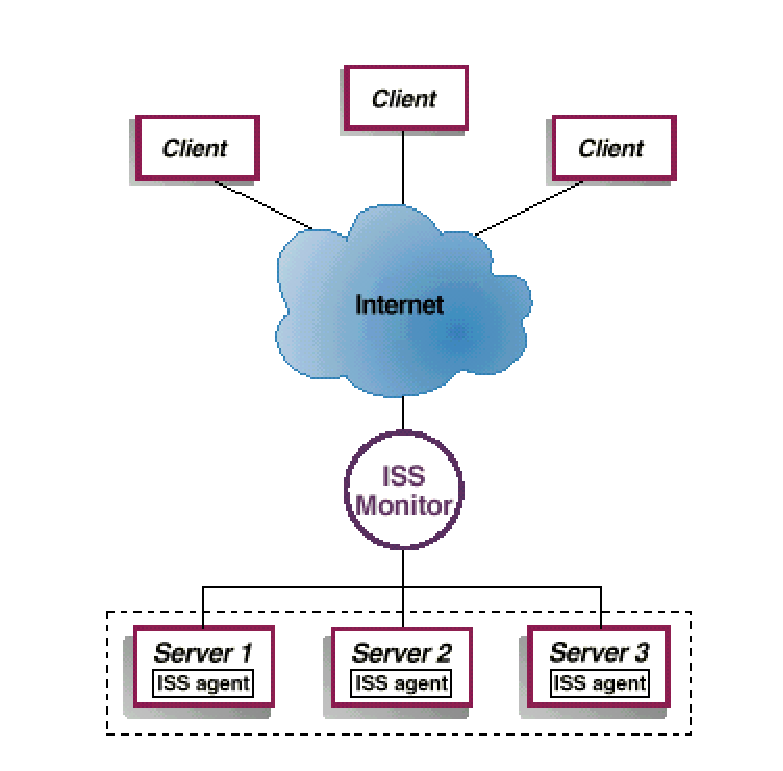
\includegraphics[width=3in]{./rysunki/ISS.eps}
\caption{Konfiguracja logiczna modu�u Interactive Session Support}
\label{ISS}
\end{figure}

Obci��enie na poszczeg�lnych w�z�ach mo�e by� okre�lane poprzez pomiar wykorzystania r�nych zasob�w, takich jak ilo�� wolnej 
pami�ci, u�ycie procesora czy licznik proces�w. ISS pos�uguje si� jedn� z trzech strategii alokacji zlece�: RoundRobin, Best, 
i Statistical RoundRobin.

Przy u�yciu algorytmu RoundRobin, ISS r�wnowa�y obci��enia serwer�w w spos�b klasyczny dla tej strategii. Z danej grupy 
serwer�w ISS wybiera na okre�lony przedzia� czasu jeden serwer, kt�ry b�dzie obci��any w tym przedziale czasu. ISS nie zwraca 
w�wczas uwagi na poziom obci��enia serwera, ale te� nie zaleci serwera, kt�ry niedomaga. Takie podej�cie mo�e funkcjonowa� 
dobrze, pod warunkiem �e obci��enie wywo�ywane przez klient�w jest r�wnomierne. Zalet� tej metody jest brak obci��enia 
serwer�w poprzez procesy pomiarowe. Natomiast jej du�� wad� jest brak elastyczno�ci. Metoda ta mo�e powodowa�, �e np. serwer, 
kt�ry ju� jest bardzo obci��ony, mo�e by� dalej preferowany przez ISS, gdy� nie sko�czy� si� jeszcze przydzielony mu czas.
Stosuj�c strategi� Best, w czasie trwania okre�lonego interwa�u, ISS trasuje ��dania do serwera, kt�ry na pocz�tku tego 
interwa�u mia� najni�szy poziom obci��enia. Tak jak w przypadku poprzedniej metody, korzystaj�cy z niej ISS nie zaleci 
serwera, kt�ry przesta� funkcjonowa�. Ta metoda selekcji sprawdza si� bardzo dobrze dla ka�dego czasu trwania po��cze�, pod 
warunkiem, �e cz�sto�� nowych po��cze� b�dzie relatywnie niska w stosunku do ustawionego interwa�u czasu przydzia�u dla 
pojedynczego serwera. Ta strategia jest przyjmowana domy�lnie przez system.
W strategii Statistical RoundRobin, ISS r�wnowa�y obci��enia na podstawie statystyk obci��enia, kt�re generuje dla wszystkich 
serwer�w. Wykorzystuje te statystyki do budowy profilu najbardziej i najmniej obci��onych serwer�w, a nast�pnie w ci�gu 
trwania interwa�u ,,heartbeat'' rozdziela ��dania pomi�dzy serwery, proporcjonalnie do ich obci��enia. R�wnie� przy u�yciu tej 
metody ISS nie zaleci niedomagaj�cego serwera. Metoda ta sprawdza si� wsz�dzie tam, gdzie wyst�puje du�a cz�sto�� 
kr�tkotrwa�ych po��cze�.

\subsubsection{Komponent Content Base Routing}
 
Komponent CBR mo�e by� skonfigurowany z WTE (Web Traffic Express) dla serwer�w HTTP, lub jako CBR proxy (bez wsp�pracy z WTE)
dla serwer�w IMAP i POP3. CBR wsp�pracuje wesp� z Web Traffic Express, w ten spos�b, �e klient wysy�a ��danie do WTE, kt�ry 
jest skonfigurowany by m�c korzysta� z CBR; CBR musi by� zainstalowany na tej samej maszynie co serwer WTE. WTE wypytuje 
komponent CBR kt�ry serwer ma obs�u�y� ��danie. Gdy CBR otrzyma ��danie pr�buje je dopasowa� do ustawionych regu�. Je�li 
pasuj�, CBR wybiera serwer, z grupy skonfigurowanych do odbierania konkretnego typu ��da�, jednocze�nie r�wnowa��c pomi�dzy 
t� grup� serwer�w obci��enie. 

CBR jest bardzo podobny w strukturze do pakietu Dispatcher. Trzy kluczowe elementy CBR (Egzekutor, Menad�er i Doradcy) 
wsp�pracuj� by zr�wnowa�y� i rozdzieli� przychodz�ce ��dania pomi�dzy serwery w zbli�ony spos�b jak w Dispatcherze. 
Jednak�e w przeciwie�stwie do modu�u Dispatcher -- CBR nie oferuje funkcji zwi�kszonej dost�pno�ci. Jednak�e mo�na po��czy� 
kilka serwer�w CBR i r�wnowa�y� ich obci��enie poprzez serwer ND, kt�ry to mo�e sprawdza� czy �aden z CBR serwer�w nie 
przesta� odpowiada�.

\begin{itemize}
\item CBR z WTE (obs�uguj�cy ruch HTTP)

Komponent CBR wsp�pracuj�c z Web Traffic Express dzia�a jako proxy serwer przekierowuj�c rz�dania klient�w do odpowiednich
serwer�w. Modu� WTE jest proxy serwerem, pozwalaj�cym manipulowa� pami�ci� podr�czn� w celu szybkiego transferu dokument�w
przy niewielkich wymaganiach dotycz�cych przepustowo�ci sieci. CBR za� jest w stanie przefiltrowa� zawarto�� stron WWW 
korzystaj�c ze specyficznych ci�g�w warunk�w nazywanych rolami. CBR daje mo�liwo�� okre�lenia grupy serwer�w, kt�re powinny
przej�� ��danie opieraj�c si� na wyra�eniach regularnych pasuj�cych do zawarto�ci ��dania. Poniewa� CBR pozwala na
,,przywi�zanie'' poszczeg�lnych serwer�w do ka�dego typu ��dania nast�puje zr�wnowa�enie obci��enia serwer�w. CBR potrafi
tak�e wykrywa� kiedy serwer przestaje odpowiada� wy��czaj�c routing ��da� do niego. Zastosowane w module CBR algorytmy
r�wnowa�enia obci��enia s� identyczny z tymi zastosowanymi w komponencie Dispatcher. 

Spos�b dzia�ania CBR: gdy klienckie ��danie jest przesy�ane do WTE proxy nast�puje tu korelowanie zawarto�ci ��dania
z regu�ami zdefiniowanymi w module CBR. Je�li zbi�r regu� pasuje do zawarto�ci ��dania jeden z serwer�w ,,zwi�zanych'' z 
obs�ug� tego typu ��da� zostaje wybrany do przyj�cia ��dania. Wtedy WTE jako proxy serwer przekierowuje do wybranego serwera 
��danie. Jak wida� modu� WTE musi by� uruchomiony zanim CBR zostanie skonfigurowany, poniewa� dzia�a on jako podproces WTE.
Oczywi�cie oba modu�y musz� znajdowa� si� na tej samej maszynie.

Oznacza to podzia� farmy serwer�w na cz�ci realizuj�ce odpowiedni typ ��da�. Taki podzia� jest przezroczysty dla klienta. 
Mo�na np. podzieli� witryn� na dwie cz�ci -- kilka serwer�w realizuj�cych tylko ��dania CGI, a pozosta�e reszt� ruchu HTTP.
Pozwala to na realizacj� intensywnie przetwarzanych skrypt�w CGI w spos�b nie koliduj�cy z prac� reszty serwer�w WWW 
obs�uguj�cych normalny ruch HTTP -- co oznacza dla klienta lepszy og�lny czas odpowiedzi. W ten spos�b komputery o wi�kszej
mocy obliczeniowej mo�na przeznaczy� na obs�uge normalnego ruchu bez kosztownego upgradu wszystkich komputer�w.
\begin{figure}[h]
\centering
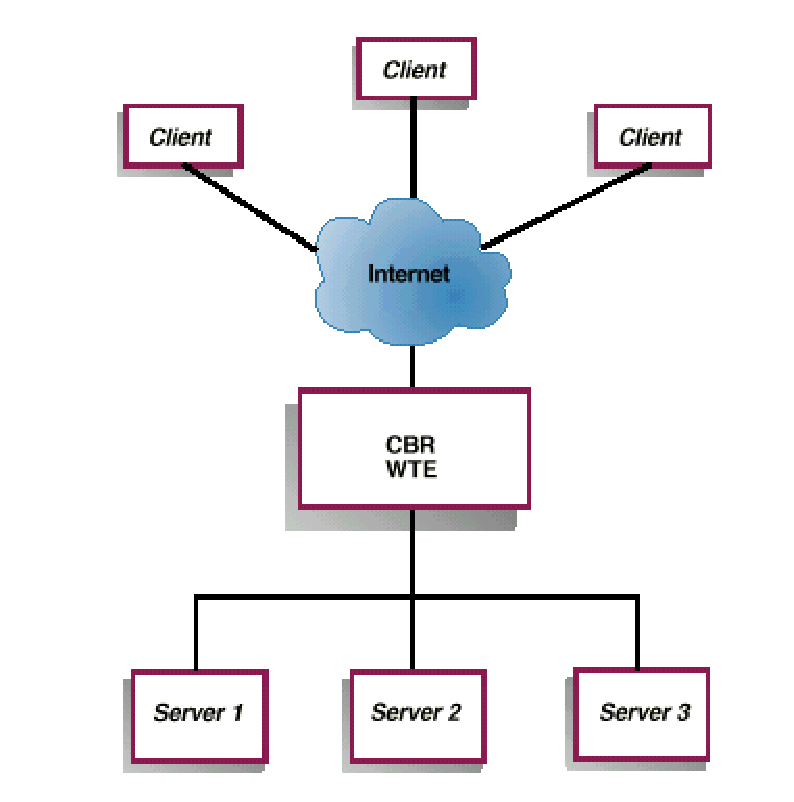
\includegraphics[width=3in]{./rysunki/CBR-WTE.eps}
\caption{Konfiguracja logiczna modu�u Content Base Routing (wraz z WTE)}
\label{CBR}
\end{figure}


Inn� mo�liwo�ci� podzia�u serwera WWW jest bezpo�rednie przekierowanie klient�w, kt�rzy chc� dosta� si� do stron wymagaj�cych
rejestracji, do jednego typu serwer�w, a reszt� do pozosta�ych. Wtedy obs�ug� stron wymagaj�cych rejestracji zajmuj� si�
np. komputery o wi�kszej mocy obliczeniowej i klienci, kt�rzy s� ju� zarejestrowani maj� lepszy czas odpowiedzi ni� inni. 

Wybieraj�c role dokonuj�ce r�wnowa�enia obci��enia nale�y sprawdzi� czy wszystkie ��dania do klastra WWW posiadaj� role, 
na podstawie ktorych mo�na wybra� serwer. Je�li tak nie jest, tzn. je�li przychodz�ce ��danie nie pasuje do �adnej roli, klient
otrzyma komunikat o b��dzie pochodz�cy z WTE. Najprostszym rozwi�zaniem jest stworzenie roli zawsze prawdziwej z bardzo 
wysokim priorytetem i ,,przywi�zanie'' jej do osobnej grupy serwer�w.

\item CBR proxy (obs�uguj�cy ruch IMAP i POP3)

CBR bez WTE mo�e by� proxy wybieraj�cym odpowiedni serwer opieraj�c si� na ID u�ytkownika i ha�le. Nie wspiera wtedy opartego
na rolach r�wnowa�enia obci��e�.
\end{itemize}

\subsection{Content Base Routing -- konfiguracja}

CBR mo�e zosta� skonfigurowany jako proxy dla us�ug opartych o protoko�y POP3 lub IMAP -- dzia�a wtedy bez wsp�pracy
z modu�em WTE, lub tez jako narz�dzie r�wnowa��ce obci��enie ruchu HTTP -- systemem proxy jest wtedy WTE  \cite{NDUsersGuide}.

Modu� ten mo�na skonfigurowa� za pomoc� linii komend lub z pomoc� graficznego interfejsu u�ytkownika
(\emph{GUI}). Modu� Content Base Routing jest bardzo podobny w architekturze do Dispatchera. Sk�ada si� on z trzech
funkcjonalnych cz�ci:
    \begin{itemize}
    \item Egzekutor -- zajmuje si� r�wnowa�eniem obci��enia zapyta� klienckich. Jest zawsze uruchomiany je�li CBR
    jest w u�yciu;
    \item Menad�er -- ustala wagi dla poszczeg�lnych serwer�w opieraj�c si� na:
        \begin{itemize}
        \item wewn�trznych licznikach Egzekutora;
        \item informacjach zbieranych z serwer�w przez doradc�w;
        \item informacjach z program�w monitoruj�cych prace systemu, takich jak ISS czy WLM.
        \end{itemize}
        Korzystanie z menad�era jest opcjonalne. Jednak�e gdy jest on nieu�ywany -- r�wnowa�enie obci��enia jest
        realizowane za pomoc� algorytmu statycznego Wa�onego Round--Robin opartego na domy�lnych wagach, a
        doradcy nie b�d� wtedy dost�pni.
    \item Doradcy -- wypytuj� serwery oraz analizuj� dane o ich stanie, by nast�pnie z tak spreparowanych danych
    Menad�er ustali� odpowiednie wagi. Korzystanie z Doradc�w jest r�wnie� opcjonalne, a typowej konfiguracji wr�cz
    mo�e nie by� potrzebne, jednak�e mimo to poleca si� z nich korzysta�.
    \end{itemize}

Wszystkie trzy cz�ci (Egzekutor, Menad�er oraz Doradcy) wsp�pracuj� ze sob� w celu rozbalansowania i
rozpropagowania przychodz�cych ��da� pomi�dzy serwery.

Aby skonfigurowa� wst�pnie CBR, mo�na pos�u�y� si� jedna z czterech dost�pnych metod:
    \begin{enumerate}
    \item Linii komend;
    \item Skrypt�w konfiguracyjnych;
    \item Graficznego interfejsu u�ytkownika;
    \item Konfiguracyjnego wizarda.
    \end{enumerate}

\subsubsection{Konfiguracja maszyny CBR}

Aby moc konfigurowa� CBR, nale�y mie� status root--a w systemie. Nale�y tak�e zna� adresy ka�dego z
konfigurowanych klastrow serwer�w. Pojedynczy adres IP jest tu u�ywany jako jeden adres dla ca�ego klastra.
Zanim jednak�e przeprowadzi si� konfiguracje i uruchomienie modu�u CBR -- musi by� ju� skonfigurowany i
uruchomiony WTE. Konfiguracje wykonuje si� w takiej kolejno�ci (konfiguracja dotyczy tylko ruchu HTTP):
    \begin{enumerate}
    \item Uruchomienie WTE
    \item Po uruchomieniu WTE, nale�y zdefiniowa� klaster WWW, oraz ustawi� specyficzne dla tego
    klastra opcje. Do zdefiniowania klastra oraz opcji s�u�y komenda:\\
    
    cbrcontrol cluster set \emph{cluster opcja warto��}\\
    
    \item Nast�pnym krokiem jest zdefiniowanie port�w ustalenie ich opcji. Wykonuje si� to komend�:\\
    
    cbrcontrol port set \emph{cluster:port opcja warto��}\\
    
    \item Definiowanie poszczeg�lnych komputer�w nale��cych do serwera:\\
    
    cbrcontrol server add \emph{cluster:port:server}\\
    
    gdzie \emph{server} jest nazw� symboliczn� pojedynczego komputera w klastrze, lub jego adresem IP;
    \item Nast�pnym krokiem jest konfiguracja regu� CBR. Jest to krok kluczowy w konfiguracji CBR przy ruchu po protokole HTTP
    regu�y (role) definiuj� jak zadanie URL zostanie przes�ane do jednego lub wi�kszej ilo�ci serwer�w. Te specyficzne
    regu�y nazywaj� si� regu�ami zawartosci\footnote{\emph{and. -- content rule}}. Aby zdefiniowa� regu��
    korzysta si� z nast�puj�cej komendy:\\
    
    cbrcontrol rule add \emph{cluster:port:rule} type content pattern=\emph{pattern}\\
    
    gdzie warto�� \emph{pattern} jest wyra�eniem regularnym, kt�re b�dzie por�wnywane za ka�dym razem jak
    nadejdzie ��danie od klienta.
    \item Nast�pnie nale�y doda� poszczeg�lne serwery obs�uguj�ce regu�y zawarto�ci. Gdy wyst�puje dopasowanie
    pomi�dzy ��danym URL, a regu�� zawarto�ci zostaje wybrany najlepszy z serwer�w obs�uguj�cych ten typ
    ��da�. Aby wykona� takie dopasowanie -- regu�a dopasowania--serwer obs�uguj�cy wykonuje si� polecenie:\\
    
    cbrcontrol rule useserver \emph{cluster:port:rule server}\\
    
    \item Uruchomienie Menad�era (opcjonalne):\\
    
    cbrcontrol manager start\\

    \item Uruchomienie Doradc�w (opcjonalne):\\

    cbrcontrol advisor start http \emph{port}

    \item Ostatnim krokiem jest skonfigurowanie Doradc�w, aby ich informacje bra�y udzia� w decyzjach r�wnowa�enia
    obci��enia.
    
    \end{enumerate}

\subsubsection{Konfiguracja LB opartego na regu�ach}

Wykorzystuj�c do r�wnowa�enia obci��enia WTE wraz z modu�em CBR -- mo�na rozdziela� ruch sieciowy
wykorzystuj�c nast�puj�ce typy regu�:
    \begin{itemize}
    \item Adres IP klienta; jest to sytuacja, gdy wymaga si� alokacji zasob�w w zale�no�ci od tego sk�d przychodzi
    zadanie. Mo�na za�o�y�, ze z pewnych adres�w (od klient�w) wymagamy by zadania nie by�y realizowane, zatem
    przygotowuje si� regule i nie dodaje do �adnego serwera -- wtedy okre�leni klienci nie b�d� obs�ugiwani
    (wyst�pi b��d). np.:\\

    ndcontrol rule add 9.67.131.153:80:ni type ip beginrange 9.0.0.0 endrange \
    9.255.255.255\\

    taka regu�a oznacza, ze klienci z domeny IBM--a nie osi�gn� serwera CBR;        
    \item Godzina po��czenia; tak� regu�� wykorzystuje si� g�ownie przy okre�lonych planach obs�ugi obci��e�.
    W przypadku gdy witryna produkcyjna otrzymuje pewna grup� ��da� o pewne dokumenty w okre�lonym
    (i sta�ym) czasie ka�dego dnia -- mo�na tylko dla tych ��da� wyznaczy� osobne serwery; mo�e to by� tak�e
    przydatne w przypadku gdy w godzinach nocnych (najmniejszy ruch) -- niekt�re maszyny z powodu wykonywania
    backupu powinny by� wy��czone z realizacji ��da�;
    \item Ilo�� po��cze� na sekund�, na port; (dzia�a tylko podczas uruchomionego Menad�era) mo�na wykorzystywa�
    np. w przypadku: \emph{if po��cze� na sekund� na porcie 80 > 100 then u�yj te dwa serwery}, \emph{if po��cze�
    na sekund� na porcie 80 > 2000 u�yj te 8 serwer�w};
    \item Ca�kowita ilo�� aktywnych po��cze� na porcie; (wym�g jak wy�ej -- Menad�er musi by� uruchomiony);
    Jest to regu�a potrzebna w przypadku gdy wiadomo kiedy serwer b�dzie np. prze�adowany (przy ilu po��czeniach)
    Je�li np. wiadomo, ze serwer nie jest w stanie przyj�� i zrealizowa� naraz wi�cej niz. 250 jednoczesnych po��cze�
    tworzy si� regu��:\\

    ndcontrol rule add 130.40.52.153:80:pool2 type active beginrange 250 endrange 500\\

    Wtedy do tak stworzonej regu�y do pojedynczego serwera mo�na doda� nast�pne maszyny, kt�re w przypadku
    wi�kszej ilo�ci po��cze� zostan� w��czone w podejmowanie ��da�;
    \item regu�a zawsze prawdziwe; Regu�a ta jest zawsze spe�niona -- chyba ze serwery z kt�rymi jest zwi�zana
    nie pracuj�; przydaj� si� w przypadku gdy nie chcemy aby jakikolwiek klient dosta� zwrot w postaci b��du
    zadania dokumentu (od WTE);
    \item Zawarto�� zadania; (jest to regu�a dost�pna tylko z poziomy modu�u CBR); regu�a wykorzystywana
    w przypadku dystrybucji ��da� w zale�no�ci od zawarto�ci zadania; np. gdy potrzeba aby jedna grupa serwer�w
    obs�ugiwa�a zadania \emph{cgi--bin}, inna grupa obs�ugiwa�a media strumieniowe (np. real media), za� trzecia wszystkie
    pozosta�e wtedy wzorcem pierwszej z regu� 
    b�dzie �cie�ka do katalogu cgi--bin, drugiej do plik�w strumieniowych, a trzeciej regu�a zawsze prawdziwe;
    nast�pnie nale�y tylko przyporz�dkowa� regu�y do odpowiadaj�cych im grup serwer�w;
        \begin{description}
        \item[Typy regu� dla CBR]\

        sk�adnia wzorc�w regu� wygl�da nast�puj�co: w regule (wzorcu)  nie mo�e by� �adnych przerw (spacji)
        ani znak�w specjalnych:
            \begin{description}
            \item[*] -- odpowiada 0 do x wyst�pienia dowolnych znak�w;
            \item[)(] -- u�ywane do grupowania logicznego;
            \item[\&] -- logiczne AND;
            \item[|] -- logiczne OR;
            \item[!] -- logiczne NOT;
            \end{description}
        Zarezerwowane s�owa (zawsze nast�puje do nich przyporz�dkowanie w postaci znaku r�wno�ci):
            \begin{description}
            \item[client] -- adres IP klienta;
            \item[url] -- URL w zadaniu;
            \item[path] -- sekcja �cie�ka URL--a;
            \item[protocol] -- sekcja protok�u URL--a;
            \item[refer] -- \emph{quality of service}
            \end{description}
        Poni�ej znajduj� si� przyk�ady:\\

        \emph{url=http://*/*.gif}\\

        \emph{client=9.32.*}\\

        \emph{!(path=*.jpeg)}\\

        \emph{(path=index/*.gif \& protocol=httpd) | (client=9.1.2.3)}       
        \end{description}
    \end{itemize}

Wszystkie regu�y posiadaj� nazw�, typ, priorytet, pocz�tkowy zakres dzia�ania, ko�cowy zakres dzia�ania oraz
grup� obs�uguj�cych serwer�w. Dodatkowo, regu�a zawarto�ci w komponencie CBR posiada zwi�zane ze sob�
wyra�enie regularne. Regu�y s� wykorzystywane w kolejno�ci ich priorytet�w. Regu�y z niskim priorytetem s�
realizowane wcze�niej. Innymi s�owy, regu�a z priorytetem 1 jest wykorzystywana przed regu�a o priorytecie 2.
Pierwsza poprawnie dopasowana regu�a zostaje wykorzystana (reszta ju� nie jest pr�bkowana).

Aby regu�a zosta�a spe�niona musza by� spe�nione naraz dwa warunki:
    \begin{enumerate}
    \item Predykat regu�y musi by� prawdziwy. Co oznacza, ze warto�� por�wnana musi znajdowa� si� pomi�dzy
    warto�ciami pocz�tkowa i ko�cowa, lub zawarto�� zadania musi pasowa� do wyra�enia regularnego
    wyspecyfikowanego w wzorcu\footnote{ang. \emph{pattern}}. Dla regu� o typie ,,zawsze prawdziwy''
    regu�a jest zawsze spe�niona (bez warunk�w);
    \item Je�li istniej� serwery zwi�zane do poszczeg�lnych regu�, co najmniej jeden z nich musi by� dost�pny do
    odebranie zadania.
    \end{enumerate}

W przypadku, gdy nie ma serwer�w dla kt�rych konkretna regu�a nie mog�aby by� spe�niona -- zadanie zostaje
porzucone, a CBR zwr�ci do serwera proxy (WTE) komunikat b��du. Je�li za� �adna z regu� nie mo�e zosta�
spe�niona -- jak wy�ej -- CBR zwr�ci do WTE komunikat b��du.

\subsection{Narz�dzie do test�w -- Astra Load Runner}

Narz�dziem testowym w wykonanym projekcie by�o oprogramowanie firmy Mercury Interactive\footnote{http://www.merc-int.com}
-- Astra Load Runner. Jego wyb�r by� spowodowany szerokim wachlarzem mo�liwo�ci testowych, obs�ugiwanych protoko��w oraz
mo�liwo�ci dokonywania analiz i wizualizacji rezultat�w. Poni�ej znajduje si� kr�tka charakterystyka tego progrmau:

LoadRunner jest narz�dziem do test�w wydajno�ciowych, dzi�ki kt�rym mo�na sprawdzi� wydajno�� i skalowalno�� systemu webowego.
Jest on w stanie generowa� dziesi�tki, setki czy nawet tysi�ce jednoczesnych u�ytkownik�w, umo�liwiaj�c w ten spos�b wykrycie 
wszystkich s�abych, b�d� niewydajnych miejsc w naszym systemie. W czasie trwania testu dost�pne s� r�norakie 
monitory, wy�wietlaj�ce ca�y czas wszystkie interesuj�ce parametry systemu funkcjonuj�cego pod obci��eniem. Dzi�ki 
tym wbudowanym monitorom mo�na np.:  na bie��co �ledzi� czasy odpowiedzi wszystkich serwer�w, czasy wykonywania si� danych 
transakcji czy szybko�� transferu danych w sieci z podzia�em na segmenty.

Wszyscy u�ytkownicy generowani przez LoadRunnera kontrolowani s� z jednego centralnego modu�u zwanego kontrolerem. Testuj�c 
system pod obci��eniem mo�na symulowa� r�ne numery IP klient�w, r�ne przegl�darki internetowe oraz r�ne 
szybko�ci ��czy internetowych, ca�y czas jednocze�nie monitoruj�c zachowanie naszego obci��anego systemu.
Dane Techniczne Narz�dzia:
\begin{description}
\item[Wspierane protoko�y typu klient/serwer]\
	\begin{itemize}
	\item Oracle UPI
	\item Oracle OCI
	\item ODBC
	\item MS-SQL Server
	\item Sybase ctlib
	\item Sybase dblib
	\item Informix I-Net
	\item DB2 CLI
	\item Tuxedo (including compression mode)
	\item RTE
	\item CORBA
	\item COM/DCOM
	\item WinSocket
	\end{itemize}
\item[Wspierane protoko�y ERP]\
	\begin{itemize}
	\item SAP R/3
	\item PeopleSoft (2-tier i Tuxedo-based)
	\item Oracle Applications
	\item Siebel
	\item Baan
	\end{itemize}
\item[Wspierane protoko�y internetowe]\
	\begin{itemize}
	\item Streaming (Real Audio and Real Video)
	\item MS Media
	\item iMode
	\item VoiceXML
	\item LDAP
	\item WAP--HTTP
	\item WAP--Gateway
	\item HTTP
	\item HTTPS (SSL)
	\item Digital Certificates
	\item RMI
	\item FTP
	\item POP3
	\item Winsock
	\item SMTP
	\end{itemize}
\item[Wspierane systemy Legacy]\
	\begin{itemize}
	\item 3270 Terminals (Mainframe)
	\item 5250 Terminals (AS/400)
	\item VT    Terminal   (DEC)
	\item X Window Applications
	\end{itemize}
\item[Tworzenie test�w wydajno�ciowych:]\
	\begin{itemize}
	\item Mo�liwo�� prze��czania rodzaju nagrywanego protoko�u w trakcie rejestracji jednego skryptu;
	\item Narz�dzie automatycznie generuje skrypty test�w obci��eniowych, oparte na operacjach biznesowych wykonywanych na 
	testowanej aplikacji;
	\item Narz�dzia do automatycznej parametryzacji skrypt�w pozwalaj� na szybk� i wydajn� obr�bk� stworzonego testu;
	\item Przypisywanie r�nych numer�w IP do poszczeg�lnych symulowanych u�ytkownik�w daje du�e mo�liwo�ci w tworzeniu 
	scenariuszy testowych;
	\item Automatyczna kontrola zawarto�ci danych w czasie test�w wydajno�ciowych, stanowi�ca jednocze�nie kontrol� funkcjonaln�;
	\item Automatyczne korelowanie dynamicznie zmieniaj�cych si� danych przy nagrywaniu i odtwarzaniu skrypt�w;
	\item Korelacja zapyta� Oraclowych, polegaj�ca na mo�liwo�ci przechwytywania danych pobieranych z bazy i wykorzystywaniu ich w 
	dalszej cz�ci skryptu;
	\item Emulacja po��czenia modemowego o r�nej przepustowo�ci;
	\item Kreator scenariuszy testowych, daj�cy mo�liwo�� szybkiego i efektywnego tworzenia ca�ych scenariuszy testowych.
	\end{itemize}

\item[Kontrolowanie test�w wydajno�ciowych]\
	\begin{itemize}
	\item Automatyczna kontrola i synchronizacja wszystkich symulowanych u�ytkownik�w z jednego centralnego punku kontroli;
	\item Monitorowanie w czasie rzeczywistym wszystkich parametr�w systemu;
	\item �atwy w u�yciu graficzny interfejs, umo�liwiaj�cy tworzenie, uruchamianie, monitorowanie i analizowanie wynik�w testu;
	\item Jeden wsp�lny punk kontroli dla ca�ego testu z mo�liwo�ci� uruchamiania u�ytkownik�w na systemach Windows i Unix.
	\end{itemize}

\item[Pomiary i kontrola wydajno�ci]\
\begin{itemize}
	\item Mo�liwo�� pomiaru i kontroli czasu wykonywania si� mierzonych transformacji w zadanych kryteriach lub od ,,zapytania -- 
	do odpowiedzi'' tzn. ��cznie z czasem przetwarzania klienta, serwera i sieci komputerowej;
	\item Mo�liwo�� wygenerowania dedykowanego obci��enia serwera, powielaj�c zarejestrowan� transmisj� po konkretnym protokole;
	\item Pomiar parametr�w systemu operacyjnego dzia�aj�cego na obci��anym serwerze, daj�cy mo�liwo�� znalezienia s�abych punkt�w 
	konfiguracji i zasobach systemu operacyjnego;
	\item Pomiar parametr�w sprz�towych maszyny b�d�cej obci��anym serwerem, daj�cy mo�liwo�� znalezienia s�abych i niewydolnych 
	punk�w w konfiguracji sprz�towej testowanej maszyny;
	\item Mo�liwo�� pomiaru czas�w wykonywania si� transakcji zdefiniowanych przez testera.
	\end{itemize}
\item[Analiza i kontrola wynik�w, dost�pne monitory:]\
	\begin{itemize}
	\item Server Resource Monitor ( NT, Unix, Linux) -- pozwala na kontrolowanie zasob�w sprz�towych maszyn b�d�cych 
	testowanymi serwerami;
	\item Network Delay Monitor -- pozwala na kontrolowanie czas�w odpowiedzi i realizowania si� monitorowanych transakcji we 
	wszystkich segmentach sieci obci��anego systemu;
	\item SNMP Monitor -- pozwala na kontrolowanie przep�ywu danych pomi�dzy poszczeg�lnymi elementami aktywnymi sieci jak: 
	Routery, Huby, Bridge;
	\item WebSphere, ColdFusion, SilverStream, BroadVision, ATG Dynamo, GemStone/J, Ariba Buyer, WebLogic, MS ASP, iPlanet -- 
	monitory serwer�w aplikacji internetowych, posiadaj�ce specjalne wsparcie dla ka�dego z nich;
	\item EJB, TUXEDO -- kontroluje i monitoruje wszystkie parametry systemu opartego na aplikacjach TUXEDO i EJB;
	\item MS IIS, Netscape, Apache -- monitory serwer�w webowych;
	\item RealServer, Windows Media Server -- monitory do kontrolowania technologii strumienowych;
	\item COM/CORBA -- monitory do kontrolowania i badania technologii rozproszonych;
	\item ORACLE, SQLServer -- monitory do �ledzenia i badania wydajno�ci serwer�w baz danych, zawieraj�ce specjalne wsparcie i 
	integracje z tym technologiami.
	\end{itemize}

\item[Wirtualni u�ytkownicy s� odtwarzani na systemach:]\
	\begin{itemize}
	\item Windows NT
	\item Sun Solaris
	\item HP--UX
	\item IBM AIX
	\item Linux
	\end{itemize}

\end{description}



\section{Projekt systemu do zarz�dzania wielokomputerowymi serwerami WWW w oparciu o IBM SecureWay Network Dispatcher}

Ca�o�� zadania polega�a na stworzeniu jednej architektury systemu WWW kt�rego witryna zawiera�aby oko�o 60\% zawarto�ci
w postaci stron dynamicznych (wype�nianych danymi pochodz�cymi ze znajduj�cego si� w uk�adzie serwera baz danych) generowanych
on line. Jednak�e rozdysponowanie obci��enia pomi�dzy poszczeg�lnymi elementami serwisu WWW by�o realizowane na trzy sposoby: 
statycznie, dynamicznie oraz w zale�no�ci od typu nadchodz�cych do serwera ��da�. Taka architektura mia�a da� odpowied� na 
pytanie -- jak zaprojektowa� sytem WWW obs�uguj�cy strony generowane dynamicznie w mo�liwie najbardziej efektywny spos�b.

\subsection{Architektura}

W eksperymencie wykorzystano lokaln� sie� komputerow� z�o�on� z jednego segmentu sieci FastEthernet. W jego sk�ad wchodzi�y
komputery, na kt�rych zainstalowane by�o oprogramowanie generuj�ce obci��enie dla klastera serwer�w WWW (razem dziewi�� sztuk)
pracuj�cych pod kontrol� systemu Windows NT 4.0 Server (Service Pack 6a).
 
\begin{figure}[h]
\centering
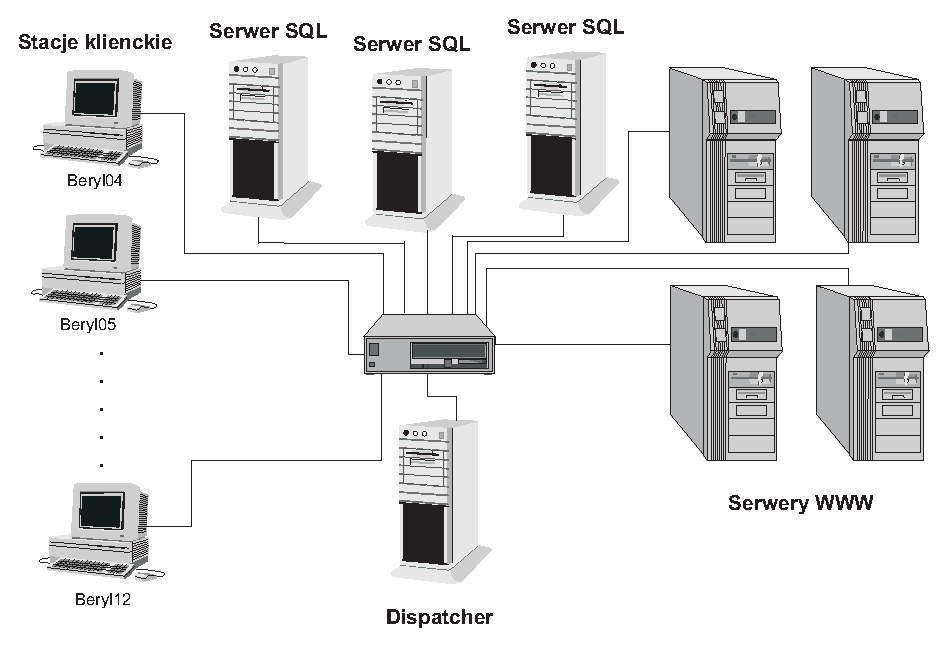
\includegraphics[width=14cm]{./rysunki/komputerki.eps}
\caption{Architektura segmentu sieci testowej.}
\label{architektura}
\end{figure}
Ka�dy komputer wyposa�ony by� w procesor Intel 
Celeron 300 MHz, 96 MB pami�ci SDRAM, dysk twardy o pojemno�ci 3 GB oraz kart� sieciow� 3COM EtherLink XL (10/100 Mbps). 
P�yta g��wna ka�dego komputera zbudowana by�a w oparciu o chipset Intel 430 LX. Komputery te posiada�y adresy IP z zakresu 
156.17.130.69 -- 156.17.130.79 i nazwy odpowiednio Beryl04 -- Beryl12. Na komputerach tych zainstalowane by�o oprogramowanie
Astra LoadRunner firmy Mercury Interactive. Komputery o identycznej architekturze stanowi�y serwery baz danych: beryl01 (IP = .66), beryl02 (IP = .67), beryl03 (IP = .68).
Zainstalowano na nich MS SQL server w wersji 7.0 (wersja 120 dniowa) wraz z baz� testow�.

Poza wy�ej wymienionymi komputerami PC pod��czony by�y badany klaster serwer�w WWW. Sprz�tow� platform� serwer�w by�y 
komputery IBM RS 6000 43P Model 260 pracuj�ce pod kontrol� systemu operacyjnego AIX 4.3.3. Ka�dy z tych komputer�w posiada� 
256 MB pami�ci RAM, dysk twardy UW SCSI o pojemno�ci 4.3 GB oraz zintegrowan� kart� sieciow� IBM 10/100 Mbps. ,,Sercem'' tej 
serii komputer�w RS 6000 jest procesor RISC PowerPC Power3 taktowany cz�stotliwo�ci� 200 Mhz. Trzy z wykorzystywanych maszyn 
posiada�y jeden taki procesor a dwa wyposa�one by�y w dwa procesory po��czone w architekturze SMP. Na ka�dym z badanych 
serwer�w zainstalowane by�o oprogramowanie serwera WWW Apache for AIX. Poszczeg�lne komputery RS 6000 posiada�y adresy IP z 
zakresu 156.17.130.45 -- 156.17.130.49 i nazwy odpowiednio akwamaryn (RS/6000 dwuprocesorowy), szafir (dwuprocesorowy), 
opal01 -- opal03 (jednoprocesorowe). Jedna maszyna dwuprocesorowa (szafir) pos�u�y�a do 
rozpropagowania obci��enia (dispatcher+CBR i WTE), druga pos�u�y�a do obs�ugi ��da� o statyczne
pliki HTML, za� pozosta�e maszyny obs�ugiwa�y dynamicznie generowane (poprzez skrypty PHP) strony,
w ten spos�b, �e ka�dy z opali pobiera� dane z bazy danych poszczeg�lnych beryli (opal01--beryl01,
 opal02--beryl02 i opal03--beryl03).

Wszystkie komputery by�y po��czone ze 100Mbps switchem OmniS/R-5 firmy Alcatel. R�wnie� wyj�cie na Swiat by�o realizowane z
t� szybko�ci�. 

Konstrukcja zarz�dzanego, wielokomputerowego systemu WWW by�a bardzo z�o�ona. Sk�ada�a si� z 
nast�puj�cych element�w:
\begin{enumerate}
\item Instalacja i konfiguracja switcha OmniSwitch/Router firmy Alcatel;
\item Instalacja i konfiguracja dispatchera z modu�em CBR. W sk�ad tej cz�ci wesz�y: 
\begin{itemize}
\item instalacja systemu AIX w wersji 4.3.3 oraz jego update do wersji 4.3.3.0.8 (niezb�dne pliki
zosta�y �ci�gni�te z odpowiedniej strony firmy IBM;
\item instalacja wirtualnej maszyny (VM) Javy w wersji 1.3.0;
\item instalacja oprogramowania IBM WebSphere Edge Server 1.0.3  wraz z 60--dniow� licencj�;
\item skonfigurowanie WTE jako \emph{reverse proxy } o adresie URL: www1.ists.pwr.wroc.pl, kt�ry
przekierowywa� adresy URL do serwer�w: opal01, opal02, opal03 i akwamaryn, w ten spos�b, aby
��dania o statyczne pliki HTML zosta�y skierowane do serwera akwamaryn, za� ��dania o dynamicznie
generowane strony z rozszerzeniami: .PHP, .PHP3 i PHP4 zosta�y rozpropagowane na pozosta�e
trzy maszyny;
\end{itemize}
\item Instalacja i konfiguracja oprogramowania dodatkowego na poszczeg�lne serwery WWW i 
dispatchera tzn. HTTP Server Apache w wersji 1.3.19, kompilator C i C++ w postaci gcc w wersji
2.95.3 oraz j�zyka skryptowego PHP w wersji 4.0.6;
\item Instalacja i konfiguracja Windows NT 4.0 Server wraz z Service Pack 6.0 na dwunastu
laboratoryjnych komputerach PC;
\item Instalacja i konfiguracja Microsoft SQL Serwera w wersji 7.0 na serwerach baz danych oraz
instalacja bazy testowej;
\item Instalacja oprogramowania do test�w na pozosta�ych komputerach; przygotowanie testu;
\item przygotowanie witryny WWW do test�w;
\end{enumerate}

\subsection{Algorytmy i metody}
Poni�ej znajduj� si� opisane trzy powsta�e modele. W ka�dym z nich program komputer (RS/6000) wraz z zainstalowanym programem 
IBM SecureWay Network Dispatcher stanowi uk�ad rozdysponuj�cy ��daniami. 

\subsubsection{Information less -- modu� dispatcher + Round Robin}

Sam Dispatcher nie ma mo�liwo�ci pracy w statycznym algorytmie Round Robin, jednak�e (jak napisano powy�ej, w charakterystyce 
oprogramowania) mo�na pos�ugiwa� si� modu�em Dispatcher z wy��czonym modu�em Zarz�dcy oraz z og�rnie nadanymi wagami. W tym
przypadku, pomimo niehomogenicznego �rodowiska nadano wszystkim elementom klastra WWW wagi r�wne jeden. W tej sytuacji komputer
z zainstalowanym dispatcherem r�wnomiernie (bez jakiejkolwiek analizy) propagowa� ��dania do poszczeg�lnych komputer�w.

W tym przypadku dost�p do bazy danych m�g� by� realizowany z dowolnego komputera (serwera WWW).

\subsubsection{Server info aware -- modu� dispatcher + Weighted Round Robin}

W por�wnaniu do poprzedniego przypadku w tym u�yto Dispatchera z uruchomionym modu�em zarz�dcy. Wtedy te� realizowany by�
algorytm Wa�ony Round--Robin. Wagi nadawane by�y dynamicznie tzn. w zale�no�ci od obci��enia poszczeg�lnych komputer�w -- 
serwer�w WWW. 

W tym jak i w powy�szym przypadku dost�p do bazy m�g� by� r�wnie� realizowany z dolwolnego z serwer�w WWW.

\subsubsection{Client info aware -- modu� CBR + WTE}

By� to najbardziej z�o�ony przypadek. Ka�dy pakiet by� analizowany pod wzgl�dem typu zawarto�ci oraz pod wzgl�dem jego 
obecno�ci w keszu komponentu WTE. CBR zosta� tak skonfigurowany aby rozpoznawa� URL z zawartym w nim wyrazem .php 
(identyfikuj�cym plik HTML z zawartym kodem PHP dost�pu do bazy). Pozwoli�o to na rozdzdzia� zapyta� na ��dania o pliki
statyczne (te by�y rozsy�ane go trzech jednoprocesorowych maszyn RS/6000), za� te ��dania o pliki, kt�rych cz�� by�a
generowana dynamicznie by�y przekazywane na dwuprocesorowy serwer, kt�ry komunikowa� sie (tylko on) z serwerem baz danych.
Taka konfiguracja pozwoli�a rozdysponowa� zar�wno obci��enie jak i typ po��cze�.

\subsection{Metodologia testowania}

Celem testowania powsta�ego systemu do zarz�dzania wielokomputerowym serwerem WWW
jest zbadanie wydolno�ci takiego systemu -- tzn. jego wydajno�ci w sytuacji
maksymalnego obci��enia, czyli tak�e mo�liwo�ci odpowiedzi na klienckie 
��danie w takiej sytuacji. Zamierzeniem testowania jest odpowied� na 
pytanie jak obci��enie jest r�wnowa�one pomi�dzy poszczeg�lnymi cz�ciami
sk�adowymi systemu, w zale�no�ci od algorytmu dysypacji obci��enia
(Round--Robin, Weighted Round--Robin oraz rozproszenie oparte na CBR), oraz
jaki dany algorytm ma wp�yw na LB.

Testowanie zaprojektowanego rozproszonego serwera WWW polega�o na pomiarze
wydajno�ci tak wej�ciowej jak i wyj�ciowej ca�ego systemu jak i poszczegolnych
jego sk�adowych (poszczeg�lnych serwer�w WWW, serwera baz danych i dispatchera).

Celem testowania by�o zbadanie maksymalnej wydajno�ci systemu. Wydajno�� systemu mo�na bada� na kilka sposob�w:
\begin{itemize}
\item ilo�� zapyta� w czasie,
\item ilo�� danych przes�anych w czasie.
\end{itemize}

Na wynik wp�yw ma informacja w jaki spos�b roz�o�one by�y zapytania oraz czy sesje ko�czy�y si� prawid�owo. Za�o�ono trzy 
mo�liwo�ci odpowiedzi systemu:
\begin{itemize}
\item w czasie do 3 s.,
\item w czasie 5 s.,
\item odpowiedz powy�ej 8 s.
\end{itemize}

Za sesj� prawid�owo zako�czon� uznno tak�, podczas kt�rej dwie kolejne odpowiedzi na pytania nie przekroczy�y 8 s.

Za�o�ono nast�puj�ce �cie�ki poruszania si� po serwisie \cite{savoia3}:
\begin{itemize}
\item \emph{Home ---> Exit} (Home -- strona domowa);
\item \emph{Home ---> First Level ---> Exit} (First Level -- np. informacja o produkcie);
\item \emph{Home ---> First Level ---> Object ---> Exit} (Object -- np. zakup).
\end{itemize}
Przy za�o�eniu, �e ruch na ,,typowej'' witrynie \cite{savoia1,savoia2,savoia3} wygl�da w nast�puj�cy spos�b:
\begin{itemize}
\item \emph{Home} -- 58 \%;
\item \emph{First Level} -- 31 \%;
\item \emph{Object} -- 11 \%;
\end{itemize}

Na bazie powy�szych danych nale�y zbudowa� skrypty generuj�ce zapytania.

\subsubsection{Analiza wynik�w}

Aby prawid�owo odpowiedzie� na pytanie zwi�zane z wydajno�ci� i dost�pno�ci� systemu nale�y poda�, 
przy jakiej ilo�ci u�ytkownik�w system jest w stanie prawid�owo odpowiada� czyli
przy \emph{x} u�ytkownik�w (otwartych sesji) system odpowiada (pomiary zostaj� wykonanywane w okre�lonych przedzia�ach 
czasowych):
\begin{itemize}
\item \% w czasie do 3 s.
\item \% w czasie do 5 s.
\item \% powy�ej 8 s.
\end{itemize}

Je�eli podczas sesji dwie nast�puj�ce po sobie odpowiedzi przekroczy�y 8s. -- oznacza to, �e ich sesje zosta�y zerwane.
System nie mo�e by� obci��ony w wi�kszym stopniu ni� aktualny aby wszystkie nap�ywaj�ce do niego sesje zosta�y 
prawid�owo obs�u�one.

Tak zaplanowane testy nale�y wykona� podczas pracy Dispatcher--a z r�nymi algorytmami: Round Robin, Multi Class Round Robin,
Weighted Round Robin. Wyniki powy�szych test�w pozwalaj� sprawdzi�, jak zachowuje si� system w przypadku chwilowego du�ego 
obci��enia. 

Kolejnym elementem test�w by�oby zasymulowanie normalnych warunk�w pracy systemu na granicy 80 \% wydajno�ci. Podczas takiej 
pracy nale�a�oby wygenerowa� obci��enie znacznie przewy�szaj�ce mo�liwo�ci systemu. Obci��enie to powinno trwa� 3s, 5s, wi�cej 
ni� 8s. Pozwoli to sprawdzi� jak system reaguje i jak szybko jest w stanie si� ustabilizowa� doprowadzaj�c do r�wnego 
roz�o�enia obci��enia na poszczeg�lne serwery. 
\section{Wyniki wst�pnych eksperyment�w}

Na skutek powa�nych problem�w, tak sprz�towych jak i programowych autor pracy nie zdo�a� 
zrealizowa� wszystich zaplanowanych zada�. Poni�ej wymieniono kolejne elementy budowy systemu do zarz�dzania wielokomputerowym
serwerem WWW oraz stopie� ich realizacji. 
\begin{enumerate}
\item przygotowano �rodowisko serwer�w front--endowych oraz dispatchera:
\begin{itemize}
\item uruchomiono oraz zainstalowano system operacyjny AIX 4.3.3 na komputerach IBM RS/6000, ktore mia�y stanowi� serwer
dispatchera, oraz cztery serwery WWW; na tych r�wnie� maszynach wykonano niezb�dny update do wersji 4.3.3.0.8;
\item zainstalowano menad�er pakiet�w RPM, kompilator gcc 2.95.3, Apache 1.3.19 oraz j�zyk skryptowy PHP 4.0.6 (za jego pomoc�
nale�a�o stworzy� interface pomi�dzy serwerem WWW a serwerem baz danych) -- jako modu� �adowalny do serwera Apache;
\item skonfigurowano ka�dy z serwer�w WWW wraz z modu�em �adowalnym PHP;
\item zainstalowano i skonfigurowano IBM WebSphere Edge Server jako \emph{reverse proxy} wraz z modu�em CBR odpowiedzialnym
za specyficzne, oparte na regu�ach przekierowywanie ��da�; podczas instalacji napotkano jednak�e na dwa powa�ne problemy, kt�re
uniemo�liwia�y instalacj�, a tym samym dzia�anie pakietu: modu� dispatcher nie uruchamia� si� zg�aszaj�c brak pliku licencji,
za� WTE nie uruchamia� si� z powodu niekompatybilno�ci z g��wn� bibliotek� systemow� (libc.a) (na obie sytuacje nie znaleziono
pomocy w �adnej posiadanej literaturze); skorzystano z \emph{supportu} firmy IBM; w pierwszym przypadku -- otrzymano poprawny
plik licencyjny, za� w drugim rozwi�zaniem okaza�o si� prze��czenie urz�dze� I/O w tryb asynchroniczny; po wykonaniu obu zada�
oraz skonfigurowaniu modu��w -- dispatcher + WTE dzia�a�o poprawnie;
\end{itemize}
\item przygotowano �rodowisko serwer�w back-endowych (baz danych):
\begin{itemize}
\item zainstalowano na trzech komputerach PC system operacyjny Windows NT 4.0 Server wraz z serwerem baz danych Microsoft
SQL Server 7.0 (wersja 120--dniowa), nast�pnie skonfigurowano te maszyny;
\item zainstalowano baz� testow� na serwerach;
\end{itemize}
\item system testowy Astra LoadRunner; niestety nie uda�o si� uzyska� tego oprogramowania testowego z powodu braku wersji 
testowej (komercyjna kosztuje oko�o 13000\$); uzyskano jednak�e program Astra LoadTest o zbli�onej funkcjonalno�ci (wersja 
testowa na dzisi�ciu wirtualnych u�ytkownik�w dzia�aj�ca bez ogranicze� 7 dni); zosta� zainstalowany i sprawdzony w kierunku
wymaga� tej pracy; wykonano za jego pomoc� wst�pny, przyk�adowy test, opis i wyniki znajduj� si� 
w Dodatku;
\end{enumerate}

Po poprawnym wykonaniu wy�ej wymienionych czynno�ci autor pracy stan�� przed problemem pobierania danych z serwer�w baz danych
przez serwery WWW. Pakiet RPM j�zyka PHP zawiera� binarny modu� �adowalny do Apache skompilowany bez wsparcia w komunikacji
z bazami danych (poza samym modu�em �adowalnym istniej� jeszcze modu�y odpowiadaj�ce komunikacji z poszczeg�lnymi serwerami
baz danych). W zwi�zku z tym, �e PHP jest j�zykiem, kt�ry jest dost�pny w �r�d�ach (na licencji GPL) pr�bowano poprzez 
kompilacj� i odpowiedni� konfiguracj� w��czy� go do Apache. MS SQL Server jest serwerem baz danych opartym na motorze firmy 
Sybase, dlatego aby nawi�za� komunikacj� z serwera WWW do serwera bazy danych MS SQL poprzez PHP nale�a�o przygotowa� 
(przekompilowa�) odpowiednie modu�y (klienty) PHP w formie modu��w �adowalnych. Niestety z powodu braku odpowiedniego API
nie uda�o si� tego zadania zrealizowa� (aby m�c stworzy� klienty PHP do baz danych -- nale�y kompilowa� PHP wraz z API
odpowiedniego serwera bazy danych).

Pr�bowano tak�e skorzysta� z odpowiednich sterownik�w ODBC firmy OpenLink\footnote{http://www.openlinksw.com}. Poza 
ograniczeniami w korzystaniu z tego oprogramowania (mo�liwo�� pracy tylko dw�ch jednoczesnych u�ytkownik�w podczas sesji) nie
uda�o si� przekompilowa� PHP (wyst�powa�y b��dy podczas kompilacji). Podczas poszukiwania rozwi�zania w Internecie, skorzystano
r�wnie� z mo�liwo�ci Usenetu (listy dyskusyjne).

Powy�szego problemu nie uda�o si� r�wnie� rozwi�za� analizuj�c zmian� j�zyka oprogramowania: PERL (kolejny znakomity j�zyk 
skryptowy umo�liwiaj�cy generowanie stron dynamicznych) -- ma zbli�one wymagania je�li chodzi o klient�w baz danych, ASP (nie 
istnieje na maszyny Unixowe), C, C++ lub Java (du�e k�opoty implementacyjne, spora pracoch�onno��).

W zwi�zku z brakiem mo�liwo�ci scalenia sewer�w WWW z serwerami baz danych nie uda�o si� przetestowa� w pe�ni dzia�aj�cego
systemu do zarz�dzania wielokomputerowym serwisem WWW.

\chapter*{Dodatek}

\section*{Test}

W związku z awarią sieci teleinformatycznej w Instytucie Sterowania i Techniki Systemów poniższy 
próbny test przeprowadzono 
na skonstruowanym wielokomputerowym systemie WWW za pomocą tylko jednej maszyny komunikującej się z 
systemem za pomocą 10MB huba (firmy IBM). 

Na kolejnych stronach znajdują się wynikowe zestawienia i wykresy próbnego testu wykonanego za 
pomocą oprogramowania Astra LoadTest. Test został wykonany z dziesięcioma wirtualnymi 
użytkownikami\footnote{\emph{Vusers}} (uruchamianymi w kolejności co 15 sek.) poruszającymi się po 
znajdującej się na systemie WWW dokumentacji do serwera Apache (razem dziesięć dowolnie wybranych 
stron). Trwał on 6 min. i 19 sek. Jak widać na rys. \ref{zebrane} łącznie przesłano: $19 915 485$ 
bajtów ze średnią przepustowością na poziomie 52 kb/sek; łącznie $1 925$ trafień (średnio pięć na 
sekundę). Również na rys. \ref{zebrane} znajduje się tabela transakcji wraz ze średnim, minimalnym 
i maksymalnym czasem jej realizacji.

Na rys. \ref{wydajnosc} widać wykres przepustowości serwisu WWW w bajtach na sekundę. Poniżej wykresu 
znajduje się jego charakterystyka wraz z odchyleniem standardowym i medianą.

Kolejny rysunek (rys. \ref{zadania_sekunde}) przedstawia wykres ilości trafień na sekundę 
(charakterystyka wykresu poniżej).

Następny wykres (rys. \ref{pobierana_strona}) przedstawia zależność ilości transakcji od pobranej strony.

Na wykresie (rys. \ref{srednia_odpowiedz}) widać średni czas realizacji transakcji (każdej strony). 
Rys. \ref{zestawienie_odpowiedzi} zawiera zestawienie średnich, najkrótszych i najdłuższych czasów 
realizacji transakcji, a rys. \ref{procentowo} procentowy rozkład ilości transakcji w czasie.

Wykres na rysunku \ref{stron_sekunda} obrazuje ilość pobranych stron na sekundę.

\begin{figure}[h]
\centering
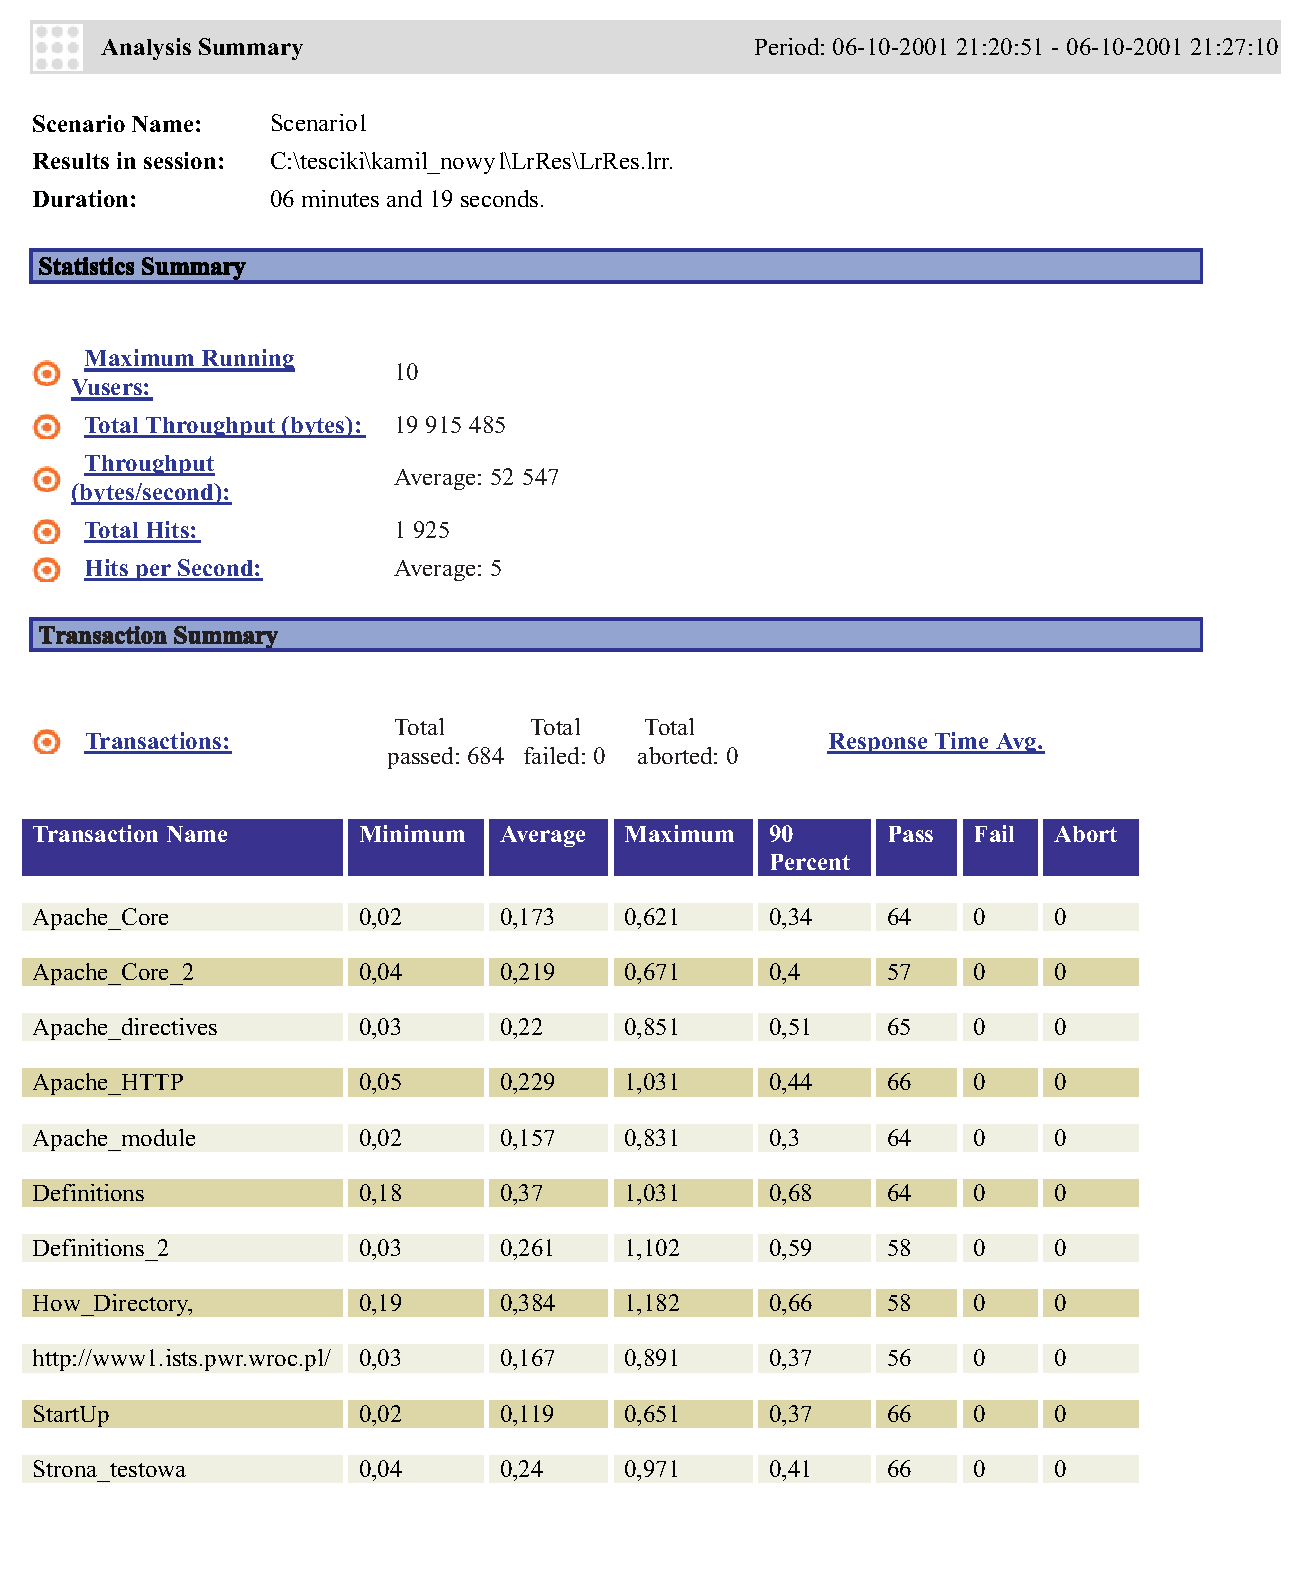
\includegraphics[width=\textwidth]{./rysunki/summary-test.eps}
\caption{Zebrane informacje o przebiegu testu}
\label{zebrane}
\end{figure}
\begin{figure}[h]
\centering

\includegraphics[width=4.5in]{./rysunki/raport1calybokiem.eps}
\caption{Wydajność wielokomputerowego systemu WWW}
\label{wydajnosc}
\end{figure}
\begin{figure}[h]
\centering

\includegraphics[width=4.5in]{./rysunki/raport2calybokiem.eps}
\caption{Ilość realizacji żądań na sekundę}
\label{zadania_sekunde}
\end{figure}
\begin{figure}[h]
\centering

\includegraphics[width=4.5in]{./rysunki/rapor3calybokiem.eps}
\caption{Ilość transakcji w zależności od pobieranej strony}
\label{pobierana_strona}
\end{figure}
\begin{figure}[h]
\centering
\includegraphics[width=\textwidth]{./rysunki/raport4calybokiem.eps}
\caption{Średni czas odpowiedzi}
\label{srednia_odpowiedz}
\end{figure}
\begin{figure}[h]
\centering
\includegraphics[width=4.5in]{./rysunki/raport7calybokiem.eps}
\caption{Zestawienie odpowiedzi w zależności od pobieranej strony}
\label{zestawienie_odpowiedzi}
\end{figure}
\begin{figure}[h]
\centering
\includegraphics[width=\textwidth]{./rysunki/raport9calybokiem.eps}
\caption{Czas odpowiedzi transakcji -- udział procentowy}
\label{procentowo}
\end{figure}
\begin{figure}[h]
\centering
\includegraphics[width=\textwidth]{./rysunki/raport10calybokiem.eps}
\caption{Czas odpowiedzi transakcji -- rozkład}
\label{odpowiedz_transakcji_rozklad}
\end{figure}
\begin{figure}[h]
\centering

\includegraphics[width=4.5in]{./rysunki/raport11calybokiem.eps}
\caption{Liczba stron na sekundę}
\label{stron_sekunda}
\end{figure}




\addcontentsline{toc}{chapter}{Literatura}
\bibliography{literatura}

\addcontentsline{toc}{chapter}{Spis Rysunków}
{\footnotesize\listoffigures}


\end{document}
